% Options for packages loaded elsewhere
\PassOptionsToPackage{unicode}{hyperref}
\PassOptionsToPackage{hyphens}{url}
\PassOptionsToPackage{dvipsnames,svgnames,x11names}{xcolor}
%
\documentclass[
  a4paper,
]{ltjsbook}

\usepackage{amsmath,amssymb}
\usepackage{iftex}
\ifPDFTeX
  \usepackage[T1]{fontenc}
  \usepackage[utf8]{inputenc}
  \usepackage{textcomp} % provide euro and other symbols
\else % if luatex or xetex
  \usepackage{unicode-math}
  \defaultfontfeatures{Scale=MatchLowercase}
  \defaultfontfeatures[\rmfamily]{Ligatures=TeX,Scale=1}
\fi
\usepackage{lmodern}
\ifPDFTeX\else  
    % xetex/luatex font selection
\fi
% Use upquote if available, for straight quotes in verbatim environments
\IfFileExists{upquote.sty}{\usepackage{upquote}}{}
\IfFileExists{microtype.sty}{% use microtype if available
  \usepackage[]{microtype}
  \UseMicrotypeSet[protrusion]{basicmath} % disable protrusion for tt fonts
}{}
\makeatletter
\@ifundefined{KOMAClassName}{% if non-KOMA class
  \IfFileExists{parskip.sty}{%
    \usepackage{parskip}
  }{% else
    \setlength{\parindent}{0pt}
    \setlength{\parskip}{6pt plus 2pt minus 1pt}}
}{% if KOMA class
  \KOMAoptions{parskip=half}}
\makeatother
\usepackage{xcolor}
\usepackage[top=30mm,left=20mm,heightrounded]{geometry}
\setlength{\emergencystretch}{3em} % prevent overfull lines
\setcounter{secnumdepth}{5}
% Make \paragraph and \subparagraph free-standing
\ifx\paragraph\undefined\else
  \let\oldparagraph\paragraph
  \renewcommand{\paragraph}[1]{\oldparagraph{#1}\mbox{}}
\fi
\ifx\subparagraph\undefined\else
  \let\oldsubparagraph\subparagraph
  \renewcommand{\subparagraph}[1]{\oldsubparagraph{#1}\mbox{}}
\fi

\usepackage{color}
\usepackage{fancyvrb}
\newcommand{\VerbBar}{|}
\newcommand{\VERB}{\Verb[commandchars=\\\{\}]}
\DefineVerbatimEnvironment{Highlighting}{Verbatim}{commandchars=\\\{\}}
% Add ',fontsize=\small' for more characters per line
\usepackage{framed}
\definecolor{shadecolor}{RGB}{241,243,245}
\newenvironment{Shaded}{\begin{snugshade}}{\end{snugshade}}
\newcommand{\AlertTok}[1]{\textcolor[rgb]{0.68,0.00,0.00}{#1}}
\newcommand{\AnnotationTok}[1]{\textcolor[rgb]{0.37,0.37,0.37}{#1}}
\newcommand{\AttributeTok}[1]{\textcolor[rgb]{0.40,0.45,0.13}{#1}}
\newcommand{\BaseNTok}[1]{\textcolor[rgb]{0.68,0.00,0.00}{#1}}
\newcommand{\BuiltInTok}[1]{\textcolor[rgb]{0.00,0.23,0.31}{#1}}
\newcommand{\CharTok}[1]{\textcolor[rgb]{0.13,0.47,0.30}{#1}}
\newcommand{\CommentTok}[1]{\textcolor[rgb]{0.37,0.37,0.37}{#1}}
\newcommand{\CommentVarTok}[1]{\textcolor[rgb]{0.37,0.37,0.37}{\textit{#1}}}
\newcommand{\ConstantTok}[1]{\textcolor[rgb]{0.56,0.35,0.01}{#1}}
\newcommand{\ControlFlowTok}[1]{\textcolor[rgb]{0.00,0.23,0.31}{#1}}
\newcommand{\DataTypeTok}[1]{\textcolor[rgb]{0.68,0.00,0.00}{#1}}
\newcommand{\DecValTok}[1]{\textcolor[rgb]{0.68,0.00,0.00}{#1}}
\newcommand{\DocumentationTok}[1]{\textcolor[rgb]{0.37,0.37,0.37}{\textit{#1}}}
\newcommand{\ErrorTok}[1]{\textcolor[rgb]{0.68,0.00,0.00}{#1}}
\newcommand{\ExtensionTok}[1]{\textcolor[rgb]{0.00,0.23,0.31}{#1}}
\newcommand{\FloatTok}[1]{\textcolor[rgb]{0.68,0.00,0.00}{#1}}
\newcommand{\FunctionTok}[1]{\textcolor[rgb]{0.28,0.35,0.67}{#1}}
\newcommand{\ImportTok}[1]{\textcolor[rgb]{0.00,0.46,0.62}{#1}}
\newcommand{\InformationTok}[1]{\textcolor[rgb]{0.37,0.37,0.37}{#1}}
\newcommand{\KeywordTok}[1]{\textcolor[rgb]{0.00,0.23,0.31}{#1}}
\newcommand{\NormalTok}[1]{\textcolor[rgb]{0.00,0.23,0.31}{#1}}
\newcommand{\OperatorTok}[1]{\textcolor[rgb]{0.37,0.37,0.37}{#1}}
\newcommand{\OtherTok}[1]{\textcolor[rgb]{0.00,0.23,0.31}{#1}}
\newcommand{\PreprocessorTok}[1]{\textcolor[rgb]{0.68,0.00,0.00}{#1}}
\newcommand{\RegionMarkerTok}[1]{\textcolor[rgb]{0.00,0.23,0.31}{#1}}
\newcommand{\SpecialCharTok}[1]{\textcolor[rgb]{0.37,0.37,0.37}{#1}}
\newcommand{\SpecialStringTok}[1]{\textcolor[rgb]{0.13,0.47,0.30}{#1}}
\newcommand{\StringTok}[1]{\textcolor[rgb]{0.13,0.47,0.30}{#1}}
\newcommand{\VariableTok}[1]{\textcolor[rgb]{0.07,0.07,0.07}{#1}}
\newcommand{\VerbatimStringTok}[1]{\textcolor[rgb]{0.13,0.47,0.30}{#1}}
\newcommand{\WarningTok}[1]{\textcolor[rgb]{0.37,0.37,0.37}{\textit{#1}}}

\providecommand{\tightlist}{%
  \setlength{\itemsep}{0pt}\setlength{\parskip}{0pt}}\usepackage{longtable,booktabs,array}
\usepackage{calc} % for calculating minipage widths
% Correct order of tables after \paragraph or \subparagraph
\usepackage{etoolbox}
\makeatletter
\patchcmd\longtable{\par}{\if@noskipsec\mbox{}\fi\par}{}{}
\makeatother
% Allow footnotes in longtable head/foot
\IfFileExists{footnotehyper.sty}{\usepackage{footnotehyper}}{\usepackage{footnote}}
\makesavenoteenv{longtable}
\usepackage{graphicx}
\makeatletter
\def\maxwidth{\ifdim\Gin@nat@width>\linewidth\linewidth\else\Gin@nat@width\fi}
\def\maxheight{\ifdim\Gin@nat@height>\textheight\textheight\else\Gin@nat@height\fi}
\makeatother
% Scale images if necessary, so that they will not overflow the page
% margins by default, and it is still possible to overwrite the defaults
% using explicit options in \includegraphics[width, height, ...]{}
\setkeys{Gin}{width=\maxwidth,height=\maxheight,keepaspectratio}
% Set default figure placement to htbp
\makeatletter
\def\fps@figure{htbp}
\makeatother

\makeatletter
\@ifpackageloaded{bookmark}{}{\usepackage{bookmark}}
\makeatother
\makeatletter
\@ifpackageloaded{caption}{}{\usepackage{caption}}
\AtBeginDocument{%
\ifdefined\contentsname
  \renewcommand*\contentsname{Table of contents}
\else
  \newcommand\contentsname{Table of contents}
\fi
\ifdefined\listfigurename
  \renewcommand*\listfigurename{List of Figures}
\else
  \newcommand\listfigurename{List of Figures}
\fi
\ifdefined\listtablename
  \renewcommand*\listtablename{List of Tables}
\else
  \newcommand\listtablename{List of Tables}
\fi
\ifdefined\figurename
  \renewcommand*\figurename{Figure}
\else
  \newcommand\figurename{Figure}
\fi
\ifdefined\tablename
  \renewcommand*\tablename{Table}
\else
  \newcommand\tablename{Table}
\fi
}
\@ifpackageloaded{float}{}{\usepackage{float}}
\floatstyle{ruled}
\@ifundefined{c@chapter}{\newfloat{codelisting}{h}{lop}}{\newfloat{codelisting}{h}{lop}[chapter]}
\floatname{codelisting}{Listing}
\newcommand*\listoflistings{\listof{codelisting}{List of Listings}}
\makeatother
\makeatletter
\makeatother
\makeatletter
\@ifpackageloaded{caption}{}{\usepackage{caption}}
\@ifpackageloaded{subcaption}{}{\usepackage{subcaption}}
\makeatother
\ifLuaTeX
  \usepackage{selnolig}  % disable illegal ligatures
\fi
\usepackage[style=../../biblatex-jpa/biblatex/jpa,]{biblatex}
\addbibresource{../../myBiber.bib}
\usepackage{bookmark}

\IfFileExists{xurl.sty}{\usepackage{xurl}}{} % add URL line breaks if available
\urlstyle{same} % disable monospaced font for URLs
\hypersetup{
  pdftitle={心理学統計実習},
  pdfauthor={Koji Kosugi},
  colorlinks=true,
  linkcolor={blue},
  filecolor={Maroon},
  citecolor={Blue},
  urlcolor={Blue},
  pdfcreator={LaTeX via pandoc}}

\title{心理学統計実習}
\usepackage{etoolbox}
\makeatletter
\providecommand{\subtitle}[1]{% add subtitle to \maketitle
  \apptocmd{\@title}{\par {\large #1 \par}}{}{}
}
\makeatother
\subtitle{Exercises in Psychological Statistics with R/RStudio}
\author{Koji Kosugi}
\date{}

\begin{document}
\maketitle

\renewcommand*\contentsname{Table of contents}
{
\hypersetup{linkcolor=}
\setcounter{tocdepth}{2}
\tableofcontents
}
\bookmarksetup{startatroot}

\chapter*{はじめに}\label{ux306fux3058ux3081ux306b}
\addcontentsline{toc}{chapter}{はじめに}

\markboth{はじめに}{はじめに}

この資料は,授業「心理学統計演習」についてのものです。
演習という授業名にあるように,理論的な解説で「理解して進む」ことよりも,「手を動かして理解する」ことを目的にしています。

この資料を活用する人は,理論的な(いわゆる座学の)心理学統計を履修済みであることを前提にしています。また,資料集という位置付けですので,行間の説明が省略されていることが多くあります。その点は講義時間中の講話で補完していくつもりですので,不明な点があれば授業時間中に質問してください。

\section*{ライセンス等}\label{ux30e9ux30a4ux30bbux30f3ux30b9ux7b49}
\addcontentsline{toc}{section}{ライセンス等}

\markright{ライセンス等}

この資料はCreative Commons BY-SA(CC BY-SA)ライセンスVersion
4.0に基づいて提供されています。
著者に適切なクレジットを与える限り,この本を再利用,再編集,保持,改訂,再頒布(商用利用を含む)をすることができます。
もし再編集したり,このオープンなテキストを変更したい場合,すべてのバージョンにわたってこれと同じライセンス,CC
BY-SA を適用しなければなりません。

This article is published under a Creative Commons BY-SA license (CC
BY-SA) version 4.0. This means that this book can be reused, remixed,
retained, revised and redistributed (including commercially) as long as
appropriate credit is given to the authors. If you remix, or modify the
original version of this open textbook, you must redistribute all
versions of this open textbook under the same license - CC BY-SA.

\bookmarksetup{startatroot}

\chapter{はじめようR/RStudio}\label{ux306fux3058ux3081ux3088ux3046rrstudio}

「R」。この一文字で表現されるがゆえに,検索しにくいことこの上ないそれは,統計に特化したプログラミング言語であり,心理学はもちろん統計に関する学問領域で多岐にわたって利用されているものである。フリーソフトウェア,すなわち自由で開かれているソフトウェアであるから,ソースコードに至るまで公開されており,誰でも無償で利用できる。無償すなわち無料ではない。補償がないので無償なのだが,逆に金銭で計算をはじめ科学的真実性が保証されるわけではない,という至極まともな考え方は理解できるだろう。科学はもちろん,ソフトウェアも人類の共有財産として,オープンに育んでいこう。

Rはコミュニティ活動も盛んで,Tokyo.Rを中心に日本の各地でRユーザからなる自主的な勉強会が開催されている\footnote{2024年1月現在で,TokyoだけでなくFukuoka,Sapporo,Yamaguchi,Irumaなどで地方コミュニティがあり,参加者みんなで楽しまれている。}。またR自体がインターネットを通じて公開されているように,導入から応用までさまざまな資料がオンラインで活用できる。以下では導入から解説していくが,頻繁にアップデートされるものでもあるので,必要に応じて検索し,なるべく時系列的に近い情報を吟味して活用することを薦める。

\section{環境の準備}\label{ux74b0ux5883ux306eux6e96ux5099}

\subsection{Rのインストール}\label{rux306eux30a4ux30f3ux30b9ux30c8ux30fcux30eb}

Rのインストールに関して,初心者でも利用可能な資料がオンラインで公開されている。

RはThe \href{https://cran.r-project.org/}{Comprehensive R Archive
Network},通称CRAN\footnote{CRANは「しーらん」,あるいは「くらん」と発音される。筆者はしーらん派。}というネットワークで公開されている。CRANのトップページにはダウンロードリンクが用意されており,自分のプラットフォームにあった最新版をダウンロードしよう\footnote{この授業のために自身のPCにRをインストールしたとして,次に使うときに半年以上間隔が空いたのなら,改めて最新版をチェックし,バージョンが上がっていたら旧版をアンインストールして最新版をインストールするところから始めた方が良い。Rで利用するパッケージなどが新しい版にしか対応していないことなどもある。Rと畳は新しい方が良い。}。

\subsection{RStudioのインストール}\label{rstudioux306eux30a4ux30f3ux30b9ux30c8ux30fcux30eb}

Rのインストールが終われば,次はRStudioをインストールしよう。
RStudioは総合開発環境(IDE)と呼ばれるものである。Rは単体で,統計の分析や関数の描画など,専門的な利用に耐えうる分析機能を有している。その本質はもちろん計算機能であって,計算を実行する命令文(スクリプト)を与えれば,必要な返答をあたえてくれる。このように分析の本質が計算機能であったとしても,実際の分析活動に際しては,スクリプトの下書きと清書,入出力データや描画ファイルの生成・管理,パッケージ(後述)の管理など,分析にまつわるさまざまな周辺活動が含まれる。喩えるなら料理の本質が包丁・まな板・コンロによる加工であったとしても,実際の調理に際しては,広い調理スペースや使いやすいシンク,ボウルやタッパーなどの補助的な調理器具があった方がスムーズにことが進む。
いわば,R単体で分析をするのは飯盒炊爨のような必要最低限かつワイルドな調理法であり,RStudioは総合的な調理環境を提供してくれるものなのである。

繰り返しになるが,本質的にはR単体で作業が可能である。なるべく単純な環境を維持したいというのであればR単体での利用を否定するものではないが,RStudioはエディタや文書作成ソフトとしても有用であるので,本授業ではRStudioを使うことを前提とする\footnote{VSCodeのようなエディタから使うことも可能であるし,Jupyter
  Notebookの計算エンジンをRにすることも可能。最近では分析ソフトウェアを個々人で準備せず,環境として提供することも一般的になってきており,例えば\href{https://colab.research.google.com/}{Google
  Colaboratory}のエンジンをRにすることもできるようになっている。ローカルPCに自前の環境を作るということが,時代遅れになる日も近いかもしれない。}。

\subsection{環境の準備に関する導入サイト}\label{ux74b0ux5883ux306eux6e96ux5099ux306bux95a2ux3059ux308bux5c0eux5165ux30b5ux30a4ux30c8}

以下に執筆時点(2024年1月)で参照可能な,導入に関するWeb教材を挙げておく。自分に合ったものを適宜参照し,RとRStudioを自身のPC環境に導入してほしい。もちろん自身で「R
RStudio
インストール」などとして検索しても良いし,chatGPTに相談しても良い。

\subsubsection{For Windows}\label{for-windows}

\begin{itemize}
\tightlist
\item
  東京大学・大学院農学生命科学研究科アグリバイオインフォマティクス教育研究プログラムによる\href{https://www.iu.a.u-tokyo.ac.jp/textbook/R/R1.010_win.pdf}{PDF資料}
\item
  \href{https://syunsuke.github.io/r_install_guide_for_beginners/}{初心者向けRのインストールガイド}
\item
  関西学院大学商学部土方ゼミ\href{http://soc-research.org/ja/r_install_windows/}{資料}
\item
  多摩大学情報社会研究所・応用統計学室\href{多摩大学情報社会研究所・応用統計学室}{資料}
\item
  奥村
  晴彦先生の\href{https://okumuralab.org/~okumura/stat/R-win.html}{ページ}
\end{itemize}

\subsubsection{For Macintosh}\label{for-macintosh}

\begin{itemize}
\tightlist
\item
  東京大学・大学院農学生命科学研究科アグリバイオインフォマティクス教育研究プログラムによる\href{https://www.iu.a.u-tokyo.ac.jp/textbook/R/R1.010_mac.pdf}{PDF資料}
\item
  noteの\href{https://note.com/toshi_matsuura/n/n127cf28362e5}{記事}
\item
  いちばんやさしい,医療統計\href{https://best-biostatistics.com/r/rstudio_start.html\#i-3}{記事}
\end{itemize}

なお,Macの場合はHomebrewなどのパッケージ管理ソフトを使って導入することもできる(し,そのほうがいい)。その場合は以下の資料を参照。

\begin{itemize}
\tightlist
\item
  群馬大学大学院医学系研究科機能形態学の\href{https://anatomy.med.gunma-u.ac.jp/protocols/?p=979}{記事}
\item
  コアラさばお氏のnote\href{https://note.com/mackerelman/n/nfbf8054e90d5}{記事}
\item
  Ryu
  Takahashi氏のQiita\href{https://qiita.com/ryu-takahashi2718/items/1118cad7a4ef4900da96}{記事}
\item
  Yuhki
  Yano氏のQiita\href{https://qiita.com/y-vectorfield/items/dd1a8e2715cace9981ec}{記事}
\end{itemize}

\section{RStudioの基礎(4つのペイン)}\label{rstudioux306eux57faux790euxff14ux3064ux306eux30daux30a4ux30f3}

ここまでで,RおよびRStudioを利用する準備が整っているものとする。

さて,RStudioを起動すると大きくわけて4つの領域に分かれた画面が出てくる。この領域のことを\textbf{ペイン}と呼ぶ。図中の「領域1」がないように見えるときもあるが,下のペインが最大化され折りたたまれているだけなので,ペイン上部のサイズ変更ボタンを操作することで出てくるだろう。

\begin{figure}[H]

{\centering 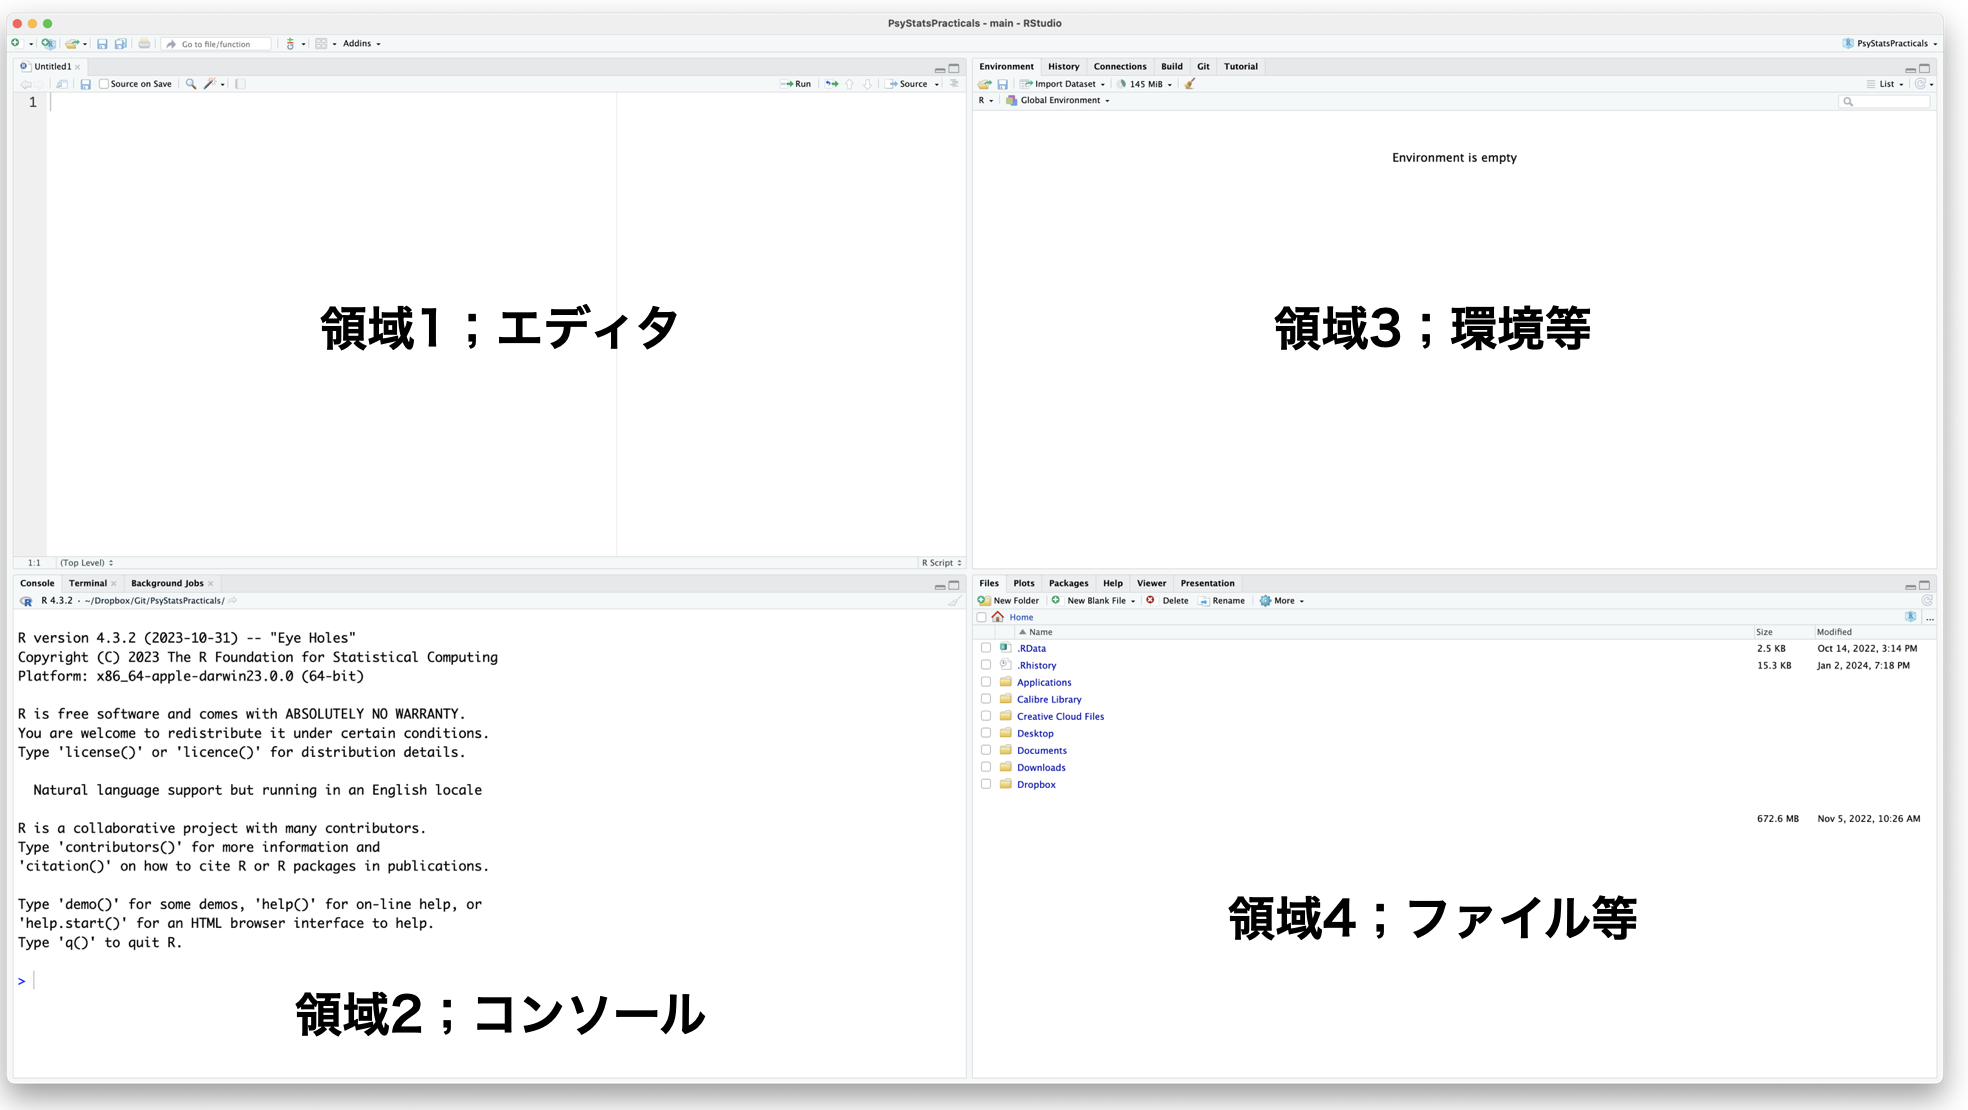
\includegraphics{../common/images/01_RStudioStart.png}

}

\caption{RStudioの初期画面}

\end{figure}%

このペインのレイアウトは,メニューのTools \textgreater{} Global
Options\ldots{} \textgreater{} Pane
Layoutから変更することもできる。基本的に4分割であることに変わりはないが,自分が利用しやすい位置にレイアウトを変更するとよい。

\begin{figure}[H]

{\centering 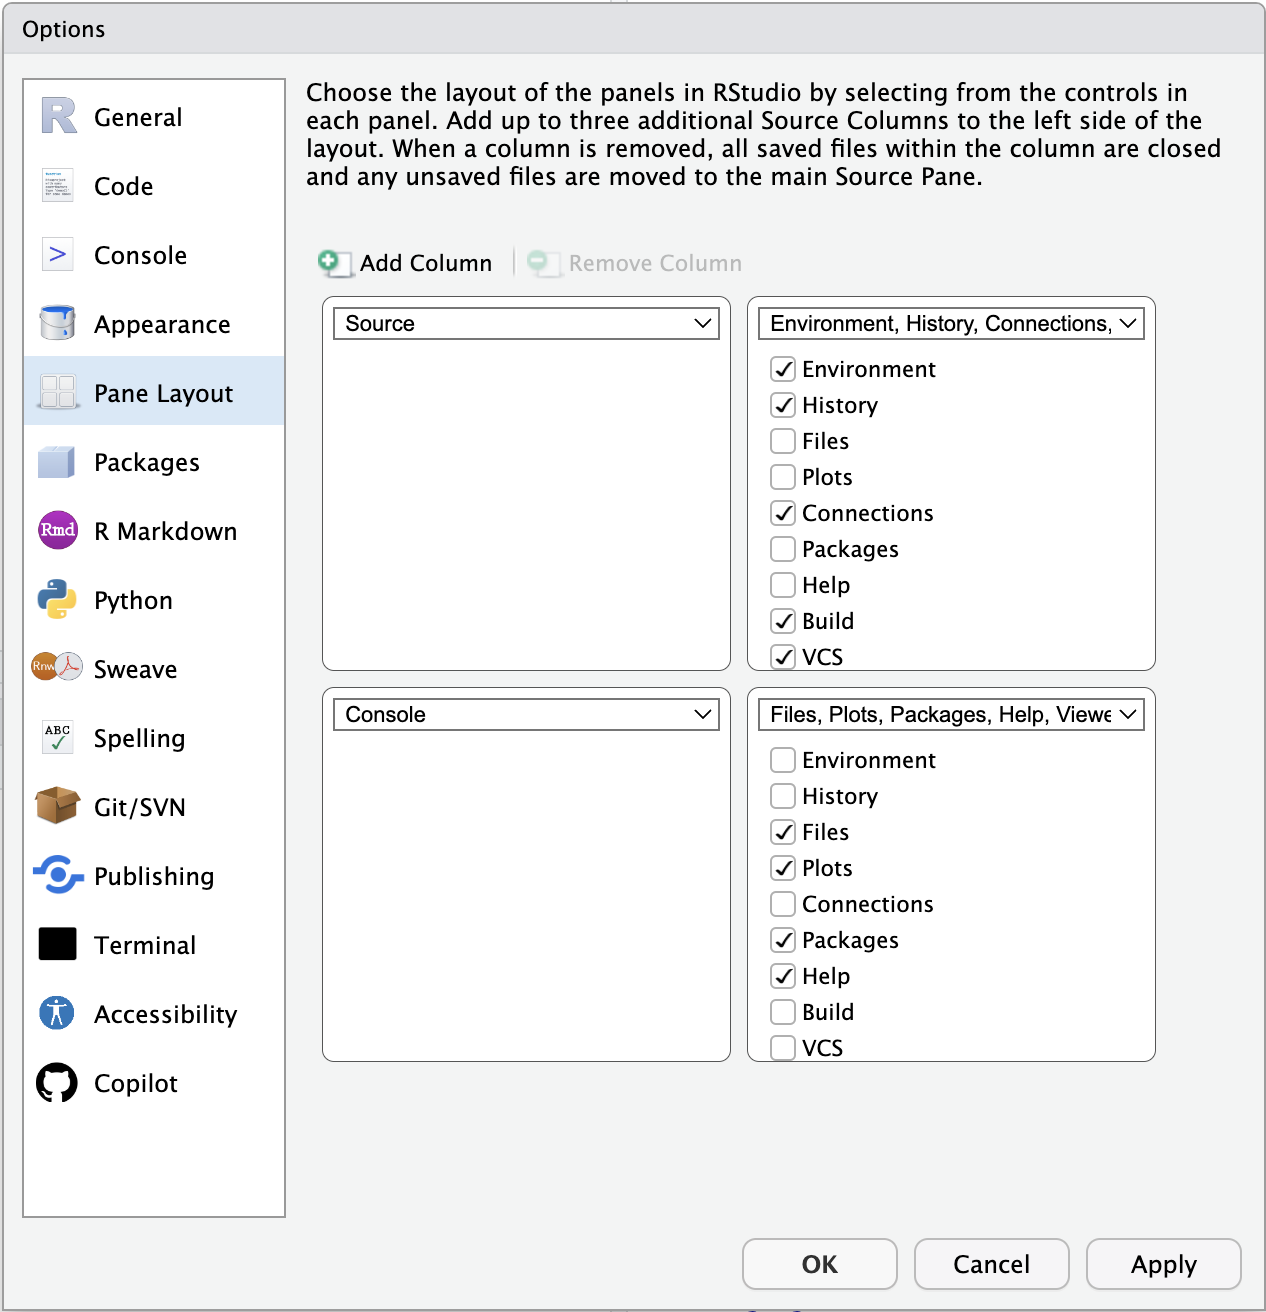
\includegraphics{../common/images/01_PaneLayout.png}

}

\caption{レイアウト変更画面。このほかにも背景色などを変えることもできる}

\end{figure}%

以下,各ペイン(領域)が何をするところかを簡単に解説する。

\subsection{領域1;エディタ・ペイン}\label{ux9818ux57df1ux30a8ux30c7ux30a3ux30bfux30daux30a4ux30f3}

エディタ領域。Rのスクリプトはもちろん,レポートの文章など,基本的に入力するときはこのペインに書く。ここで作業するファイルの種類は,File
\textgreater{} New
Fileから見ると明らかなように,R言語だけでなくC言語,Python言語などのスクリプトや,Rmd,md,Qmd,HTMLなどのマークアップ言語,StanやSQLなど特殊な言語などにも対応している。ペインの右下に現在開かれているファイルの種類が表示されているのを確認しておこう。

R言語でスクリプトを書く例で解説しよう。Rは命令を逐次実行していくインタプリタ形式であり,ここに記述されたRコードを,右上のRunボタンでコンソールに送って計算を実行するように使う。一回の命令をコマンド,コマンドが積み重ねられた全体をスクリプト,あるいはプログラムと呼ぶ。複数のコマンドを実行したい場合は,エディタ領域で複数行選択してRunボタンを,スクリプトファイル全体を実行したいときはRunボタンのとなりにあるSourceを押す。CTRL+Enter(Macの場合はコマンド+Enter)でRunボタンのショートカットになる。

\subsection{領域2;コンソール・ペイン}\label{ux9818ux57df2ux30b3ux30f3ux30bdux30fcux30ebux30daux30a4ux30f3}

R単体で利用する場合は,ここのペインだけを利用するようなものである。すなわち,ここに示されているのがR本体というか,Rの計算機能そのものである。ここに「>」の記号が表示されているところをプロンプトといい,プロンプトが表示されているときはRが入力待ちの状態である。

Rは逐次的に計算を行うので,プロンプトのある状態でコマンドを入力すると計算結果が返される。
ここに直接コマンドを書いて行っても良いが,書き間違えたりすることもあるし,コマンドが複数行に渡ることが一般的になってくるので,エディタ領域に清書するつもりで記述していったほうがよい。ごくたまに,一時的に確認したいことがある時だけ,直接コンソールを触るようにすると良い。

なお,コンソールを綺麗にしたいときは右上の箒ボタンをおすとよい。

\subsection{領域3;環境ペイン}\label{ux9818ux57df3ux74b0ux5883ux30daux30a4ux30f3}

基本的にこのペインと次の領域4のペインは複数のタブが含まれる。Pane
Layoutでどちらにどのタブを含めるかを自分好みにカスタマイズすることもできる。ここでは代表的な2つのタブについてのみ言及する。

\textbf{Environment}タブは,Rの実行メモリ内に保管されている変数や関数などが表示されている。「変数や関数など」をまとめて\textbf{オブジェクト}というが,ここで内容や構造をGUIで確認することができる。

\textbf{History}タブは履歴である。これまでコンソールに送られてきたコマンドが順に記録されている。Historyタブからエディタ,コンソールにコマンドを送ることも可能であり,「さっきの命令をもう一度実行したい」といったときに参照すると良い。

\subsection{領域4;ファイルペイン}\label{ux9818ux57df4ux30d5ux30a1ux30a4ux30ebux30daux30a4ux30f3}

ここでも代表的なタブについてのみ解説する。

\textbf{Files}タブはMacでいうFinder,Windowsでいうエクスプローラーのような,ファイル操作画面である。フォルダの作成,ファイルの削除,リネーム,コピーなどの操作が可能である。

\textbf{Plot}タブはRコマンドで描画命令が出された時の結果がここに表示される。RStudioの利点の一つは,このPlotから図をファイルにExportすることが可能であり,その際にファイルサイズやファイル形式を指定できるところにある。

\textbf{Packages}タブは読み込まれているパッケージ,(読み込まれていないが)保管しているパッケージのリストが表示されている。新しくパッケージを導入するときも,ここのinstallボタンから可能であり,保管しているパッケージのアップデートもボタンひとつで可能である。なお,パッケージについては後ほど言及する。

\textbf{Help}タブはRコマンドでヘルプを表示する命令(\texttt{help}関数)が実行された時の結果が表示される領域である。ヘルプを使うことで関数の引数,戻り値,使用例などを参照できる。

\subsection{そのほかのタブ}\label{ux305dux306eux307bux304bux306eux30bfux30d6}

そのほか,表示の有無もオプションになっているようないくつかのタブについて,簡単に解説しておく。

\textbf{Connections}タブはRを外部データベースなどに繋げるときに参照する。大規模データをローカルにすべて取り込むことなく,SQLで必要なテーブルだけ取り出すといった操作をする際は必要になってくるだろう。

\textbf{Git}タブはR,とくにRプロジェクト(後述)のバージョンを管理するときに利用する。Gitとは複数のプログラマによって同時並行的にプログラムを作っていく時の管理システムである。時系列的な差分の記録を得意とするシステムなので,レポートの作成時などに応用すればラボノートの記録としても利用できる。

\textbf{Build}タブはRパッケージやWebサイトを構築するときに利用する。なおこの資料もRStudioを利用して作られており,資料を生成(原稿からHTMLやPDFにする)ときにはこのタブを利用している。

\textbf{Tutorial}タブはチュートリアルツアーを楽しむ時のタブである。

\textbf{Viewer}タブはRStudioで作られたHTMLやPDFなどを見るためのタブである。

\textbf{Presentation}タブはRStudioで作られたプレゼンテーションを見るためのタブである。

\textbf{Terminal}タブはWindows/MacでいうTerminal,Linuxでいう端末についてのタブであり,Rに限らず,コマンドラインを通じてOSに命令するときに使う。

\textbf{Background
Jobs}タブはその名の通りバックグラウンドで作業をさせるときに利用する。Rは基本的にシングルコアで計算が実行されるが,このタブを使ってスクリプトファイルをバックグラウンドで実行することで並列的に作業が可能になる。

\section{Rのパッケージ}\label{rux306eux30d1ux30c3ux30b1ux30fcux30b8}

Rは単体でも線型モデルなどの基本的な分析は可能であるが,より進んだ統計モデルを利用したい場合は専門の\textbf{パッケージ}を導入することになる。パッケージとは関数群のことであり,これもCRANやGithubなどインターネットを介して提供されている。ちなみに提供されているパッケージは,CRANで公開されているものだけで344,607件あり\footnote{2024年01月18日調べ},Github\footnote{Gitはバージョン管理システムであるが,これをインターネット上のサーバ(レポジトリ)で行うものをGithubという。RStudioはGithubとも連携しており,プロジェクトをGithubと紐づけることで簡単にバージョン管理ができる。しかもここで言及しているように,Github上でパッケージを公開することもできるので,最近はCRANの校閲を待たずに公開できるGithubが好まれている側面もある。}で公開されているものなど,CRANを介さないパッケージも少なくない。

パッケージを利用する際は,まずローカルにパッケージファイルをインストールしなければならない。その上で,Rを起動するごとに(セッションごとに),関数\texttt{library}でパッケージを呼び出して利用する。インストールを毎回行う必要はないことに注意。

インストールはRのコマンドでも可能だが,RStudioのPackagesペインを使って導入するのが簡単だろう。以下に,一部の有名かつ有用なパッケージ名とその簡単な説明を挙げる。本講義の中で使うものもあるので,事前に準備しておくことが望ましい。

\begin{itemize}
\tightlist
\item
  \emph{tidyverse}パッケージ\autocite{tidyverse};Rが飛躍的に使いやすくなったのは,このtidyverseパッケージ導入以後のことである。開発者のHadley
  WickhamはR業界で神と崇められており,R業界に与えたインパクトは大きい。このパッケージは「パッケージ群」「パッケージのパッケージ」であり,tidyverseとはtidyな(整然とした)verse(世界)というような意味合いである。このパッケージは統計分析モデルを提供するものではなく,その前のデータの\textbf{前処理}に関する便利な関数を提供する\footnote{実は統計データの解析にかかる時間のほとんどが,解析に適切な形にデータを整形する「前処理」に費やされる。前処理,別名データハンドリングをいかに上手く,素早く,直感的にできるかは,その後の分析にも影響するほど重要な手順であるため,tidyverseパッケージの登場はありがたかった。これを使ったデータハンドリングだけの専門書
    \textcite{Kinosady2021} が重宝されるほどである。}。このパッケージをインストールすると,関連する依存パッケージが次々取り込まれるので,少々時間がかかる。
\item
  \emph{psych}パッケージ\autocite{psych};名前の通り,心理学統計に関する統計モデルの多くが含まれている。特に特殊な相関係数や,因子分析モデルなどは非常に便利なので,インストールしておいて間違いない。
\item
  \emph{GPArotation}パッケージ\autocite{GPArotation};因子分析における因子軸の回転に使うパッケージ。
\item
  \emph{styler}パッケージ;スタイルを整えてくれるパッケージ。スクリプトの清書に便利。
\item
  \emph{lavaan}パッケージ\autocite{lavaan};潜在変数を含んだモデル(LAtent
  VAriable ANalysis)の分析,要するに構造方程式モデリング(Structural
  Equation Modeling;SEM,共分散構造分析ともいう)を実行するパッケージ。
\item
  \emph{ctv}パッケージ\autocite{CTV}; CRAN Task
  Viewsの略で,膨大に膨れ上がったCRANから必要なパッケージを見つけ出すのは困難であることから,ある程度のジャンルごとに関連しそうなパッケージをまとめて導入してくれるのがこのパッケージ。例えば,このパッケージをインストールした後で,\texttt{install.views("Psychometrics")}とすると,心理統計関係の多くのパッケージを次々導入してくれる。
\item
  \emph{cmdstanr}パッケージ\autocite{cmdstanr};複雑な統計モデルで利用される,確率的プログラミング言語stanをRから使うことができるようになるパッケージ。導入にはこのパッケージの他にもstanやコンパイル環境の準備が必要なので,\href{https://mc-stan.org/cmdstanr/articles/cmdstanr.html}{公式の導入サイト}も参考にしてほしい。
\end{itemize}

\section{RStudioのプロジェクト}\label{rstudioux306eux30d7ux30edux30b8ux30a7ux30afux30c8}

実際にRを使っていく前に,最後の準備としてRStudioにおけるプロジェクトについて解説しておく。

みなさんも,PCをつかって文書を作ったり保管したりするときに,フォルダにまとめて入れておくことがあるだろう。フォルダは例えば「文書」\textgreater「心理学」\textgreater「心理学統計演習」のように階層的に整理することが一般的で,そうしておくことで必要なファイルをすぐに取り出すことができる。

逆に言えば,こうしたフォルダ管理をしておかなければファイルがPCのなかで散乱してしまい,必要な情報を得るために逐一PCの中身を検索しなければならないだろう。

R/RStudioをつかった分析実践の場合も同様で,一回のテーマについて複数のファイル(スクリプトファイル,データファイル,画像ファイル,レポートなど文書ファイル等々)があり,シーンに合わせて(例えば「授業」「卒論」など)フォルダで管理することになる。

さらに,PC環境には作業フォルダ(Working
Directory)\footnote{ここでは,フォルダとディレクトリは同じ意味であると思ってもらって良い。一般に,CUIではディレクトリ,GUIではフォルダという用語が好まれる。語幹directにあるように,ファイルやアクセス先など具体的な指し示す先を強調しているのがディレクトリであり,それにファイル群などまとまった容れもの,という意味を付加したのがフォルダである。フォルダの方が言葉としてわかりやすいし。}という概念がある。たとえばR/RStudioを起動・実行しているときに,Rが「今どこで」実行されているか,どこを管理場所としているか,を表す概念である。例えばこの作業フォルダの中に\texttt{sample.csv}というファイルがあって,それをスクリプト上から読み込みたい,というコマンドを実行するのであれば,そのままファイル名を書けば良い。しかし別の場所にそのファイルが保存されているのなら,作業フォルダから見た相対的な位置を含めて指示してやるか(相対パス),あるいはPC環境全体からみた絶対的な位置を含めて(絶対パス)指示してやる必要がある。相対・絶対パスの違いは,「ここから二つ目の角を右」のように指示するか,住所で指示するかの違いであると考えれば良い。

ともあれ,この作業フォルダがどこに設定されているかは,実行するときに常に気にしていなければならない。ちなみにこの作業フォルダは,RStudioのファイルペイン・Filesタブでひらいているところとは\textbf{限らない}ことに注意してほしい。GUI上でエクスプローラ/Finderで開いたからといって,作業フォルダが自動的に切り替わるようにはなっていない。

そこでRStudioのプロジェクトである。RStudioには「プロジェクト」という概念があり,作業フォルダや環境の設定などをそこで管理することができる。新しくプロジェクトを始めるときはFile\textgreater New
Project,すでに一度プロジェクトを作っているときはFile \textgreater{}
Open
Projectとしてプロジェクトファイル(拡張子が.projのファイル)を開くようにする。そうすると,作業フォルダが当該フォルダに設定される。プロジェクトをGitに連携しておくとバージョン管理などもフォルダ単位で行える。

以後,本講義で外部ファイルを参照する場合,プロジェクトフォルダの中にそのファイルがあるものとして(パスを必要としない形で)論じるので注意されたし。

\section{課題}\label{ux8ab2ux984c}

\begin{itemize}
\tightlist
\item
  Rの最新版をCRANからダウンロードし,自分のPCにインストールしてください。
\item
  RStudioのDesktop版を\href{https://posit.co/download/rstudio-desktop/}{Posit社のサイト}からダウンロードし,自分のPCにインストールしてください。
\item
  RStidoを起動し,ペインレイアウトをデフォルトではない状態に並べ直してみてください。ソースペインを3列にするのも良いでしょう。
\item
  コンソールペインに書かれている文字を全て消去してみてください。
\item
  ファイルペインにあるFilesタブをつかって,色々なフォルダを開けてみたり,不要なファイルを削除したり,ファイル名を変更したりしてみてください。
\item
  ファイルペインにあるFilesタブを開き,\texttt{More}のところから\texttt{Go\ To\ Working\ Directory}を選択・実行してください。何か起こったでしょうか。
\item
  この授業のために,新しいプロジェクトを作成してください。プロジェクトは新しいフォルダでも,既存のフォルダでも構いません。
\item
  プロジェクトが開いた状態のとき,RStudioのウィンドウ・タブのどこかに「プロジェクト名」が表示されているはずです。確認してください。
\item
  またファイルペインのFilesタブから,色々なファイル操作をした上で,改めて\texttt{Go\ To\ Working\ Directory}をしてください。プロジェクトフォルダの中に戻ってこれたら成功です。
\item
  新しいRスクリプトファイルを開き,空白のままで結構ですからファイル名をつけて保存してください。
\item
  RStudioを終了あるいは最小化させ,OSのエクスプローラ/Finderから,プロジェクトフォルダに移動してください。先ほど作ったファイルが保存されていることを確認してください。
\item
  プロジェクトフォルダには,プロジェクト名+\texttt{.proj}というファイルが存在するはずです。これを開いて,RStudioのプロジェクトを開いてください。
\item
  RStudioのFile \textgreater{} Close
  Projectからプロジェクトを閉じてください。画面の細部でどこが変わったか,確認してください。
\item
  RStudioを終了し,再びRStudioを起動してください。起動の方法はプロジェクトファイルからでも,アプリケーションの起動でも構いません。起動後に,プロジェクトを開いてください(あるいはプロジェクトが開かれていることを確認してください。)。
\end{itemize}

\bookmarksetup{startatroot}

\chapter{Rの基礎}\label{sec-Rbase}

ここから実際にR/RStudioをつかった演習に入る。前回すでに言及したように,この講義ようのプロジェクトを準備し,RStudioはプロジェクトが開かれた状態であることを前提に話を進める。

\section{Rで計算}\label{rux3067ux8a08ux7b97}

まずはRを使った計算である。Rスクリプトファイルを開き,最初の行に次の4行を入力してみよう。
各行を実行(Runボタン,あるいはctrl+enter)し,コンソールの結果を確認しよう。

\begin{Shaded}
\begin{Highlighting}[]
\DecValTok{1} \SpecialCharTok{+} \DecValTok{2}
\end{Highlighting}
\end{Shaded}

\begin{verbatim}
[1] 3
\end{verbatim}

\begin{Shaded}
\begin{Highlighting}[]
\DecValTok{2} \SpecialCharTok{{-}} \DecValTok{3}
\end{Highlighting}
\end{Shaded}

\begin{verbatim}
[1] -1
\end{verbatim}

\begin{Shaded}
\begin{Highlighting}[]
\DecValTok{3} \SpecialCharTok{*} \DecValTok{4}
\end{Highlighting}
\end{Shaded}

\begin{verbatim}
[1] 12
\end{verbatim}

\begin{Shaded}
\begin{Highlighting}[]
\DecValTok{6} \SpecialCharTok{/} \DecValTok{3}
\end{Highlighting}
\end{Shaded}

\begin{verbatim}
[1] 2
\end{verbatim}

それぞれ加減乗除の計算結果が正しく出ていることを確認してほしい。なお,出力のところに\texttt{{[}1{]}}とあるのは,Rがベクトルを演算の基本としているからで,回答ベクトルの第1要素を返していることを意味する。

四則演算の他に,次のような演算も可能である。

\begin{Shaded}
\begin{Highlighting}[]
\CommentTok{\# 整数の割り算}
\DecValTok{8} \SpecialCharTok{\%/\%} \DecValTok{3}
\end{Highlighting}
\end{Shaded}

\begin{verbatim}
[1] 2
\end{verbatim}

\begin{Shaded}
\begin{Highlighting}[]
\CommentTok{\# 余り}
\DecValTok{7} \SpecialCharTok{\%\%} \DecValTok{3}
\end{Highlighting}
\end{Shaded}

\begin{verbatim}
[1] 1
\end{verbatim}

\begin{Shaded}
\begin{Highlighting}[]
\CommentTok{\# 冪乗}
\DecValTok{2}\SpecialCharTok{\^{}}\DecValTok{3}
\end{Highlighting}
\end{Shaded}

\begin{verbatim}
[1] 8
\end{verbatim}

ここで,\texttt{\#}から始まる行は\textbf{コメントアウト}されたものとして,実際にコンソールに送られても計算されないことに注意しよう。スクリプトが単純なものである場合はコメントをつける必要はないが,複雑な計算になったり,他者と共有するときは「今どのような演算をしているか」を逐一解説するようにすると便利である。

実践上のテクニックとして,複数行を一括でコメントアウトしたり,アンコメント(コメントアウトを解除する)したりすることがある。スクリプトを複数行選択した上で,Codeメニューから\texttt{Comment/Uncomment\ Lines}を押すとコメント/アンコメントを切り替えられるので試してみよう。また,ショートカットキーも確認し,キーからコメント/アンコメントができるように慣れておくと良い(Ctrl+↑+C/Cmd+↑+C)。

One more
tips.コメントではなく,大きな段落的な区切り(セクション区切り)が欲しいこともあるかもしれない。Codeメニューの一番上に「Insert
Section」があるのでこれを選んでみよう。ショートカットキーから入力しても良い(Ctrl+↑+R/Cmd+↑+R)。セクション名を入力するボックスに適当な命名をすると,スクリプトにセクションが挿入される。次に示すのがセクションの例である。

\begin{Shaded}
\begin{Highlighting}[]
\CommentTok{\# 計算 {-}{-}{-}{-}{-}{-}{-}{-}{-}{-}{-}{-}{-}{-}{-}{-}{-}{-}{-}{-}{-}{-}{-}{-}{-}{-}{-}{-}{-}{-}{-}{-}{-}{-}{-}{-}{-}{-}{-}{-}{-}{-}{-}{-}{-}{-}{-}{-}{-}{-}{-}{-}{-}{-}{-}{-}{-}{-}{-}{-}{-}{-}}
\end{Highlighting}
\end{Shaded}

これはもちろん実行に影響を与えないが,ソースが長くなった場合はこのセクション単位で移動したり(スクリプトペインの左下),アウトラインを確認したり(スクリプトペインの右上にある横三本線)できるので,活用して欲しい。

\section{オブジェクト}\label{ux30aaux30d6ux30b8ux30a7ux30afux30c8}

Rでは変数,関数などあらゆるものを\textbf{オブジェクト}としてあつかう。オブジェクトには任意の名前をつけることができる(数字から始まる名前は不可)。
オブジェクトを作り,そこにある値を\textbf{代入}する例は次の通りである。

\begin{Shaded}
\begin{Highlighting}[]
\NormalTok{a }\OtherTok{\textless{}{-}} \DecValTok{1}
\NormalTok{b }\OtherTok{\textless{}{-}} \DecValTok{2}
\NormalTok{A }\OtherTok{\textless{}{-}} \DecValTok{3}
\NormalTok{a }\SpecialCharTok{+}\NormalTok{ b }\CommentTok{\# 1 + 2におなじ}
\end{Highlighting}
\end{Shaded}

\begin{verbatim}
[1] 3
\end{verbatim}

\begin{Shaded}
\begin{Highlighting}[]
\NormalTok{A }\SpecialCharTok{+}\NormalTok{ b }\CommentTok{\# 3 + 2におなじ}
\end{Highlighting}
\end{Shaded}

\begin{verbatim}
[1] 5
\end{verbatim}

ここでは数字をオブジェクトに保管し,オブジェクトを使って計算をしている。大文字と小文字が区別されてるため,計算結果が異なることに注意。

代入に使った記号\texttt{\textless{}-}は「小なり」と「ハイフン」であるが,左矢印のイメージである。次のように,\texttt{=}や\texttt{-\textgreater{}}を使うこともできる。

\begin{Shaded}
\begin{Highlighting}[]
\NormalTok{B }\OtherTok{\textless{}{-}} \DecValTok{5}
\DecValTok{7} \OtherTok{{-}\textgreater{}}\NormalTok{ A}
\end{Highlighting}
\end{Shaded}

ここで,二行目に\texttt{7\ -\textgreater{}\ A}を行った。先ほど\texttt{A\ \textless{}-\ 3}としたが,その後に\texttt{A}には7を代入し直したので,値は上書きされる。

\begin{Shaded}
\begin{Highlighting}[]
\NormalTok{A }\SpecialCharTok{+}\NormalTok{ b }\CommentTok{\# 7 + 2におなじ}
\end{Highlighting}
\end{Shaded}

\begin{verbatim}
[1] 9
\end{verbatim}

このように,オブジェクトに代入を重ねると,警告などなしに上書きされることに注意して欲しい。似たようなオブジェクト名を使い回していると,本来意図していたものと違う値・状態を保管していることになりかねないからである。

ちなみに,オブジェクトの中身を確認するためには,そのままオブジェクト名を入力すれば良い。より丁寧には,\texttt{print}関数を使う。

\begin{Shaded}
\begin{Highlighting}[]
\NormalTok{a}
\end{Highlighting}
\end{Shaded}

\begin{verbatim}
[1] 1
\end{verbatim}

\begin{Shaded}
\begin{Highlighting}[]
\FunctionTok{print}\NormalTok{(A)}
\end{Highlighting}
\end{Shaded}

\begin{verbatim}
[1] 7
\end{verbatim}

あるいは,RStudioのEnvironmentタブをみると,現在Rが保持しているオブジェクトが確認でき,単一の値の場合はValueセクションにオブジェクト名と値を見ることができる。

注意点として,オブジェクト名として,次の名前は使うことができない。>
break, else, for, if, in, next, function, repeat, return, while, TRUE,
FALSE.

これらはRで特別な意味を持つ\textbf{予約語}と呼ぶ。特に\texttt{TRUE}と\texttt{FALSE}は真・偽を表すもので,大文字の\texttt{T},\texttt{F}でも代用できるため,この一文字だけをオブジェクト名にするのは避けた方が良い。

\section{関数}\label{ux95a2ux6570}

関数は一般に\(y=f(x)\)と表されるが,要するに\(x\)を与えると\(y\)に形が変わる作用のことを指す。
プログラミング言語では一般に,\(x\)を\textbf{引数(ひきすう,argument)},\(y\)を\textbf{戻り値(もどりち,value)}という。以下,関数の使用例を挙げる。

\begin{Shaded}
\begin{Highlighting}[]
\FunctionTok{sqrt}\NormalTok{(}\DecValTok{16}\NormalTok{)}
\end{Highlighting}
\end{Shaded}

\begin{verbatim}
[1] 4
\end{verbatim}

\begin{Shaded}
\begin{Highlighting}[]
\FunctionTok{help}\NormalTok{(}\StringTok{"sqrt"}\NormalTok{)}
\end{Highlighting}
\end{Shaded}

最初の例は平方根square
rootを取る関数\texttt{sqrt}であり,引数として数字を与えるとその平方根が返される。第二の例は関数の説明を表示させる関数\texttt{help}であり,これを実行するとヘルプペインに関数の説明が表示される。

\section{変数の種類}\label{ux5909ux6570ux306eux7a2eux985e}

先ほどの\texttt{help}関数に与えた引数\texttt{"sqrt"}は文字列である。文字列であることを明示するためにダブルクォーテーション(\texttt{"})で囲っている(シングルクォーテーションで囲っても良い)。このように,Rが扱う変数は数字だけではない。変数の種類は数値型(numeric),文字型(character),論理値(logical)の3種類がある。

\begin{Shaded}
\begin{Highlighting}[]
\NormalTok{obj1 }\OtherTok{\textless{}{-}} \FloatTok{1.5}
\NormalTok{obj2 }\OtherTok{\textless{}{-}} \StringTok{"Hello"}
\NormalTok{obj3 }\OtherTok{\textless{}{-}} \ConstantTok{TRUE}
\end{Highlighting}
\end{Shaded}

数値型は整数(integer),実数(double)を含み\footnote{実数はreal
  numberじゃないのか,という指摘もあろうかとおもう。ここでは電子計算機上の数値の分類である,倍精度浮動小数点数(double-precision
  floating-point
  number)の意味である。倍精度とは単精度の倍を意味しており,単精度は32ビットを,倍精度は64ビットを単位として一つの数字を表す仕組みのことである。},そのほか,複素数型(complex),欠損値を表す\texttt{NA},非数値を表す\texttt{NaN}(Not
a Number),無限大を表す\texttt{Inf}などがある。

文字型はすでに説明した通りで,対になるクォーテーションが必要であることに注意してほしい。終わりを表すクォーテーションがなければ,Rは続く数字や文字も含めた「語」として処理する。この場合,enterキーを押しても文字入力が閉じられていないため,コンソールには「+」の表示が出る(この記号は前の行から入力が続いており,プロンプト状態ではないことを表している)。

また,文字型は当然のことながら四則演算の対象にならない。ただし,論理型の\texttt{TRUE/FALSE}はそれぞれ1,0に対応しているため,計算結果が表示される。次のコードを実行してこのことを確認しよう。

\begin{Shaded}
\begin{Highlighting}[]
\NormalTok{obj1 }\SpecialCharTok{+}\NormalTok{ obj2}
\NormalTok{obj1 }\SpecialCharTok{+}\NormalTok{ obj3}
\end{Highlighting}
\end{Shaded}

\section{オブジェクトの型}\label{ux30aaux30d6ux30b8ux30a7ux30afux30c8ux306eux578b}

ここまでみてきたように,数値や文字など(まとめて\textbf{リテラル}という)にも種類があるが,これをストックしておくものは全て\textbf{オブジェクト}である。オブジェクトとは変数のこと,と理解しても良いが,関数もオブジェクトに含まれる。

\subsection{ベクトル}\label{sec-vector}

Rのオブジェクトは単一の値しか持たないものではない。むしろ,複数の要素をセットで持つことができるのが特徴である。次に示すのは,\textbf{ベクトル}オブジェクトの例である。

\begin{Shaded}
\begin{Highlighting}[]
\NormalTok{vec1 }\OtherTok{\textless{}{-}} \FunctionTok{c}\NormalTok{(}\DecValTok{2}\NormalTok{, }\DecValTok{4}\NormalTok{, }\DecValTok{5}\NormalTok{)}
\NormalTok{vec2 }\OtherTok{\textless{}{-}} \DecValTok{1}\SpecialCharTok{:}\DecValTok{3}
\NormalTok{vec3 }\OtherTok{\textless{}{-}} \DecValTok{7}\SpecialCharTok{:}\DecValTok{5}
\NormalTok{vec4 }\OtherTok{\textless{}{-}} \FunctionTok{seq}\NormalTok{(}\AttributeTok{from =} \DecValTok{1}\NormalTok{, }\AttributeTok{to =} \DecValTok{7}\NormalTok{, }\AttributeTok{by =} \DecValTok{2}\NormalTok{)}
\NormalTok{vec5 }\OtherTok{\textless{}{-}} \FunctionTok{c}\NormalTok{(vec2, vec3)}
\end{Highlighting}
\end{Shaded}

それぞれのオブジェクトの中身を確認しよう。
最初の\texttt{c()}は結合combine関数である。また,コロン(\texttt{:})は連続する数値を与える。
\texttt{seq}関数は複数の引数を取るが,初期値,終了値,その間隔を指定した連続的なベクトルを生成する関数である。

ベクトルの計算は要素ごとに行われる。次のコードを実行し,どのように振る舞うか確認しよう。

\begin{Shaded}
\begin{Highlighting}[]
\NormalTok{vec1 }\SpecialCharTok{+}\NormalTok{ vec2}
\end{Highlighting}
\end{Shaded}

\begin{verbatim}
[1] 3 6 8
\end{verbatim}

\begin{Shaded}
\begin{Highlighting}[]
\NormalTok{vec3 }\SpecialCharTok{*} \DecValTok{2}
\end{Highlighting}
\end{Shaded}

\begin{verbatim}
[1] 14 12 10
\end{verbatim}

\begin{Shaded}
\begin{Highlighting}[]
\NormalTok{vec1 }\SpecialCharTok{+}\NormalTok{ vec5}
\end{Highlighting}
\end{Shaded}

\begin{verbatim}
[1]  3  6  8  9 10 10
\end{verbatim}

最後の計算でエラーが出なかったことに注目しよう。たとえば\texttt{vec1\ +\ vec4}はエラーになるが,ここでは計算結果が示されている(=エラーにはなっていない)。数学的には,長さの違うベクトルは計算が定義されていないのだが,\texttt{vec1}の長さは3,\texttt{vec5}の長さは6であった。\textbf{Rはベクトルを再利用する}ので,長いベクトルが短いベクトルの定数倍になるときは反復して利用される。すなわち,ここでは
\[ (2,4,5,2,4,5) + (1,2,3,7,6,5) = (3,6,8,9,10,10)\]
の計算がなされた。このRの仕様については,意図せぬ挙動にならぬよう注意しよう。

ベクトルの要素にアクセスするときは大括弧(\texttt{{[}\ {]}})を利用する。
特に第二・第三行目のコードの使い方を確認しておこう。大括弧の中は,要素番号でも良いし,真/偽の判断でも良いのである。この真偽判断による指定の方法は,条件節(\texttt{if}文)をつかって要素を指定できるため,有用である。

\begin{Shaded}
\begin{Highlighting}[]
\NormalTok{vec1[}\DecValTok{2}\NormalTok{]}
\end{Highlighting}
\end{Shaded}

\begin{verbatim}
[1] 4
\end{verbatim}

\begin{Shaded}
\begin{Highlighting}[]
\NormalTok{vec2[}\FunctionTok{c}\NormalTok{(}\DecValTok{1}\NormalTok{, }\DecValTok{3}\NormalTok{)]}
\end{Highlighting}
\end{Shaded}

\begin{verbatim}
[1] 1 3
\end{verbatim}

\begin{Shaded}
\begin{Highlighting}[]
\NormalTok{vec2[}\FunctionTok{c}\NormalTok{(}\ConstantTok{TRUE}\NormalTok{, }\ConstantTok{FALSE}\NormalTok{, }\ConstantTok{TRUE}\NormalTok{)]}
\end{Highlighting}
\end{Shaded}

\begin{verbatim}
[1] 1 3
\end{verbatim}

ここまで,ベクトルの要素は数値で説明してきたが,文字列などもベクトルとして利用できる。

\begin{Shaded}
\begin{Highlighting}[]
\NormalTok{words1 }\OtherTok{\textless{}{-}} \FunctionTok{c}\NormalTok{(}\StringTok{"Hello!"}\NormalTok{, }\StringTok{"Mr."}\NormalTok{, }\StringTok{"Monkey"}\NormalTok{, }\StringTok{"Magic"}\NormalTok{, }\StringTok{"Orchestra"}\NormalTok{)}
\NormalTok{words1[}\DecValTok{3}\NormalTok{]}
\end{Highlighting}
\end{Shaded}

\begin{verbatim}
[1] "Monkey"
\end{verbatim}

\begin{Shaded}
\begin{Highlighting}[]
\NormalTok{words2 }\OtherTok{\textless{}{-}}\NormalTok{ LETTERS[}\DecValTok{1}\SpecialCharTok{:}\DecValTok{10}\NormalTok{]}
\NormalTok{words2[}\DecValTok{8}\NormalTok{]}
\end{Highlighting}
\end{Shaded}

\begin{verbatim}
[1] "H"
\end{verbatim}

ここで\texttt{LETTERS}はアルファベット26文字が含まれている予約語ベクトルである。

ベクトルを引数に取る関数も多い。たとえば記述統計量である,平均,分散,標準偏差,合計などは,次のようにして計算する。

\begin{Shaded}
\begin{Highlighting}[]
\NormalTok{dat }\OtherTok{\textless{}{-}} \FunctionTok{c}\NormalTok{(}\DecValTok{12}\NormalTok{, }\DecValTok{18}\NormalTok{, }\DecValTok{23}\NormalTok{, }\DecValTok{35}\NormalTok{, }\DecValTok{22}\NormalTok{)}
\FunctionTok{mean}\NormalTok{(dat) }\CommentTok{\# 平均}
\end{Highlighting}
\end{Shaded}

\begin{verbatim}
[1] 22
\end{verbatim}

\begin{Shaded}
\begin{Highlighting}[]
\FunctionTok{var}\NormalTok{(dat) }\CommentTok{\# 分散}
\end{Highlighting}
\end{Shaded}

\begin{verbatim}
[1] 71.5
\end{verbatim}

\begin{Shaded}
\begin{Highlighting}[]
\FunctionTok{sd}\NormalTok{(dat) }\CommentTok{\# 標準偏差}
\end{Highlighting}
\end{Shaded}

\begin{verbatim}
[1] 8.455767
\end{verbatim}

\begin{Shaded}
\begin{Highlighting}[]
\FunctionTok{sum}\NormalTok{(dat) }\CommentTok{\# 合計}
\end{Highlighting}
\end{Shaded}

\begin{verbatim}
[1] 110
\end{verbatim}

他にも最大値\texttt{max}や最小値\texttt{min},中央値\texttt{median}などの関数が利用可能である。

\subsection{行列}\label{ux884cux5217}

数学では線形代数でベクトルを扱うが,同時にベクトルが複数並んだ二次元の行列も扱うだろう。
Rでも行列のように配置したオブジェクトを利用できる。

次のコードで作られる行列\(A\),\(B\)がどのようなものか確認しよう。

\begin{Shaded}
\begin{Highlighting}[]
\NormalTok{A }\OtherTok{\textless{}{-}} \FunctionTok{matrix}\NormalTok{(}\DecValTok{1}\SpecialCharTok{:}\DecValTok{6}\NormalTok{, }\AttributeTok{ncol =} \DecValTok{2}\NormalTok{)}
\NormalTok{B }\OtherTok{\textless{}{-}} \FunctionTok{matrix}\NormalTok{(}\DecValTok{1}\SpecialCharTok{:}\DecValTok{6}\NormalTok{, }\AttributeTok{ncol =} \DecValTok{2}\NormalTok{, }\AttributeTok{byrow =}\NormalTok{ T)}
\end{Highlighting}
\end{Shaded}

行列を作る関数\texttt{matrix}は,引数として要素,列数(\texttt{ncol}),行数(\texttt{nrow}),要素配列を行ごとにするかどうかの指定(\texttt{byrow})をとる。ここでは要素を\texttt{1:6}としており,1から6までの連続する整数をあたえている。\texttt{ncol}で2列であることを明示しているので,\texttt{nrow}で行数を指定してやる必要はない。\texttt{byrow}の有無でどのように数字が変わっているかは表示させれば一目瞭然であろう。

与える要素が行数\(\times\)列数に一致しておらず,ベクトルの再利用も不可能な場合はエラーが返ってくる。

また,ベクトルの要素指定のように,行列も大括弧を使って要素を指定することができる。行,列の順に指定し,行だけ,列だけの指定も可能である。

\begin{Shaded}
\begin{Highlighting}[]
\NormalTok{A[}\DecValTok{2}\NormalTok{, }\DecValTok{2}\NormalTok{]}
\end{Highlighting}
\end{Shaded}

\begin{verbatim}
[1] 5
\end{verbatim}

\begin{Shaded}
\begin{Highlighting}[]
\NormalTok{A[}\DecValTok{1}\NormalTok{, ]}
\end{Highlighting}
\end{Shaded}

\begin{verbatim}
[1] 1 4
\end{verbatim}

\begin{Shaded}
\begin{Highlighting}[]
\NormalTok{A[, }\DecValTok{2}\NormalTok{]}
\end{Highlighting}
\end{Shaded}

\begin{verbatim}
[1] 4 5 6
\end{verbatim}

\subsection{リスト型}\label{ux30eaux30b9ux30c8ux578b}

行列はサイズの等しいベクトルのセットであるが,サイズの異なる要素をまとめて一つのオブジェクトとして保管しておきたいときはリスト型をつかう。

\begin{Shaded}
\begin{Highlighting}[]
\NormalTok{Obj1 }\OtherTok{\textless{}{-}} \FunctionTok{list}\NormalTok{(}\DecValTok{1}\SpecialCharTok{:}\DecValTok{4}\NormalTok{, }\FunctionTok{matrix}\NormalTok{(}\DecValTok{1}\SpecialCharTok{:}\DecValTok{6}\NormalTok{, }\AttributeTok{ncol =} \DecValTok{2}\NormalTok{), }\DecValTok{3}\NormalTok{)}
\end{Highlighting}
\end{Shaded}

このオブジェクトの第一要素(\texttt{{[}{[}1{]}{]}})はベクトル,第二要素は行列,第三要素は要素1つのベクトル(スカラー)である。オブジェクトの要素の要素(ex.第二要素の行列の2行3列目の要素)にどのようにアクセスすれば良いか,考えてみよう。

このリストは要素へのアクセスの際に\texttt{{[}{[}1{]}{]}}など数字が必要だが,要素に名前をつけることで利便性が増す。

\begin{Shaded}
\begin{Highlighting}[]
\NormalTok{Obj2 }\OtherTok{\textless{}{-}} \FunctionTok{list}\NormalTok{(}
  \AttributeTok{vec1 =} \DecValTok{1}\SpecialCharTok{:}\DecValTok{5}\NormalTok{,}
  \AttributeTok{mat1 =} \FunctionTok{matrix}\NormalTok{(}\DecValTok{1}\SpecialCharTok{:}\DecValTok{10}\NormalTok{, }\AttributeTok{nrow =} \DecValTok{5}\NormalTok{),}
  \AttributeTok{char1 =} \StringTok{"YMO"}
\NormalTok{)}
\end{Highlighting}
\end{Shaded}

この名前付きリストの要素にアクセスするときは,\texttt{\$}記号を用いることができる。

\begin{Shaded}
\begin{Highlighting}[]
\NormalTok{Obj2}\SpecialCharTok{$}\NormalTok{vec1}
\end{Highlighting}
\end{Shaded}

\begin{verbatim}
[1] 1 2 3 4 5
\end{verbatim}

これを踏まえて,名前付きリストの要素の要素にアクセスするにはどうすれば良いか,考えてみよう。

リスト型はこのように,要素のサイズ・長さを問わないため,いろいろなものを保管しておくことができる。統計関数の結果はリスト型で得られることが多く,そのような場合,リストの要素も長くなりがちである。リストがどのような構造を持っているかを見るために,\texttt{str}関数が利用できる。

\begin{Shaded}
\begin{Highlighting}[]
\FunctionTok{str}\NormalTok{(Obj2)}
\end{Highlighting}
\end{Shaded}

\begin{verbatim}
List of 3
 $ vec1 : int [1:5] 1 2 3 4 5
 $ mat1 : int [1:5, 1:2] 1 2 3 4 5 6 7 8 9 10
 $ char1: chr "YMO"
\end{verbatim}

\texttt{str}関数の返す結果と同じものが,RStudioのEnvironmentタブからオブジェクトを見ることでも得られる。
また,リストの要素としてリストを持つ,すなわち階層的になることもある。そのような場合,必要としている要素にどのようにアクセスすれば良いか,確認しておこう。

\begin{Shaded}
\begin{Highlighting}[]
\NormalTok{Obj3 }\OtherTok{\textless{}{-}} \FunctionTok{list}\NormalTok{(Obj1, }\AttributeTok{Second =}\NormalTok{ Obj2)}
\FunctionTok{str}\NormalTok{(Obj3)}
\end{Highlighting}
\end{Shaded}

\begin{verbatim}
List of 2
 $       :List of 3
  ..$ : int [1:4] 1 2 3 4
  ..$ : int [1:3, 1:2] 1 2 3 4 5 6
  ..$ : num 3
 $ Second:List of 3
  ..$ vec1 : int [1:5] 1 2 3 4 5
  ..$ mat1 : int [1:5, 1:2] 1 2 3 4 5 6 7 8 9 10
  ..$ char1: chr "YMO"
\end{verbatim}

\subsection{データフレーム型}\label{ux30c7ux30fcux30bfux30d5ux30ecux30fcux30e0ux578b}

リスト型は要素のサイズを問わないことはすでに述べた。しかしデータ解析を行うときは得てして,2次元スプレッドシートのような形式である。すなわち一行に1オブザベーション,各列は変数を表すといった具合である。このように矩形かつ,列に変数名を持たせることができる特殊なリスト型を\textbf{データフレーム型}という。以下はそのようなオブジェクトの例である。

\begin{Shaded}
\begin{Highlighting}[]
\NormalTok{df }\OtherTok{\textless{}{-}} \FunctionTok{data.frame}\NormalTok{(}
  \AttributeTok{name =} \FunctionTok{c}\NormalTok{(}\StringTok{"Ishino"}\NormalTok{, }\StringTok{"Pierre"}\NormalTok{, }\StringTok{"Marin"}\NormalTok{),}
  \AttributeTok{origin =} \FunctionTok{c}\NormalTok{(}\StringTok{"Shizuoka"}\NormalTok{, }\StringTok{"Shizuoka"}\NormalTok{, }\StringTok{"Hokkaido"}\NormalTok{),}
  \AttributeTok{height =} \FunctionTok{c}\NormalTok{(}\DecValTok{170}\NormalTok{, }\DecValTok{180}\NormalTok{, }\DecValTok{160}\NormalTok{),}
  \AttributeTok{salary =} \FunctionTok{c}\NormalTok{(}\DecValTok{1000}\NormalTok{, }\DecValTok{20}\NormalTok{, }\DecValTok{800}\NormalTok{)}
\NormalTok{)}
\CommentTok{\# 内容を表示させる}
\NormalTok{df}
\end{Highlighting}
\end{Shaded}

\begin{verbatim}
    name   origin height salary
1 Ishino Shizuoka    170   1000
2 Pierre Shizuoka    180     20
3  Marin Hokkaido    160    800
\end{verbatim}

\begin{Shaded}
\begin{Highlighting}[]
\CommentTok{\# 構造を確認する}
\FunctionTok{str}\NormalTok{(df)}
\end{Highlighting}
\end{Shaded}

\begin{verbatim}
'data.frame':   3 obs. of  4 variables:
 $ name  : chr  "Ishino" "Pierre" "Marin"
 $ origin: chr  "Shizuoka" "Shizuoka" "Hokkaido"
 $ height: num  170 180 160
 $ salary: num  1000 20 800
\end{verbatim}

ところで,心理統計の初歩としてStevensの尺度水準\autocite{stevens1946}について学んだことと思う。そこでは数値が,その値に許される演算のレベルをもとに,名義,順序,間隔,比率尺度水準という4つの段階に分類される。間隔・比率尺度水準の数値は数学的な計算を施しても良いが,順序尺度水準や名義尺度水準の数字はそのような計算が許されない(ex.2番目に好きな人と3番目に好きな人が一緒になっても,1番好きな人に敵わない。)

Rには,こうした尺度水準に対応した数値型がある。間隔・比率尺度水準は計算可能なので\texttt{numeric}型でよいが,名義尺度水準は\texttt{factor}型(要因型,因子型とも呼ばれる),順序尺度水準は\texttt{ordered.factor}型と呼ばれるものである。

factor型の変数の例を挙げる。すでに文字型として入っているものをfactor型として扱うよう変換するためには,\texttt{as.factor}関数が利用できる。

\begin{Shaded}
\begin{Highlighting}[]
\NormalTok{df}\SpecialCharTok{$}\NormalTok{origin }\OtherTok{\textless{}{-}} \FunctionTok{as.factor}\NormalTok{(df}\SpecialCharTok{$}\NormalTok{origin)}
\NormalTok{df}\SpecialCharTok{$}\NormalTok{origin}
\end{Highlighting}
\end{Shaded}

\begin{verbatim}
[1] Shizuoka Shizuoka Hokkaido
Levels: Hokkaido Shizuoka
\end{verbatim}

要素を表示させて見ると明らかなように,値としては\texttt{Shizuoka},\texttt{Shizuoka},\texttt{Hokkaido}の3つあるが,レベル(水準)は\texttt{Shizuoka},\texttt{Hokkaido}の2つである。このようにfactor型にしておくと,カテゴリとして使えて便利である。

次に示すのは順序つきfactor型変数の例である。

\begin{Shaded}
\begin{Highlighting}[]
\CommentTok{\# 順序付き要因型の例}
\NormalTok{ratings }\OtherTok{\textless{}{-}} \FunctionTok{factor}\NormalTok{(}\FunctionTok{c}\NormalTok{(}\StringTok{"低い"}\NormalTok{, }\StringTok{"高い"}\NormalTok{, }\StringTok{"中程度"}\NormalTok{, }\StringTok{"高い"}\NormalTok{, }\StringTok{"低い"}\NormalTok{),}
  \AttributeTok{levels =} \FunctionTok{c}\NormalTok{(}\StringTok{"低い"}\NormalTok{, }\StringTok{"中程度"}\NormalTok{, }\StringTok{"高い"}\NormalTok{),}
  \AttributeTok{ordered =} \ConstantTok{TRUE}
\NormalTok{)}
\CommentTok{\# ratingsの内容と型を確認}
\FunctionTok{print}\NormalTok{(ratings)}
\end{Highlighting}
\end{Shaded}

\begin{verbatim}
[1] 低い   高い   中程度 高い   低い  
Levels: 低い < 中程度 < 高い
\end{verbatim}

集計の際などはfactor型と違わないため,使用例は少ないかもしれない。しかしRは統計モデルを適用する時に,尺度水準に対応した振る舞いをするものがあるので,データの尺度水準を丁寧に設定しておくのも良いだろう。

データフレームの要素へのアクセスは,基本的に変数名を介してのものになるだろう。たとえば先ほどのおオブジェクト\texttt{df}
の数値変数に統計処理をしたい場合は,次のようにすると良い。

\begin{Shaded}
\begin{Highlighting}[]
\FunctionTok{mean}\NormalTok{(df}\SpecialCharTok{$}\NormalTok{height)}
\end{Highlighting}
\end{Shaded}

\begin{verbatim}
[1] 170
\end{verbatim}

\begin{Shaded}
\begin{Highlighting}[]
\FunctionTok{sum}\NormalTok{(df}\SpecialCharTok{$}\NormalTok{salary)}
\end{Highlighting}
\end{Shaded}

\begin{verbatim}
[1] 1820
\end{verbatim}

また,データフレームオブジェクトを一括で要約する関数もある。

\begin{Shaded}
\begin{Highlighting}[]
\FunctionTok{summary}\NormalTok{(df)}
\end{Highlighting}
\end{Shaded}

\begin{verbatim}
     name                origin      height        salary      
 Length:3           Hokkaido:1   Min.   :160   Min.   :  20.0  
 Class :character   Shizuoka:2   1st Qu.:165   1st Qu.: 410.0  
 Mode  :character                Median :170   Median : 800.0  
                                 Mean   :170   Mean   : 606.7  
                                 3rd Qu.:175   3rd Qu.: 900.0  
                                 Max.   :180   Max.   :1000.0  
\end{verbatim}

\section{外部ファイルの読み込み}\label{ux5916ux90e8ux30d5ux30a1ux30a4ux30ebux306eux8aadux307fux8fbcux307f}

解析の実際では,データセットを手入力することはなく,データベースから取り出してくるか,別ファイルから読み込むことが一般的であろう。

統計パッケージの多くは独自のファイル形式を持っており,Rにはそれぞれに対応した読み込み関数も用意されているが,ここでは最もプレーンな形でのデータであるCSV形式からの読み込み例を示す。

提供されたサンプルデータ,\texttt{Baseball.csv}を読み込むことを考える。なおこのデータはUTF-8形式で保存されている\footnote{UTF-8というのは文字コードの一種で,0と1からなる機械のデータを人間語に翻訳するためのコードであり,世界的にもっとも一般的な文字コードである。しかしWindowsOSはいまだにデフォルトでShift-JISというローカルな文字コードにしているため,このファイルを一度Windows機のExcelなどで開くと文字化けし,以下の手続が正常に作用しなくなることがよくある。本講義で使う場合は,ダウンロード後にExcelなどで開くことなく,直接Rから読み込むようにされたし。}。これを読み込むには,Rがデフォルトで持っている関数\texttt{read.csv}が使える。

\begin{Shaded}
\begin{Highlighting}[]
\NormalTok{dat }\OtherTok{\textless{}{-}} \FunctionTok{read.csv}\NormalTok{(}\StringTok{"Baseball.csv"}\NormalTok{)}
\FunctionTok{head}\NormalTok{(dat)}
\end{Highlighting}
\end{Shaded}

\begin{verbatim}
      Year       Name team salary bloodType height weight UniformNum position
1 2011年度 永川 勝浩 Carp  12000       O型    188     97         20     投手
2 2011年度 前田 健太 Carp  12000       A型    182     73         18     投手
3 2011年度 栗原 健太 Carp  12000       O型    183     95          5   内野手
4 2011年度 東出 輝裕 Carp  10000       A型    171     73          2   内野手
5 2011年度   シュルツ Carp   9000      不明    201    100         70     投手
6 2011年度   大竹 寛 Carp   8000       B型    183     90         17     投手
  Games AtBats Hit HR Win Lose Save Hold
1    19     NA  NA NA   1    2    0    0
2    31     NA  NA NA  10   12    0    0
3   144    536 157 17  NA   NA   NA   NA
4   137    543 151  0  NA   NA   NA   NA
5    19     NA  NA NA   0    0    0    9
6     6     NA  NA NA   1    1    0    0
\end{verbatim}

\begin{Shaded}
\begin{Highlighting}[]
\FunctionTok{str}\NormalTok{(dat)}
\end{Highlighting}
\end{Shaded}

\begin{verbatim}
'data.frame':   7944 obs. of  17 variables:
 $ Year      : chr  "2011年度" "2011年度" "2011年度" "2011年度" ...
 $ Name      : chr  "永川 勝浩" "前田 健太" "栗原 健太" "東出 輝裕" ...
 $ team      : chr  "Carp" "Carp" "Carp" "Carp" ...
 $ salary    : int  12000 12000 12000 10000 9000 8000 8000 7500 7000 6600 ...
 $ bloodType : chr  "O型" "A型" "O型" "A型" ...
 $ height    : int  188 182 183 171 201 183 177 173 176 188 ...
 $ weight    : int  97 73 95 73 100 90 82 73 80 97 ...
 $ UniformNum: int  20 18 5 2 70 17 31 6 1 43 ...
 $ position  : chr  "投手" "投手" "内野手" "内野手" ...
 $ Games     : int  19 31 144 137 19 6 110 52 52 40 ...
 $ AtBats    : int  NA NA 536 543 NA NA 299 192 44 149 ...
 $ Hit       : int  NA NA 157 151 NA NA 60 41 11 35 ...
 $ HR        : int  NA NA 17 0 NA NA 4 2 0 1 ...
 $ Win       : int  1 10 NA NA 0 1 NA NA NA NA ...
 $ Lose      : int  2 12 NA NA 0 1 NA NA NA NA ...
 $ Save      : int  0 0 NA NA 0 0 NA NA NA NA ...
 $ Hold      : int  0 0 NA NA 9 0 NA NA NA NA ...
\end{verbatim}

ここで\texttt{head}関数はデータフレームなどオブジェクトの冒頭部分(デフォルトでは6行分)を表示させるものである。また,\texttt{str}関数の結果から明らかなように,読み込んだファイルが自動的にデータフレーム型になっている。

ちなみに,サンプルデータにおいて欠損値に該当する箇所には\texttt{NA}の文字が入っていた。\texttt{read.csv}関数では,欠損値はデフォルトで文字列''NA''としている。しかし,実際は別の文字(ex.ピリオド)や,特定の値(ex.9999)の場合もあるだろう。その際は,オプション\texttt{na.strings}で「欠損値として扱う値」を指示すれば良い。

\section{おまけ;スクリプトの清書}\label{ux304aux307eux3051ux30b9ux30afux30eaux30d7ux30c8ux306eux6e05ux66f8}

さて,ここまでスクリプトを書いてきたことで,そこそこ長いスクリプトファイルができたことと思う。
スクリプトの記述については,もちろん「動けばいい」という考え方もあるが,美しくかけていたほうがなお良いだろう。「美しい」をどのように定義するかは異論あるだろうが,一般に「コード規約」と呼ばれる清書方法がある。ここでは細部まで言及しないが,RStudioのCodeメニューからReformat
Codeを実行してみよう。スクリプトファイルが綺麗に整ったように見えないだろうか?

美しいコードはデバッグにも役立つ。時折Reformatすることを心がけよう。

\section{課題}\label{ux8ab2ux984c-1}

\begin{itemize}
\item
  Rを起動し,新しいスクリプトファイルを作成してください。そのファイル内で,2つの整数を宣言し,足し算を行い,結果をコンソールに表示してください。
\item
  スクリプトに次の計算を書き,実行してください。

  \begin{itemize}
  \tightlist
  \item
    \(\frac{5}{6} + \frac{1}{3}\)
  \item
    \(9.6 \div 4\)
  \item
    \(2.3 + \frac{1}{2}\)
  \item
    \(3\times (2.2 + \frac{4}{5})\)
  \item
    \((-2)^4\)
  \item
    \(2\sqrt{2} \times \sqrt{3}\)
  \item
    \(2\log_e 25\)
  \end{itemize}
\item
  Rのスクリプトファイル内で,ベクトルを作成してください。ベクトルには1から10までの整数を格納してください。その後,ベクトルの要素の合計と平均を計算してください。ベクトルを合計する関数は\texttt{sum},平均は\texttt{mean}です。
\item
  次の表をリスト型オブジェクト\texttt{Tbl}にしてください。
\end{itemize}

\begin{longtable}[]{@{}lrrr@{}}
\toprule\noalign{}
Name & Pop & Area & Density \\
\midrule\noalign{}
\endhead
\bottomrule\noalign{}
\endlastfoot
Tokyo & 1,403 & 2,194 & 6,397 \\
Beijing & 2,170 & 16,410 & 1,323 \\
Seoul & 949 & 605 & 15,688 \\
\end{longtable}

\begin{itemize}
\item
  先ほど作った\texttt{Tbl}オブジェクトの,東京(Tokyo)の面積(Area)の値を表示させてください(リスト要素へのアクセス)
\item
  \texttt{Tbl}オブジェクトの人口(Pop)変数の平均を計算してください。
\item
  \texttt{Tbl}オブジェクトをデータフレーム型オブジェクト\texttt{df2}に変換してください。新たに作り直しても良いですし,\texttt{as.data.frame}関数を使っても良い。
\item
  Rのスクリプトを使用して,\texttt{Baseball2022.csv}
  ファイルを読み込み,データフレーム\texttt{dat}に格納してください。ただし,このファイルの欠損値は\(999\)という数値になっています。
\item
  読み込んだ\texttt{dat}の冒頭の10行を表示してみてください。
\item
  読み込んだ\texttt{dat}に\texttt{summary}関数を適用してください。
\item
  このデータセットの変数\texttt{team}は名義尺度水準です。Factor型にしてください。他にもFactor型にすべき変数が2つありますので,それらも同様に型を変換してください。
\item
  このデータセットの変数の中で,数値データに対して平均,分散,標準偏差,最大値,最小値,中央値を
  それぞれ算出してください。
\item
  課題を記述したスクリプトファイルに対して,Reformatなどで整形してください。
\end{itemize}

\bookmarksetup{startatroot}

\chapter{Rによるデータハンドリング}\label{rux306bux3088ux308bux30c7ux30fcux30bfux30cfux30f3ux30c9ux30eaux30f3ux30b0}

心理学を始め,データを扱うサイエンスでは,データ収集の計画,実行と,データに基づいた解析結果,それを踏まえてのコミュニケーションとの間に,「データをわかりやすい形に加工し,可視化し,分析する」という手順がある。このデータの加工を\textbf{データハンドリング}という。統計といえば「分析」に注目されがちだが,実際にはデータハンドリングと可視化のステップが最も時間を必要とし,重要なプロセスである。

\section{tidyverseの導入}\label{tidyverseux306eux5c0eux5165}

本講義では\texttt{tidyverse}をつかったデータハンドリングを扱う。\texttt{tidyverse}は,データに対する統一的な設計方針を表す概念でもあり,具体的にはそれを実装したパッケージ名でもある。まずは\texttt{tidyverse}パッケージをインストール(ダウンロード)し,次のコードでRに読み込んでおく。

\begin{Shaded}
\begin{Highlighting}[]
\FunctionTok{library}\NormalTok{(tidyverse)}
\end{Highlighting}
\end{Shaded}

\begin{verbatim}
-- Attaching core tidyverse packages ------------------------ tidyverse 2.0.0 --
v dplyr     1.1.4     v readr     2.1.4
v forcats   1.0.0     v stringr   1.5.1
v ggplot2   3.4.4     v tibble    3.2.1
v lubridate 1.9.3     v tidyr     1.3.0
v purrr     1.0.2     
-- Conflicts ------------------------------------------ tidyverse_conflicts() --
x dplyr::filter() masks stats::filter()
x dplyr::lag()    masks stats::lag()
i Use the conflicted package (<http://conflicted.r-lib.org/>) to force all conflicts to become errors
\end{verbatim}

Attaching core tidyverse
packages,と表示され,複数のパッケージ名にチェックマークが入っていたものが表示されただろう。\texttt{tidyverse}パッケージはこれらの下位パッケージを含むパッケージ群である。これに含まれる\texttt{dplyr},\texttt{tidyr}パッケージはデータの整形に,\texttt{readr}はファイルの読み込みに,\texttt{forecats}はFactor型変数の操作に,\texttt{stringr}は文字型変数の操作に,\texttt{lubridate}は日付型変数の操作に,\texttt{tibble}はデータフレーム型オブジェクトの操作に,\texttt{purrr}はデータに適用する関数に,\texttt{ggplot2}は可視化に特化したパッケージである。

続いてConflictsについての言及がある。\texttt{tidyverse}パッケージに限らず,パッケージを読み込むと表示されることのあるこの警告は,「関数名の衝突」を意味している。ここまで,Rを起動するだけで,\texttt{sqrt},\texttt{mean}などの関数が利用できた。これはRの基本関数であるが,具体的には\texttt{base}パッケージに含まれた関数である。Rは起動時に\texttt{base}などいくつかのパッケージを自動的に読み込んでいるのである。これに別途パッケージを読み込むとき,あとで読み込まれたパッケージが同名の関数を使っていることがある。このとき,関数名は後から読み込んだもので上書きされる。そのことについての警告が表示されているのである。具体的にみると,\texttt{dplyr::filter()\ masks\ stats::filter()}とあるのは,最初に読み込んでいた\texttt{stats}パッケージの\texttt{filter}関数は,(\texttt{tidyverse}パッケージに含まれる)\texttt{dplyr}パッケージのもつ同名の関数で上書きされ,今後はこちらが優先的に利用されるよ,ということを示している。

このような同音異字関数は,関数を特定するときに混乱を招くかもしれない。あるパッケージの関数であることを明示したい場合は,この警告文にあるように,パッケージ名\texttt{::}関数名,という書き方にすると良い。

\section{パイプ演算子}\label{ux30d1ux30a4ux30d7ux6f14ux7b97ux5b50}

続いてパイプ演算子について解説する。パイプ演算子は\texttt{tidyverse}パッケージに含まれていた\texttt{magrittr}パッケージで導入されたもので,これによってデータハンドリングの利便性が一気に向上した。そこでRもver
4.2からこの演算子を導入し,特段パッケージのインストールを必要としなくとも使えるようになった。このR本体のパイプ演算子のことを,\texttt{tidyverse}のそれと区別して,ナイーブパイプと呼ぶこともある。

ともあれこのパイプ演算子がいかに優れたものであるかを解説しよう。次のスクリプトは,あるデータセットの標準偏差を計算するものである\footnote{もちろん\texttt{sd(dat)}
  の一行で済む話だが,ここでは説明のために各ステップを書き下している。もっとも,\texttt{sd}関数で計算されるのは\(n-1\)で割った不偏分散の平方根であり,標本標準偏差とは異なるものである。}。数式で表現すると次の通り。ここで\(\bar{x}\)はデータベクトル\(x\)の算術平均。
\[v = \sqrt{\frac{1}{n}\sum_{i=1}^n (x_i - \bar{x})^2}\]

\begin{Shaded}
\begin{Highlighting}[]
\NormalTok{dat }\OtherTok{\textless{}{-}} \FunctionTok{c}\NormalTok{(}\DecValTok{10}\NormalTok{, }\DecValTok{13}\NormalTok{, }\DecValTok{15}\NormalTok{, }\DecValTok{12}\NormalTok{, }\DecValTok{14}\NormalTok{) }\CommentTok{\# データ}
\NormalTok{M }\OtherTok{\textless{}{-}} \FunctionTok{mean}\NormalTok{(dat) }\CommentTok{\# 平均}
\NormalTok{dev }\OtherTok{\textless{}{-}}\NormalTok{ dat }\SpecialCharTok{{-}}\NormalTok{ M }\CommentTok{\# 平均偏差}
\NormalTok{pow }\OtherTok{\textless{}{-}}\NormalTok{ dev}\SpecialCharTok{\^{}}\DecValTok{2} \CommentTok{\# 平均偏差の2乗}
\NormalTok{variance }\OtherTok{\textless{}{-}} \FunctionTok{mean}\NormalTok{(pow) }\CommentTok{\# 平均偏差の2乗の平均が分散}
\NormalTok{standardDev }\OtherTok{\textless{}{-}} \FunctionTok{sqrt}\NormalTok{(variance) }\CommentTok{\# 分散の正の平方根が標準偏差}
\end{Highlighting}
\end{Shaded}

ここでは,標準偏差オブジェクト\texttt{standardDev}を作るまでに平均オブジェクト\texttt{M},平均偏差ベクトル\texttt{dev},その2乗したもの\texttt{pow},分散\texttt{variance}と4つものオブジェクトを作って答えに到達している。また,作られるオブジェクトが左側にあり,その右側にどのような演算をしているかが記述されているため,頭の中では「オブジェクトを作る,次の計算で」と読んでいったことだろう。

パイプ演算子はこの思考の流れをそのまま具現化する。パイプ演算子は\texttt{\%\textgreater{}\%}と書き,左側の演算結果をパイプ演算子の右側に来る関数の第一引数として右側に渡す役目をする。これを踏まえて上のスクリプトを書き直してみよう。ちなみにパイプ演算子はショートカット\texttt{Ctrl(Cmd)+Shift+M}で入力できる。

\begin{Shaded}
\begin{Highlighting}[]
\NormalTok{dat }\OtherTok{\textless{}{-}} \FunctionTok{c}\NormalTok{(}\DecValTok{10}\NormalTok{, }\DecValTok{13}\NormalTok{, }\DecValTok{15}\NormalTok{, }\DecValTok{12}\NormalTok{, }\DecValTok{14}\NormalTok{)}
\NormalTok{standardDev }\OtherTok{\textless{}{-}}\NormalTok{ dat }\SpecialCharTok{\%\textgreater{}\%}
\NormalTok{  \{}
\NormalTok{    . }\SpecialCharTok{{-}} \FunctionTok{mean}\NormalTok{(.)}
\NormalTok{  \} }\SpecialCharTok{\%\textgreater{}\%}
\NormalTok{  \{}
\NormalTok{    .}\SpecialCharTok{\^{}}\DecValTok{2}
\NormalTok{  \} }\SpecialCharTok{\%\textgreater{}\%}
  \FunctionTok{mean}\NormalTok{() }\SpecialCharTok{\%\textgreater{}\%}
  \FunctionTok{sqrt}\NormalTok{()}
\end{Highlighting}
\end{Shaded}

ここでピリオド(\texttt{.})は,前の関数から引き継いだもの(プレイスホルダー)であり,二行目は\texttt{\{dat\ -\ mean(dat)\}},すなわち平均偏差の計算を意味している。それを次のパイプで二乗し,平均し,平方根を取っている。平均や平方根を取るときにプレイスホルダーが明示されていないのは,引き受けた引数がどこに入るかが明らかなので省略しているからである。

この例に見るように,パイプ演算子を使うと,データ\(\to\)平均偏差\$\to\(2乗\)\to\(平均\)\to\$平方根,という計算の流れと,スクリプトの流れが一致しているため,理解しやすくなったのではないだろうか。

また,ここでの計算は,次のように書くこともできる。

\begin{Shaded}
\begin{Highlighting}[]
\NormalTok{standardDev }\OtherTok{\textless{}{-}} \FunctionTok{sqrt}\NormalTok{(}\FunctionTok{mean}\NormalTok{((dat }\SpecialCharTok{{-}} \FunctionTok{mean}\NormalTok{(dat))}\SpecialCharTok{\^{}}\DecValTok{2}\NormalTok{))}
\end{Highlighting}
\end{Shaded}

この書き方は,関数の中に関数がある入れ子状態になっており,\(y = h(g(f(x)))\)のような形式である。これも対応するカッコの内側から読み解いていく必要があり,思考の流れと逆転しているため理解が難しい。パイプ演算子を使うと,\texttt{x\ \%\textgreater{}\%\ f()\ \%\textgreater{}\%\ g()\ \%\textgreater{}\%\ h()\ -\textgreater{}\ y}のように記述できるため,苦労せずに読むことができる。

以下はこのパイプ演算子を使った記述で進めていくので,この表記法(およびショートカット)に慣れていこう。

\section{課題1}\label{ux8ab2ux984c1}

\begin{itemize}
\tightlist
\item
  \texttt{sqrt},\texttt{mean}関数が\texttt{base}パッケージに含まれることをヘルプで確認してみよう。どこを見れば良いだろうか?\texttt{filter},\texttt{lag}関数はどうだろうか?
\item
  \texttt{tidyverse}パッケージを読み込んだことで,\texttt{filter}関数は\texttt{dplyr}パッケージのものが優先されることになった。\texttt{dplyr}パッケージの\texttt{filter}関数をヘルプで見てみよう。
\item
  上書きされる前の\texttt{stats}パッケージの\texttt{filter}関数に関するヘルプを見てみよう。
\item
  先ほどのデータを使って,平均値絶対偏差(MeanAD)および中央絶対偏差(MAD)をパイプ演算子を使って算出してみよう。なお平均値絶対偏差,中央値絶対偏差は次のように定義される。また絶対値を計算するR関数は\texttt{abs}である。
\end{itemize}

\[MeanAD = \frac{1}{n}\sum_{i=1}^n|x_i - \bar{x}|\]
\[MAD = median(|x_1-median(x)|,\cdots,|x_n-median(x)|)\]

\section{列選択と行選択}\label{ux5217ux9078ux629eux3068ux884cux9078ux629e}

ここからは\texttt{tidyverse}を使ったより具体的なデータハンドリングについて言及する。
まずは特定の列および行だけを抜き出すことを考える。データの一部にのみ処理を加えたい場合に重宝する。

\subsection{列選択}\label{ux5217ux9078ux629e}

列選択は\texttt{select}関数である。これは\texttt{tidyverse}パッケージ内の\texttt{dplyr}パッケージに含まれている。
\texttt{select}関数は\texttt{MASS}パッケージなど,他のパッケージに同名の関数が含まれることが多いので注意が必要である。

例示のために,Rがデフォルトで持つサンプルデータ,\texttt{iris}を用いる。なお,\texttt{iris}データは150行あるので,以下ではデータセットの冒頭を表示する\texttt{head}関数を用いているが,演習の際には\texttt{head}を用いなくても良い。

\begin{Shaded}
\begin{Highlighting}[]
\CommentTok{\# irisデータの確認}
\NormalTok{iris }\SpecialCharTok{\%\textgreater{}\%} \FunctionTok{head}\NormalTok{()}
\end{Highlighting}
\end{Shaded}

\begin{verbatim}
  Sepal.Length Sepal.Width Petal.Length Petal.Width Species
1          5.1         3.5          1.4         0.2  setosa
2          4.9         3.0          1.4         0.2  setosa
3          4.7         3.2          1.3         0.2  setosa
4          4.6         3.1          1.5         0.2  setosa
5          5.0         3.6          1.4         0.2  setosa
6          5.4         3.9          1.7         0.4  setosa
\end{verbatim}

\begin{Shaded}
\begin{Highlighting}[]
\CommentTok{\# 一部の変数を抜き出す}
\NormalTok{iris }\SpecialCharTok{\%\textgreater{}\%}
  \FunctionTok{select}\NormalTok{(Sepal.Length, Species) }\SpecialCharTok{\%\textgreater{}\%}
  \FunctionTok{head}\NormalTok{()}
\end{Highlighting}
\end{Shaded}

\begin{verbatim}
  Sepal.Length Species
1          5.1  setosa
2          4.9  setosa
3          4.7  setosa
4          4.6  setosa
5          5.0  setosa
6          5.4  setosa
\end{verbatim}

逆に,一部の変数を除外したい場合はマイナスをつける。

\begin{Shaded}
\begin{Highlighting}[]
\NormalTok{iris }\SpecialCharTok{\%\textgreater{}\%}
  \FunctionTok{select}\NormalTok{(}\SpecialCharTok{{-}}\NormalTok{Species) }\SpecialCharTok{\%\textgreater{}\%}
  \FunctionTok{head}\NormalTok{()}
\end{Highlighting}
\end{Shaded}

\begin{verbatim}
  Sepal.Length Sepal.Width Petal.Length Petal.Width
1          5.1         3.5          1.4         0.2
2          4.9         3.0          1.4         0.2
3          4.7         3.2          1.3         0.2
4          4.6         3.1          1.5         0.2
5          5.0         3.6          1.4         0.2
6          5.4         3.9          1.7         0.4
\end{verbatim}

\begin{Shaded}
\begin{Highlighting}[]
\CommentTok{\# 複数変数の除外}
\NormalTok{iris }\SpecialCharTok{\%\textgreater{}\%}
  \FunctionTok{select}\NormalTok{(}\SpecialCharTok{{-}}\FunctionTok{c}\NormalTok{(Petal.Length, Petal.Width)) }\SpecialCharTok{\%\textgreater{}\%}
  \FunctionTok{head}\NormalTok{()}
\end{Highlighting}
\end{Shaded}

\begin{verbatim}
  Sepal.Length Sepal.Width Species
1          5.1         3.5  setosa
2          4.9         3.0  setosa
3          4.7         3.2  setosa
4          4.6         3.1  setosa
5          5.0         3.6  setosa
6          5.4         3.9  setosa
\end{verbatim}

これだけでも便利だが,\texttt{select}関数は適用時に抜き出す条件を指定してやればよく,そのために便利な以下のような関数がある。

\begin{itemize}
\tightlist
\item
  starts\_with()
\item
  ends\_with()
\item
  contains()
\item
  matches()
\end{itemize}

使用例を以下に挙げる。

\begin{Shaded}
\begin{Highlighting}[]
\CommentTok{\# starts\_withで特定の文字から始まる変数を抜き出す}
\NormalTok{iris }\SpecialCharTok{\%\textgreater{}\%}
  \FunctionTok{select}\NormalTok{(}\FunctionTok{starts\_with}\NormalTok{(}\StringTok{"Petal"}\NormalTok{)) }\SpecialCharTok{\%\textgreater{}\%}
  \FunctionTok{head}\NormalTok{()}
\end{Highlighting}
\end{Shaded}

\begin{verbatim}
  Petal.Length Petal.Width
1          1.4         0.2
2          1.4         0.2
3          1.3         0.2
4          1.5         0.2
5          1.4         0.2
6          1.7         0.4
\end{verbatim}

\begin{Shaded}
\begin{Highlighting}[]
\CommentTok{\# ends\_withで特定の文字で終わる変数を抜き出す}
\NormalTok{iris }\SpecialCharTok{\%\textgreater{}\%}
  \FunctionTok{select}\NormalTok{(}\FunctionTok{ends\_with}\NormalTok{(}\StringTok{"Length"}\NormalTok{)) }\SpecialCharTok{\%\textgreater{}\%}
  \FunctionTok{head}\NormalTok{()}
\end{Highlighting}
\end{Shaded}

\begin{verbatim}
  Sepal.Length Petal.Length
1          5.1          1.4
2          4.9          1.4
3          4.7          1.3
4          4.6          1.5
5          5.0          1.4
6          5.4          1.7
\end{verbatim}

\begin{Shaded}
\begin{Highlighting}[]
\CommentTok{\# containsで部分一致する変数を取り出す}
\NormalTok{iris }\SpecialCharTok{\%\textgreater{}\%}
  \FunctionTok{select}\NormalTok{(}\FunctionTok{contains}\NormalTok{(}\StringTok{"etal"}\NormalTok{)) }\SpecialCharTok{\%\textgreater{}\%}
  \FunctionTok{head}\NormalTok{()}
\end{Highlighting}
\end{Shaded}

\begin{verbatim}
  Petal.Length Petal.Width
1          1.4         0.2
2          1.4         0.2
3          1.3         0.2
4          1.5         0.2
5          1.4         0.2
6          1.7         0.4
\end{verbatim}

\begin{Shaded}
\begin{Highlighting}[]
\CommentTok{\# matchesで正規表現による選択をする}
\NormalTok{iris }\SpecialCharTok{\%\textgreater{}\%}
  \FunctionTok{select}\NormalTok{(}\FunctionTok{matches}\NormalTok{(}\StringTok{".t."}\NormalTok{)) }\SpecialCharTok{\%\textgreater{}\%}
  \FunctionTok{head}\NormalTok{()}
\end{Highlighting}
\end{Shaded}

\begin{verbatim}
  Sepal.Length Sepal.Width Petal.Length Petal.Width
1          5.1         3.5          1.4         0.2
2          4.9         3.0          1.4         0.2
3          4.7         3.2          1.3         0.2
4          4.6         3.1          1.5         0.2
5          5.0         3.6          1.4         0.2
6          5.4         3.9          1.7         0.4
\end{verbatim}

ここで触れた\textbf{正規表現}とは,文字列を特定するためのパターンを指定する表記ルールであり,R言語に限らずプログラミング言語一般で用いられるものである。書誌検索などでも用いられることがあり,任意の文字列や先頭・末尾の語などを記号(メタ文字)を使って表現するものである。詳しくは正規表現で検索すると良い(たとえば\href{https://userweb.mnet.ne.jp/nakama/}{こちらのサイト}などがわかりやすい。)

\subsection{行選択}\label{ux884cux9078ux629e}

一般にデータフレームは列に変数が並んでいるので,\texttt{select}関数による列選択とは変数選択とも言える。
これに対し,行方向にはオブザベーションが並んでいるので,行選択とはオブザベーション(ケース,個体)の選択である。行選択には\texttt{dplyr}の\texttt{filter}関数を使う。

\begin{Shaded}
\begin{Highlighting}[]
\CommentTok{\# Sepal.Length変数が6以上のケースを抜き出す}
\NormalTok{iris }\SpecialCharTok{\%\textgreater{}\%}
  \FunctionTok{filter}\NormalTok{(Sepal.Length }\SpecialCharTok{\textgreater{}} \DecValTok{6}\NormalTok{) }\SpecialCharTok{\%\textgreater{}\%}
  \FunctionTok{head}\NormalTok{()}
\end{Highlighting}
\end{Shaded}

\begin{verbatim}
  Sepal.Length Sepal.Width Petal.Length Petal.Width    Species
1          7.0         3.2          4.7         1.4 versicolor
2          6.4         3.2          4.5         1.5 versicolor
3          6.9         3.1          4.9         1.5 versicolor
4          6.5         2.8          4.6         1.5 versicolor
5          6.3         3.3          4.7         1.6 versicolor
6          6.6         2.9          4.6         1.3 versicolor
\end{verbatim}

\begin{Shaded}
\begin{Highlighting}[]
\CommentTok{\# 特定の種別だけ抜き出す}
\NormalTok{iris }\SpecialCharTok{\%\textgreater{}\%}
  \FunctionTok{filter}\NormalTok{(Species }\SpecialCharTok{==} \StringTok{"versicolor"}\NormalTok{) }\SpecialCharTok{\%\textgreater{}\%}
  \FunctionTok{head}\NormalTok{()}
\end{Highlighting}
\end{Shaded}

\begin{verbatim}
  Sepal.Length Sepal.Width Petal.Length Petal.Width    Species
1          7.0         3.2          4.7         1.4 versicolor
2          6.4         3.2          4.5         1.5 versicolor
3          6.9         3.1          4.9         1.5 versicolor
4          5.5         2.3          4.0         1.3 versicolor
5          6.5         2.8          4.6         1.5 versicolor
6          5.7         2.8          4.5         1.3 versicolor
\end{verbatim}

\begin{Shaded}
\begin{Highlighting}[]
\CommentTok{\# 複数指定の例}
\NormalTok{iris }\SpecialCharTok{\%\textgreater{}\%}
  \FunctionTok{filter}\NormalTok{(Species }\SpecialCharTok{!=} \StringTok{"versicolor"}\NormalTok{, Sepal.Length }\SpecialCharTok{\textgreater{}} \DecValTok{6}\NormalTok{) }\SpecialCharTok{\%\textgreater{}\%}
  \FunctionTok{head}\NormalTok{()}
\end{Highlighting}
\end{Shaded}

\begin{verbatim}
  Sepal.Length Sepal.Width Petal.Length Petal.Width   Species
1          6.3         3.3          6.0         2.5 virginica
2          7.1         3.0          5.9         2.1 virginica
3          6.3         2.9          5.6         1.8 virginica
4          6.5         3.0          5.8         2.2 virginica
5          7.6         3.0          6.6         2.1 virginica
6          7.3         2.9          6.3         1.8 virginica
\end{verbatim}

ここで\texttt{==}とあるのは一致しているかどうかの判別をするための演算子である。\texttt{=}ひとつだと「オブジェクトへの代入」と同じになるので,判別条件の時には重ねて表記する。同様に,\texttt{!=}とあるのはnot
equal,つまり不一致のとき真になる演算子である。

\section{変数を作る・再割り当てする}\label{ux5909ux6570ux3092ux4f5cux308bux518dux5272ux308aux5f53ux3066ux3059ux308b}

既存の変数から別の変数を作る,あるいは値の再割り当ては,データハンドリング時に最もよく行う操作のひとつである。たとえば連続変数をある値を境に「高群・低群」というカテゴリカルな変数に作り変えたり,単位を変換するために線形変換したりすることがあるだろう。このように,変数を操作するときに「既存の変数を加工して特徴量を作りだす」というときの操作は,基本的に\texttt{dplyr}の\texttt{mutate}関数を用いる。次の例をみてみよう。

\begin{Shaded}
\begin{Highlighting}[]
\FunctionTok{mutate}\NormalTok{(iris, }\AttributeTok{Twice =}\NormalTok{ Sepal.Length }\SpecialCharTok{*} \DecValTok{2}\NormalTok{) }\SpecialCharTok{\%\textgreater{}\%} \FunctionTok{head}\NormalTok{()}
\end{Highlighting}
\end{Shaded}

\begin{verbatim}
  Sepal.Length Sepal.Width Petal.Length Petal.Width Species Twice
1          5.1         3.5          1.4         0.2  setosa  10.2
2          4.9         3.0          1.4         0.2  setosa   9.8
3          4.7         3.2          1.3         0.2  setosa   9.4
4          4.6         3.1          1.5         0.2  setosa   9.2
5          5.0         3.6          1.4         0.2  setosa  10.0
6          5.4         3.9          1.7         0.4  setosa  10.8
\end{verbatim}

新しく\texttt{Twice}変数ができたのが確認できるだろう。この関数はパイプ演算子の中で使うことができる(というかその方が主な使い方である)。次の例は,\texttt{Sepal.Length}変数を高群と低群の2群に分けるものである。

\begin{Shaded}
\begin{Highlighting}[]
\NormalTok{iris }\SpecialCharTok{\%\textgreater{}\%}
  \FunctionTok{select}\NormalTok{(Sepal.Length) }\SpecialCharTok{\%\textgreater{}\%}
  \FunctionTok{mutate}\NormalTok{(}\AttributeTok{Sepal.HL =} \FunctionTok{ifelse}\NormalTok{(Sepal.Length }\SpecialCharTok{\textgreater{}} \FunctionTok{mean}\NormalTok{(Sepal.Length), }\DecValTok{1}\NormalTok{, }\DecValTok{2}\NormalTok{)) }\SpecialCharTok{\%\textgreater{}\%}
  \FunctionTok{mutate}\NormalTok{(}\AttributeTok{Sepal.HL =} \FunctionTok{factor}\NormalTok{(Sepal.HL, }\AttributeTok{label =} \FunctionTok{c}\NormalTok{(}\StringTok{"High"}\NormalTok{, }\StringTok{"Low"}\NormalTok{))) }\SpecialCharTok{\%\textgreater{}\%}
  \FunctionTok{head}\NormalTok{()}
\end{Highlighting}
\end{Shaded}

\begin{verbatim}
  Sepal.Length Sepal.HL
1          5.1      Low
2          4.9      Low
3          4.7      Low
4          4.6      Low
5          5.0      Low
6          5.4      Low
\end{verbatim}

ここでもちいた\texttt{ifelse}関数は,\texttt{if(条件判断,真のときの処理,偽のときの処理)}という形でもちいる条件分岐関数であり,ここでは平均より大きければ1,そうでなければ2を返すようになっている。\texttt{mutate}関数でこの結果をSepal.HL変数に代入(生成)し,次の\texttt{mutate}関数では今作ったSepal.HL変数をFactor型に変換して,その結果をまたSepal.HL変数に代入(上書き)している。このように,変数の生成先を生成元と同じにしておくと上書きされるため,たとえば変数の型変換(文字型から数値型へ,数値型からFactor型へ,など)にも用いることができる。

\section{課題2}\label{ux8ab2ux984c2}

\begin{itemize}
\tightlist
\item
  \texttt{Baseball.csv}を読み込んで,データフレーム\texttt{df}に代入しよう。
\item
  \texttt{df}には複数の変数が含まれている。変数名の一覧は\texttt{names}関数で行う。\texttt{df}オブジェクトに含まれる変数名を確認しよう。
\item
  \texttt{df}には多くの変数があるが,必要なのは年度(Year),選手名(Name),所属球団(team),身長(height),体重(weight),年俸(salary),守備位置(position)だけである。変数選択をして,これらの変数だけからなる\texttt{df2}オブジェクトを作ろう。
\item
  \texttt{df2}に含まれるデータは数年分のデータが含まれる。\texttt{2020年度}のデータだけ分析したいので,選別してみよう。
\item
  同じく\texttt{2020年度}の\texttt{阪神タイガース}に関するデータだけを選別してみよう。
\item
  同じく\texttt{2020年度}の\texttt{阪神タイガース}以外のデータセットはどのようにして選別できるだろうか。
\item
  選手の身体的特徴を表すBMI変数をつくろう。なお,BMIは体重(kg)を身長(m)の二乗で除したものである。変数\texttt{height}の単位がcmであることに注意しよう。
\item
  投手と野手を区別する,新しい変数\texttt{position2}を作ってみよう。これはFactor型にしよう。なお,野手は投手でないもの,すなわち内野手,外野手,捕手のいずれかである。
\item
  日本プロ野球界は大きく分けてセリーグ(Central League)とパリーグ(Pacific
  League)にわかれている。セリーグに所属する球団はGiants, Carp, Tigers,
  Swallows, Dragons,
  DeNAであり,パ・リーグはそれ以外である。\texttt{df2}を加工して,所属するリーグの変数\texttt{League}をつくってみよう。この変数もFactor型にしておこう。
\item
  変数\texttt{Year}は語尾に「年度」という文字が入っているため文字列型になっており,実際に使うときは不便である。「年度」という文字を除外した,数値型変数に変換しよう。
\end{itemize}

\section{ロング型とワイド型}\label{ux30edux30f3ux30b0ux578bux3068ux30efux30a4ux30c9ux578b}

ここまでみてきたデータは行列の2次元に,ケース\(\times\)変数の形で格納されていた。この形式は,人間が見て管理するときにわかりやすい形式をしているが,計算機にとっては必ずしもそうではない。たとえば「神エクセル」と揶揄されることがあるように,稀に表計算ソフトを方眼紙ソフトあるいは原稿用紙ソフトと勘違いしたかのような使い方がなされる場合がある。人間にとってはわかりやすい(見て把握しやすい)かもしれないが,計算機にとって構造が把握できないため,データ解析に不向きである。巷には,こうした分析しにくい電子データがまだまだたくさん存在する。

これをうけて2020年12月,総務省により機械判読可能なデータの表記方法の統一ルールが策定された\autocite{soumu}。それには次のようなチェック項目が含まれている。

\begin{itemize}
\tightlist
\item
  ファイル形式はExcelかCSVとなっているか
\item
  1セル1データとなっているか
\item
  数値データは数値属性とし,文字列を含まないこと
\item
  セルの結合をしていないか
\item
  スペースや改行等で体裁を整えていないか
\item
  項目名を省略していないか
\item
  数式を使用している場合は,数値データに修正しているか
\item
  オブジェクトを使用していないか
\item
  データの単位を記載しているか
\item
  機種依存文字を使用していないか
\item
  データが分断されていないか
\item
  1シートに複数の表が掲載されていないか
\end{itemize}

データの入力の基本は,\textbf{1行に1ケースの情報が入っている,過不足のない1つのデータセットを作ること}といえるだろう。

同様に,計算機にとって分析しやすいデータの形について,\textcite{Hadley2014}
が提唱したのが\textbf{整然データ(Tidy
Data)}という考え方である。整然データとは,次の4つの特徴を持ったデータ形式のことを指す。

\begin{itemize}
\tightlist
\item
  個々の変数(variable)が1つの列(column)をなす。
\item
  個々の観測(observation)が1つの行(row)をなす。
\item
  個々の観測の構成単位の類型(type of observational
  unit)が1つの表(table)をなす。
\item
  個々の値(value)が1つのセル(cell)をなす。
\end{itemize}

この形式のデータであれば,計算機が変数と値の対応構造を把握しやすく,分析しやすいデータになる。データハンドリングの目的は,混乱している雑多なデータを,利用しやすい整然データの形に整えることであると言っても過言ではない。
さて,ここでよく考えてみると,変数名も一つの変数だと考えることに気づく。一般に,行列型のデータは次のような書式になっている。

\begin{longtable}[]{@{}lllll@{}}
\caption{ロング型データ}\tabularnewline
\toprule\noalign{}
& 午前 & 午後 & 夕方 & 深夜 \\
\midrule\noalign{}
\endfirsthead
\toprule\noalign{}
& 午前 & 午後 & 夕方 & 深夜 \\
\midrule\noalign{}
\endhead
\bottomrule\noalign{}
\endlastfoot
東京 & 晴 & 晴 & 雨 & 雨 \\
大阪 & 晴 & 曇 & 晴 & 晴 \\
福岡 & 晴 & 曇 & 曇 & 雨 \\
\end{longtable}

ここで,たとえば大阪の夕方の天気を見ようとすると「晴れ」であることは明らかだが,この時の視線の動きは大阪行の,夕方列,という参照の仕方である。言い方を変えると,大阪・夕方の「晴れ」を参照するときに,行と列の両方のラベルを参照する必要がある。

ここで同じデータを次のように並べ替えてみよう。

\begin{longtable}[]{@{}lll@{}}
\caption{ロング型データ}\tabularnewline
\toprule\noalign{}
地域 & 時間帯 & 天候 \\
\midrule\noalign{}
\endfirsthead
\toprule\noalign{}
地域 & 時間帯 & 天候 \\
\midrule\noalign{}
\endhead
\bottomrule\noalign{}
\endlastfoot
東京 & 午前 & 晴 \\
東京 & 午後 & 晴 \\
東京 & 夕方 & 雨 \\
東京 & 深夜 & 雨 \\
大阪 & 午前 & 晴 \\
大阪 & 午後 & 曇 \\
大阪 & 夕方 & 晴 \\
大阪 & 深夜 & 晴 \\
福岡 & 午前 & 晴 \\
福岡 & 午後 & 曇 \\
福岡 & 夕方 & 曇 \\
福岡 & 深夜 & 雨 \\
\end{longtable}

このデータが表す情報は同じだが,大阪・夕方の条件を絞り込むことは行選択だけでよく,計算機にとって使いやすい。この形式をロング型データ,あるいは「縦持ち」データという。これに対して前者の形式をワイド型データ,あるいは「横持ち」データという。

ロング型データにする利点のひとつは,欠損値の扱いである。ワイド型データで欠損値が含まれる場合,その行あるいは列全体を削除するのは無駄が多く,かと言って行・列両方を特定するのは技術的にも面倒である。これに対しロング型データの場合は,当該行を絞り込んで削除するだけで良い。

\texttt{tidyverse}には(正確には\texttt{tidyr}には),このようなロング型データ,ワイド型データの変換関数が用意されている。
実例とともに見てみよう。まずはワイド型データをロング型に変換する\texttt{pivot\_longer}である。

\begin{Shaded}
\begin{Highlighting}[]
\NormalTok{iris }\SpecialCharTok{\%\textgreater{}\%} \FunctionTok{pivot\_longer}\NormalTok{(}\SpecialCharTok{{-}}\NormalTok{Species)}
\end{Highlighting}
\end{Shaded}

\begin{verbatim}
# A tibble: 600 x 3
   Species name         value
   <fct>   <chr>        <dbl>
 1 setosa  Sepal.Length   5.1
 2 setosa  Sepal.Width    3.5
 3 setosa  Petal.Length   1.4
 4 setosa  Petal.Width    0.2
 5 setosa  Sepal.Length   4.9
 6 setosa  Sepal.Width    3  
 7 setosa  Petal.Length   1.4
 8 setosa  Petal.Width    0.2
 9 setosa  Sepal.Length   4.7
10 setosa  Sepal.Width    3.2
# i 590 more rows
\end{verbatim}

ここでは元の\texttt{iris}データについて,\texttt{Species}セルを軸として,それ以外の変数名と値を\texttt{name},\texttt{value}に割り当てて縦持ちにしている。

逆に,ロング型のデータをワイド型に持ち替えるには,\texttt{pivot\_wider}を使う。
実例は以下の通りである。

\begin{Shaded}
\begin{Highlighting}[]
\NormalTok{iris }\SpecialCharTok{\%\textgreater{}\%}
  \FunctionTok{select}\NormalTok{(}\SpecialCharTok{{-}}\NormalTok{Species) }\SpecialCharTok{\%\textgreater{}\%}
  \FunctionTok{rowid\_to\_column}\NormalTok{(}\StringTok{"ID"}\NormalTok{) }\SpecialCharTok{\%\textgreater{}\%}
  \FunctionTok{pivot\_longer}\NormalTok{(}\SpecialCharTok{{-}}\NormalTok{ID) }\SpecialCharTok{\%\textgreater{}\%}
  \FunctionTok{pivot\_wider}\NormalTok{(}\AttributeTok{id\_cols =}\NormalTok{ ID, }\AttributeTok{names\_from =}\NormalTok{ name, }\AttributeTok{values\_from =}\NormalTok{ value)}
\end{Highlighting}
\end{Shaded}

\begin{verbatim}
# A tibble: 150 x 5
      ID Sepal.Length Sepal.Width Petal.Length Petal.Width
   <int>        <dbl>       <dbl>        <dbl>       <dbl>
 1     1          5.1         3.5          1.4         0.2
 2     2          4.9         3            1.4         0.2
 3     3          4.7         3.2          1.3         0.2
 4     4          4.6         3.1          1.5         0.2
 5     5          5           3.6          1.4         0.2
 6     6          5.4         3.9          1.7         0.4
 7     7          4.6         3.4          1.4         0.3
 8     8          5           3.4          1.5         0.2
 9     9          4.4         2.9          1.4         0.2
10    10          4.9         3.1          1.5         0.1
# i 140 more rows
\end{verbatim}

今回は\texttt{Species}変数を除外し,別途\texttt{ID}変数として行番号を変数に付与した。この行番号をキーに,変数名は\texttt{names}列から,その値は\texttt{value}列から持ってくることでロング型をワイド型に変えている\footnote{\texttt{Species}変数を除外したのは,これをキーにしたロング型をワイド型に変えることができない(Speciesは3水準しかない)からで,個体を識別するIDが別途必要だったからである。Species情報が欠落することになったが,これはロング型データの\texttt{value}列が\texttt{char}型と\texttt{double}型の両方を同時に持てないからである。この問題を回避するためには,Factor型のデータを\texttt{as.numeric()}関数で数値化することなどが考えられる。}。

\section{グループ化と要約統計量}\label{ux30b0ux30ebux30fcux30d7ux5316ux3068ux8981ux7d04ux7d71ux8a08ux91cf}

データをロング型にすることで,変数やケースの絞り込みが容易になる。その上で,ある群ごとに要約した統計量を算出したい場合は,\texttt{group\_by}変数によるグループ化と,\texttt{summarise}あるいは\texttt{reframe}がある。実例を通して確認しよう。

\begin{Shaded}
\begin{Highlighting}[]
\NormalTok{iris }\SpecialCharTok{\%\textgreater{}\%} \FunctionTok{group\_by}\NormalTok{(Species)}
\end{Highlighting}
\end{Shaded}

\begin{verbatim}
# A tibble: 150 x 5
# Groups:   Species [3]
   Sepal.Length Sepal.Width Petal.Length Petal.Width Species
          <dbl>       <dbl>        <dbl>       <dbl> <fct>  
 1          5.1         3.5          1.4         0.2 setosa 
 2          4.9         3            1.4         0.2 setosa 
 3          4.7         3.2          1.3         0.2 setosa 
 4          4.6         3.1          1.5         0.2 setosa 
 5          5           3.6          1.4         0.2 setosa 
 6          5.4         3.9          1.7         0.4 setosa 
 7          4.6         3.4          1.4         0.3 setosa 
 8          5           3.4          1.5         0.2 setosa 
 9          4.4         2.9          1.4         0.2 setosa 
10          4.9         3.1          1.5         0.1 setosa 
# i 140 more rows
\end{verbatim}

上のコードでは,一見したところ表示されたデータに違いがないように見えるが,出力時に\texttt{Species{[}3{]}}と表示されていることがわかる。ここで,Species変数の3水準で群分けされていることが示されている。これを踏まえて,\texttt{summarise}してみよう。

\begin{Shaded}
\begin{Highlighting}[]
\NormalTok{iris }\SpecialCharTok{\%\textgreater{}\%}
  \FunctionTok{group\_by}\NormalTok{(Species) }\SpecialCharTok{\%\textgreater{}\%}
  \FunctionTok{summarise}\NormalTok{(}
    \AttributeTok{n =} \FunctionTok{n}\NormalTok{(),}
    \AttributeTok{Mean =} \FunctionTok{mean}\NormalTok{(Sepal.Length),}
    \AttributeTok{Max =} \FunctionTok{max}\NormalTok{(Sepal.Length),}
    \AttributeTok{IQR =} \FunctionTok{IQR}\NormalTok{(Sepal.Length)}
\NormalTok{  )}
\end{Highlighting}
\end{Shaded}

\begin{verbatim}
# A tibble: 3 x 5
  Species        n  Mean   Max   IQR
  <fct>      <int> <dbl> <dbl> <dbl>
1 setosa        50  5.01   5.8 0.400
2 versicolor    50  5.94   7   0.7  
3 virginica     50  6.59   7.9 0.675
\end{verbatim}

ここではケース数(\texttt{n}),平均(\texttt{mean}),最大値(\texttt{max}),四分位範囲(\texttt{IQR})\footnote{四分位範囲(Inter
  Quantaile
  Range)とは,データを値の順に4分割した時の上位1/4の値から,上位3/4の値を引いた範囲である。}を算出した。

また,ここでは\texttt{Sepal.Length}についてのみ算出したが,他の数値型変数に対しても同様の計算がしたい場合は,\texttt{across}関数を使うことができる。

\begin{Shaded}
\begin{Highlighting}[]
\NormalTok{iris }\SpecialCharTok{\%\textgreater{}\%}
  \FunctionTok{group\_by}\NormalTok{(Species) }\SpecialCharTok{\%\textgreater{}\%}
  \FunctionTok{summarise}\NormalTok{(}\FunctionTok{across}\NormalTok{(}
    \FunctionTok{c}\NormalTok{(Sepal.Length, Sepal.Width, Petal.Length),}
    \SpecialCharTok{\textasciitilde{}} \FunctionTok{mean}\NormalTok{(.x)}
\NormalTok{  ))}
\end{Highlighting}
\end{Shaded}

\begin{verbatim}
# A tibble: 3 x 4
  Species    Sepal.Length Sepal.Width Petal.Length
  <fct>             <dbl>       <dbl>        <dbl>
1 setosa             5.01        3.43         1.46
2 versicolor         5.94        2.77         4.26
3 virginica          6.59        2.97         5.55
\end{verbatim}

ここで,\texttt{\textasciitilde{}mean(.x)}の書き方について言及しておく。チルダ(tilda,\texttt{\textasciitilde{}})で始まるこの式を,Rでは特にラムダ関数とかラムダ式と呼ぶ。これはこの場で使う即席関数の作り方である。別の方法として,正式に関数を作る関数\texttt{function}を使って次のように書くこともできる。

\begin{Shaded}
\begin{Highlighting}[]
\NormalTok{iris }\SpecialCharTok{\%\textgreater{}\%}
  \FunctionTok{group\_by}\NormalTok{(Species) }\SpecialCharTok{\%\textgreater{}\%}
  \FunctionTok{summarise}\NormalTok{(}\FunctionTok{across}\NormalTok{(}
    \FunctionTok{c}\NormalTok{(Sepal.Length, Sepal.Width, Petal.Length),}
    \ControlFlowTok{function}\NormalTok{(x) \{}
      \FunctionTok{mean}\NormalTok{(x)}
\NormalTok{    \}}
\NormalTok{  ))}
\end{Highlighting}
\end{Shaded}

\begin{verbatim}
# A tibble: 3 x 4
  Species    Sepal.Length Sepal.Width Petal.Length
  <fct>             <dbl>       <dbl>        <dbl>
1 setosa             5.01        3.43         1.46
2 versicolor         5.94        2.77         4.26
3 virginica          6.59        2.97         5.55
\end{verbatim}

ラムダ関数や自作関数の作り方については,後ほどあらためて触れるとして,ここでは複数の変数に関数をあてがう方法を確認して置いて欲しい。\texttt{across}関数で変数を選ぶ際は,\texttt{select}関数の時に紹介した\texttt{starts\_with}なども利用できる。次に示す例は,複数の変数を選択し,かつ,複数の関数を適用する例である。複数の関数を適用するために,ラムダ関数をリストで与えることができる。

\begin{Shaded}
\begin{Highlighting}[]
\NormalTok{iris }\SpecialCharTok{\%\textgreater{}\%}
  \FunctionTok{group\_by}\NormalTok{(Species) }\SpecialCharTok{\%\textgreater{}\%}
  \FunctionTok{summarise}\NormalTok{(}\FunctionTok{across}\NormalTok{(}\FunctionTok{starts\_with}\NormalTok{(}\StringTok{"Sepal"}\NormalTok{),}
    \AttributeTok{.fns =} \FunctionTok{list}\NormalTok{(}
      \AttributeTok{M =} \SpecialCharTok{\textasciitilde{}} \FunctionTok{mean}\NormalTok{(.x),}
      \AttributeTok{Q1 =} \SpecialCharTok{\textasciitilde{}} \FunctionTok{quantile}\NormalTok{(.x, }\FloatTok{0.25}\NormalTok{),}
      \AttributeTok{Q3 =} \SpecialCharTok{\textasciitilde{}} \FunctionTok{quantile}\NormalTok{(.x, }\FloatTok{0.75}\NormalTok{)}
\NormalTok{    )}
\NormalTok{  ))}
\end{Highlighting}
\end{Shaded}

\begin{verbatim}
# A tibble: 3 x 7
  Species    Sepal.Length_M Sepal.Length_Q1 Sepal.Length_Q3 Sepal.Width_M
  <fct>               <dbl>           <dbl>           <dbl>         <dbl>
1 setosa               5.01            4.8              5.2          3.43
2 versicolor           5.94            5.6              6.3          2.77
3 virginica            6.59            6.22             6.9          2.97
# i 2 more variables: Sepal.Width_Q1 <dbl>, Sepal.Width_Q3 <dbl>
\end{verbatim}

\section{データ整形課題}\label{ux30c7ux30fcux30bfux6574ux5f62ux8ab2ux984c}

\begin{itemize}
\tightlist
\item
  上で作った\texttt{df2}オブジェクトを利用する。環境に\texttt{df2}オブジェクトが残っていない場合は,もう一度上の課題に戻って作り直しておこう。
\item
  年度(Year)でグルーピングし,年度ごとの登録選手数(データの数),平均年俸を見てみよう。
\item
  年度(Year)とチーム(team)でグルーピングし,同じく年度ごとの登録選手数(データの数),平均年俸を見てみよう。
\item
  つづいて,一行に1年度分,列に各チームと変数の組み合わせが入った,ワイド型データをつくりたい。\texttt{pivot\_wider}にして上のオブジェクトをワイド型にしてみよう。
\item
  ワイド型になったデータを,\texttt{Year}変数をキーにして\texttt{pivot\_longer}でロング型データに変えてみよう。
\end{itemize}

\bookmarksetup{startatroot}

\chapter{Rによるレポートの作成}\label{rux306bux3088ux308bux30ecux30ddux30fcux30c8ux306eux4f5cux6210}

\section{Rmd/Quartoの使い方}\label{rmdquartoux306eux4f7fux3044ux65b9}

\subsection{概略}\label{ux6982ux7565}

今回はRStudioを使った文書作成法について解説する。皆さんは、これまで作成と言えば、基本的にMicrosoft
Wordのような文書作成ソフトを使ってきたものと思う。また,統計解析といえばR(やその他のソフト),図表の作成はExcelといったように,用途ごとに異なるアプリケーションを活用するのが一般的であろう。

このやり方は,統計解析の数値結果を表計算ソフトに,そこで作った図表を文書作成ソフトにコピー&ペーストする,という転記作業が何度も発生する。ここで転記ミス・貼り付け間違いが生じると,当然ながら出来上がる文書は間違ったものになる。こうした転記ミスのことを「コピペ汚染」と呼ぶこともある。

問題はこの環境をまたぐ作業にあるわけで,計算・作図・文書が一つの環境で済めばこうした問題が起こらない。これを解決するのがR
markdonやQuartoという書式・ソフトウェアなのである。

Rmarkdownの\texttt{markdown}とは書式の一種である。マークアップ言語と呼ばれる書き方の一種で,なかでもRとの連携に特化したのがRmarkdownである。マークアップ言語とは,言語の中に専門の記号を埋め込み,その書式に対応した読み込みアプリで,表示の際に書式を整える方式のことを指す。有名なマークアップ言語としては,数式に特化した
LaTeX や,インターネットウェブサイトで用いられている HTML などがある。

Rmarkdownはmarkdownの書式を踏襲しつつ,Rでの実行結果を文中に埋め込むコマンドを有している。Rのコマンドで計算したり図表を作成しつつ,その結果を埋め込む場所をマークアップ言語で指定する。最終的に文書を閲覧する場合は,マークアップ言語を出力ファイルに変換する(コンパイルする,ニットするという)必要があり,その時Rでの計算が実行される。コンパイルのたびに計算されるので,同じコードでも乱数を使ったコードを書いていたり,一部読み込みファイルを変更するだけで,出力される結果は変わる。しかしコピペ汚染のように,間違った値・図表が含まれるものではないので,研究の再現性にも一役買うことになる。再現可能な文書の作成について、詳しくは
\textcite{Takahashi201805} を参考にすると良い。

QuartoはRmarkdownをさらに拡張させたもので,RStudioを提供しているPosit社が今もっとも注力しているソフトのひとつである。RmarkdownはRとmarkdownの連携であったが,QuartoはRだけでなく,PythonやJuliaといった他の言語にも対応しているし,これら複数の計算言語の混在も許す。すなわち,一部はRで計算し,その結果をPythonで検算してJuliaで描画する,といったことを一枚のファイルで書き込むことも可能である。

なおこの授業資料もQuartoで作成している。このようにQuartoはプレゼンテーション資料やウェブサイトも作成できるし,出力形式もウェブサイトだけでなくPDFやePUB(電子書籍の形式)にすることが可能である。なおこの授業の資料もウェブサイトと同時に\href{心理学統計実習.PDF}{PDF形式}と,\href{心理学統計実習.epub}{ePUB形式}で出力されている。Quartoについて専門の解説書はまだないが,インターネットに充実したドキュメントがあるので検索するといいだろう。まだ新しい技術なので,\href{https://quarto.org/}{公式}を第一に参照すると良い。

\subsection{ファイルの作成とknit}\label{ux30d5ux30a1ux30a4ux30ebux306eux4f5cux6210ux3068knit}

RmarkdownはRStudioとの相性がよく,RStudioのFile \textgreater{} New
Fileから\texttt{R\ Markdown}を選ぶとRmarkdownファイルがサンプルとともに作成される。作成時に文書のタイトル,著者名,作成日時や出力フォーマットが指定できるサブウィンドゥが開き,作成するとサンプルコードが含まれたR
markdownファイルが表示されるだろう。

Quartoも同様に,RStudioのFile \textgreater{} New
Fileから\texttt{Quarto\ Document}を選ぶことで新しいファイル画面が開く。なおRmarkdownファイルの拡張子は\texttt{Rmd}とすることが一般的であり,Quartoは\texttt{Qmd}とすることが一般的である。もっとも,QuartoはRStudio以外のエディタから利用することも考えられていて,例えばVS
Codeなどの一般的なエディタで作成し,コマンドライン経由でコンパイルすることも可能である。

\begin{figure}[H]

{\centering 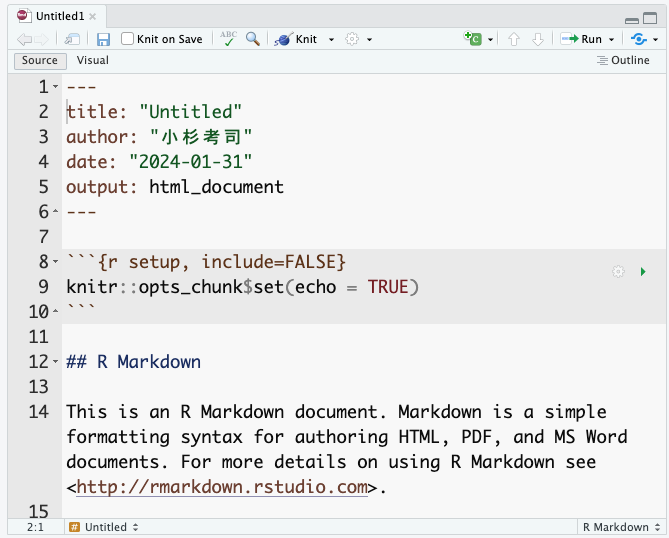
\includegraphics{../common/images/04_RmdSample.png}

}

\caption{Rmarkdownファイルのサンプル}

\end{figure}%%
\begin{figure}[H]

{\centering 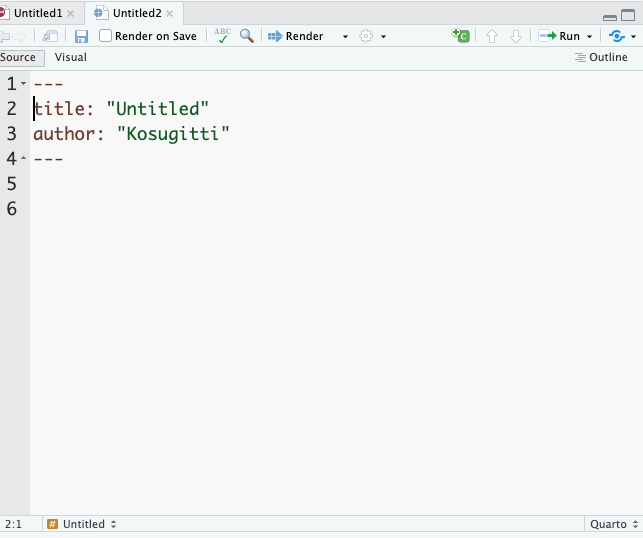
\includegraphics{../common/images/04_QmdSample.png}

}

\caption{Quartoファイルのサンプル}

\end{figure}%

Rmarkdown,Quartoともに,ファイルの冒頭に4つのハイフンで囲まれた領域が見て取れるだろう。これはYAMLヘッダ(YAMLはYet
Another Markup
Languageの略。ここはまだマークアップ領域じゃないよということ)と呼ばれる,文書全体に対する設定をする領域のことである。

この領域を一瞥すると,タイトルや著者名,出力形式などが記載されていることが見て取れる。YAMLヘッダはインデントに敏感で,また正しくない記述が含まれているとエラーになって出力ファイルが作られないことが少なくないため,ここを手動で書き換えるときは注意が必要である。とはいえ,ここを自在に書き換えることができるようになると,様々な応用が効くので興味があるものは調べて色々トライしてもらいたい。

さて,Rmd/Qmdのファイル上部にKnitあるいはRenderと書かれたボタンがあるだろう。これをクリックすると,表示用ファイルへの変換が実行される。\footnote{もし新しく開いているファイルに名前がつけられていないのなら(Untitledのままになっているようであれば),ファイル名の指定画面が開く。また環境によっては,初回実行時にコンパイルに必要な関連パッケージのダウンロードが求められることがある。}
Rmarkdownの場合は,すでにサンプルコードが含まれているので,数値および図表のはいったHTMLドキュメントが表示されるだろう。以下はこのサンプルコードを例に説明するため,Rmarkdownとそのコンパイル(knit))を一度試してもらいたい。その上で,元のRmdファイルと出来上がったファイルとの対応関係を確認してみよう。

\begin{figure}[H]

{\centering 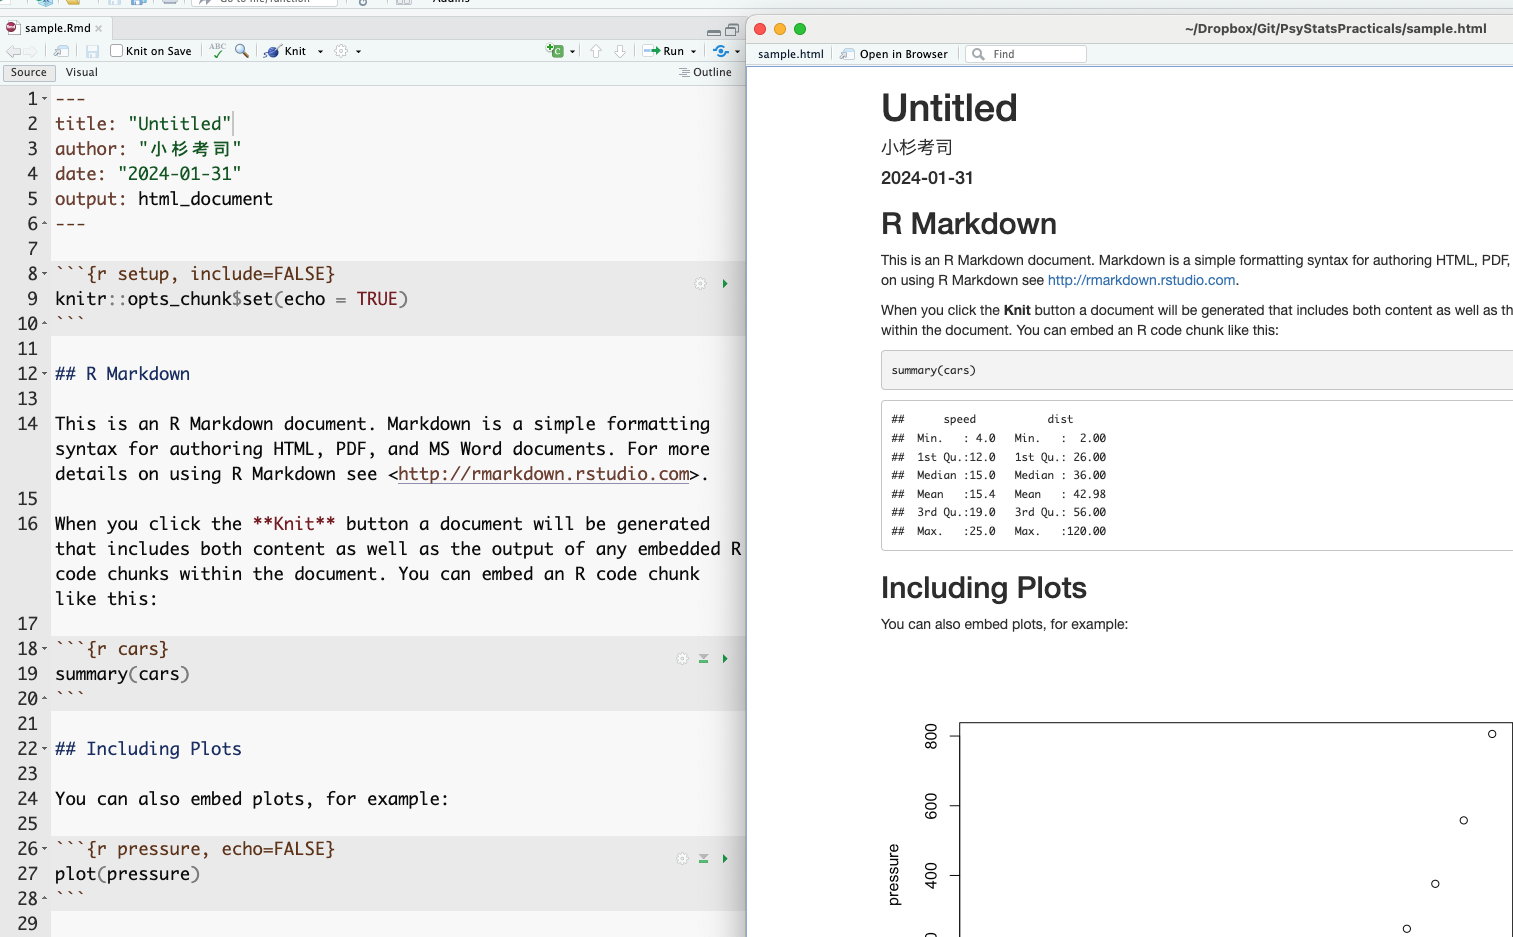
\includegraphics{../common/images/04_coresspRmd.png}

}

\caption{Rmdファイルと出力結果の対応}

\end{figure}%

おおよそ,何がどのように変換されているかの対応が推察できるだろう。
出力ファイルの冒頭には,YAMLで設定したタイトル,著者名,日付などが表示されているし,\texttt{\#}の印がついていた一行は見出しとして強調されている。

特に注目したいのが,元のファイルで3つのクォーテーションで囲まれた灰色の領域である。この領域のことを特に\textbf{チャンク}といい,ここに書かれたRスクリプトが変換時に実行され,結果として出力される。出力ファイルをみると,\texttt{summary(cars)}
というチャンクで指定された命令文があり,その結果(carsというデータセットの要約)が出力されているのが見て取れる。繰り返しになるが,ポイントは原稿ファイルには計算を指示するスクリプトが書かれているだけで,出力結果を書いていないことにある。原稿は指示だけなのである。こうすることで,コピー&ペーストのミスがなくなるし,同じRmd/Qmd原稿とデータを持っていれば,ことなるPC上でも同じ出力が得られる。環境を統合することで,ミスの防止と再現可能性に貢献しているのがわかるだろう。

今回は\texttt{cars}というRがデフォルトでもっているサンプルデータの例なので,どの環境でも同じ結果が出力されている。しかしもちろん,個別のデータファイルであっても,同じファイルで同じ読み込み方,同じ加工をしていれば,環境が違っても追跡可能である。注意して欲しいのは,コンパイルするときは新しい環境から行われるという点ある。すなわち,\textbf{原稿ファイルにないオブジェクトの利用はできない}のである。これは再現性を担保するという意味では当然のことで,「事前に別途処理しておいたデータ」から分析を始められても,その事前処理が適切だったかどうかがチェックできないからである。Rmd/Qmdファイルと,CSVファイルなどの素データが共有されていれば再現できる,という利点を活かすため,データハンドリングを含めた前処理も全てチャンクに書き込み,新しい環境で最初からトレースできるようにする必要がある。不便に感じるところもあるかもしれないが,科学的営みとして重要な手続きであることを理解してもらいたい。\footnote{もっとも,Rのバージョンやパッケージのバージョンによっては同じ計算結果が出ない可能性がある。より本質的な計算過程に違いがあるかもしれないのである。そのため,R本体やパッケージのバージョンごとパッキングして共有する工夫も考えられている。Dockerと呼ばれるシステムは,解析環境ごと保全し共有するシステムの例である。}

RStudiでは,ビジュアルモードやアウトライン表示,チャンク挿入ボタンやチャンクごとの実行・設定などRmd/Qmdファイルの編集に便利な機能も複数用意されているので,
\textcite{Takahashi201805} などを参考にいろいろ試してみるといいだろう。

\subsection{マークダウンの記法}\label{ux30deux30fcux30afux30c0ux30a6ux30f3ux306eux8a18ux6cd5}

以下では,マークダウン記法について基本的な利用法を解説する。

\subsubsection{見出しと強調}\label{ux898bux51faux3057ux3068ux5f37ux8abf}

すでに見たように,マークダウンでは\texttt{\#}記号で見出しを作ることができる。\texttt{\#}の数が見出しレベルに対応し,\texttt{\#}はトップレベル,本でいうところの「章,chapter」,HTMLでいうところの\texttt{H1}に相当する。\texttt{\#}記号の後ろに半角スペースが必要なことに注意されたし。以下,\texttt{\#\#}で「節,section」あるいは\texttt{H2},\texttt{\#\#\#}で小節(subsection,\texttt{H3}),\texttt{\#\#\#\#}で小小節(subsubsection,\texttt{H4})\ldots と続く。

心理学を始め,科学論文の書き方としての「パラグラフライティング」を既にみしっていることだろう。文章をセクション,サブセクション,パラグラフ,センテンスのように階層的に分割し,それぞれの区分が4つの下位区分を含むような文章構造である。心理学の場合は特に「問題,方法,結果,考察」の4セクションで一論文が構成されるのが基本である。こうしたアウトラインを意識した書き方は読み手にも優しく,マークダウンの記法ではそれが自然と実装できるようになっている。

これとは別に,一部を太字や斜体で強調したいこともあるだろう。そのような場合はアスタリスクを1つ,あるいは2つつけて\emph{強調}したり\textbf{強調}したりできる。

\subsubsection{図表とリンク}\label{ux56f3ux8868ux3068ux30eaux30f3ux30af}

文中に図表を挿入したいこともあるだろう。表の挿入は,マークダウン独自の記法があり,縦棒\texttt{\textbar{}}やハイフン\texttt{-}を駆使して以下のように表記する。

\begin{verbatim}
| Header 1 | Header 2 | Header 3 |
| -------- | -------- | -------- |
| Row 1    | Data 1   | Data 2   |
| Row 2    | Data 3   | Data 4   |
\end{verbatim}

Rのコードの中には分析結果をマークダウン形式で出力してくれる関数もあるし,表計算ソフトなどでできた表があるなら,chatGPTなど生成AIを利用するとすぐに書式変換してくれるので,そういったツールを活用すると良い。

図の挿入は,マークダウンでは図のファイルへのリンクと考えると良い。次のように,大括弧で括った文字がキャプション,つづく小括弧で括ったものが図へのリンクとなる。実際に表示されるときは図が示される。

\begin{verbatim}
![図のキャプション](図へのリンク)
\end{verbatim}

同様に,ウェブサイトへのリンクなども,\texttt{{[}表示名{]}(リンク先)}の書式で対応できる。

\subsubsection{リスト}\label{ux30eaux30b9ux30c8}

並列的に箇条書きを示したい場合は,プラスあるいはマイナスでリストアップする。注意すべきは,リストの前後に改行を入れておくべきことである。

\begin{verbatim}
ここまで前の文

+  list item 1
+  list item 2
+  list item 3
    - sub item 1
    - sub item 2

ここから次の文
\end{verbatim}

\subsubsection{チャンク}\label{ux30c1ux30e3ux30f3ux30af}

既に述べたように,チャンク(chunk)と呼ばれる領域は実行されるコードを記載するところである。チャンクはまず,バックスラッシュ3つ繋げることでコードブロックであることを示し,次に
\texttt{r}と書くことで計算エンジンがRであることを明示する。ここにJuiliaやPythonなど他の計算エンジンを指定することも可能である。

可能であれば,チャンク名をつけておくと良い。次の例は,チャンク名として「chunksample」を与えたものである。チャンク名をつけておくと,RStudioでは見出しジャンプをつかって移動することもできるので,編集時に便利である。

```\{r chunksample,echo = FALSE\} summary(cars) ```

さらに,\texttt{echo\ =\ FALSE}のようにチャンクオプションを指定することができる。\texttt{echo=FALSE}は入力したスクリプトを表示せず,結果だけにするオプションである。そのほか「計算結果を含めない」「表示せずに計算は実行する」等様々な指定が可能である。

なおQuartoではこのチャンクオプションを次のように書くこともできる。

```\{r\} \#\textbar{} echo: FALSE \#\textbar{} include: FALSE
summary(cars) ```

\section{プロットによる基本的な描画}\label{ux30d7ux30edux30c3ux30c8ux306bux3088ux308bux57faux672cux7684ux306aux63cfux753b}

再現可能な文書という観点から,図表もスクリプトによる記述で表現することは重要である。

\textbf{データはまず可視化するもの}と心がけよ。可視化は,数値の羅列あるいはまとめられた統計量では把握しきれない多くの情報を提供し,潜在的な関係性を直観的に見つけ出せる可能性がある。なので,取得したあらゆる\textbf{データはまず可視化するもの},と思っておいて間違いはない。大事なことなので二度言いました。可視化の重要性については心理学の知見にも触れている
\textcite{Kieran2018} も参考にしてほしい。

さて,Rには基本的な作図環境も整っており,\texttt{plot}という関数に引数として,x軸,y軸に相当する変数を与えるだけで,簡単に散布図を書いてくれる。

\begin{Shaded}
\begin{Highlighting}[]
\FunctionTok{plot}\NormalTok{(iris}\SpecialCharTok{$}\NormalTok{Sepal.Length, iris}\SpecialCharTok{$}\NormalTok{Sepal.Width,}
  \AttributeTok{main =} \StringTok{"Example of Scatter Plot"}\NormalTok{,}
  \AttributeTok{xlab =} \StringTok{"Sepal.Length"}\NormalTok{,}
  \AttributeTok{ylab =} \StringTok{"Sepal.Width"}
\NormalTok{)}
\end{Highlighting}
\end{Shaded}

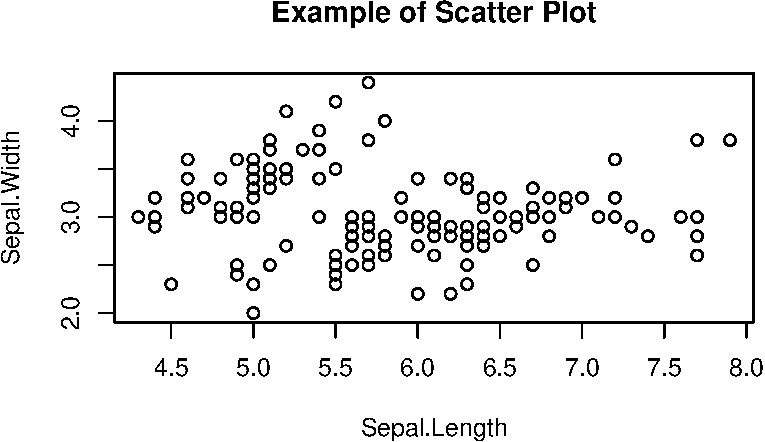
\includegraphics{chapter04_files/figure-pdf/RplotSample-1.pdf}

この関数のオプションとして,タイトルを与えたり,軸に名前を与えたりできる。またプロットされるピンの形,描画色,背景色など様々な操作が可能である。特段のパッケージを必要とせずとも,基本的な描画機能は備えていると言えるだろう。

\section{ggplotによる描画}\label{ggplotux306bux3088ux308bux63cfux753b}

ここでは,\texttt{tidyverse}に含まれる描画専用のパッケージである,\texttt{ggplot2}
パッケージを用いた描画を学ぶ。Rの基本描画関数でもかなりのことができるのだが,この\texttt{ggplot2}パッケージをもちいた図の方が美しく,直観的に操作できる。というのも\texttt{ggplot}の\texttt{gg}とは\texttt{The\ Grammar\ of\ Graphics}(描画の文法)のことであり,このことが示すようにロジカルに図版を制御できるからである。\texttt{ggplot2}の形で記述された図版のスクリプトは可読性が高く,視覚的にも美しいため,多くの文献で利用されている。

\texttt{ggplot2}
パッケージの提供する描画環境の特徴は,レイア(Layer)の概念である。図版は複数のレイアの積み重ねとして表現される。まず土台となるキャンバスがあり,そこにデータセット,幾何学的オブジェクト(点,線,バーなど),エステティックマッピング(色,形,サイズなど),凡例やキャプションを重ねていく,という発想である。そして図版全体を通したテーマを手強することで,カラーパレットの統一などの仕上げをすれば,すぐにでも論文投稿可能なレベルの図版を描くことができる。

以下に\texttt{ggplot2}における描画のサンプルを示す。サンプルデータ\texttt{mtcars}を用いた。

\begin{Shaded}
\begin{Highlighting}[]
\FunctionTok{library}\NormalTok{(ggplot2)}

\FunctionTok{ggplot}\NormalTok{(}\AttributeTok{data =}\NormalTok{ mtcars, }\FunctionTok{aes}\NormalTok{(}\AttributeTok{x =}\NormalTok{ wt, }\AttributeTok{y =}\NormalTok{ mpg)) }\SpecialCharTok{+}
  \FunctionTok{geom\_point}\NormalTok{() }\SpecialCharTok{+}
  \FunctionTok{geom\_smooth}\NormalTok{(}\AttributeTok{method =} \StringTok{"lm"}\NormalTok{, }\AttributeTok{formula =} \StringTok{"y \textasciitilde{} x"}\NormalTok{) }\SpecialCharTok{+}
  \FunctionTok{labs}\NormalTok{(}\AttributeTok{title =} \StringTok{"車の重量と燃費の関係"}\NormalTok{, }\AttributeTok{x =} \StringTok{"重量"}\NormalTok{, }\AttributeTok{y =} \StringTok{"燃費"}\NormalTok{)}
\end{Highlighting}
\end{Shaded}

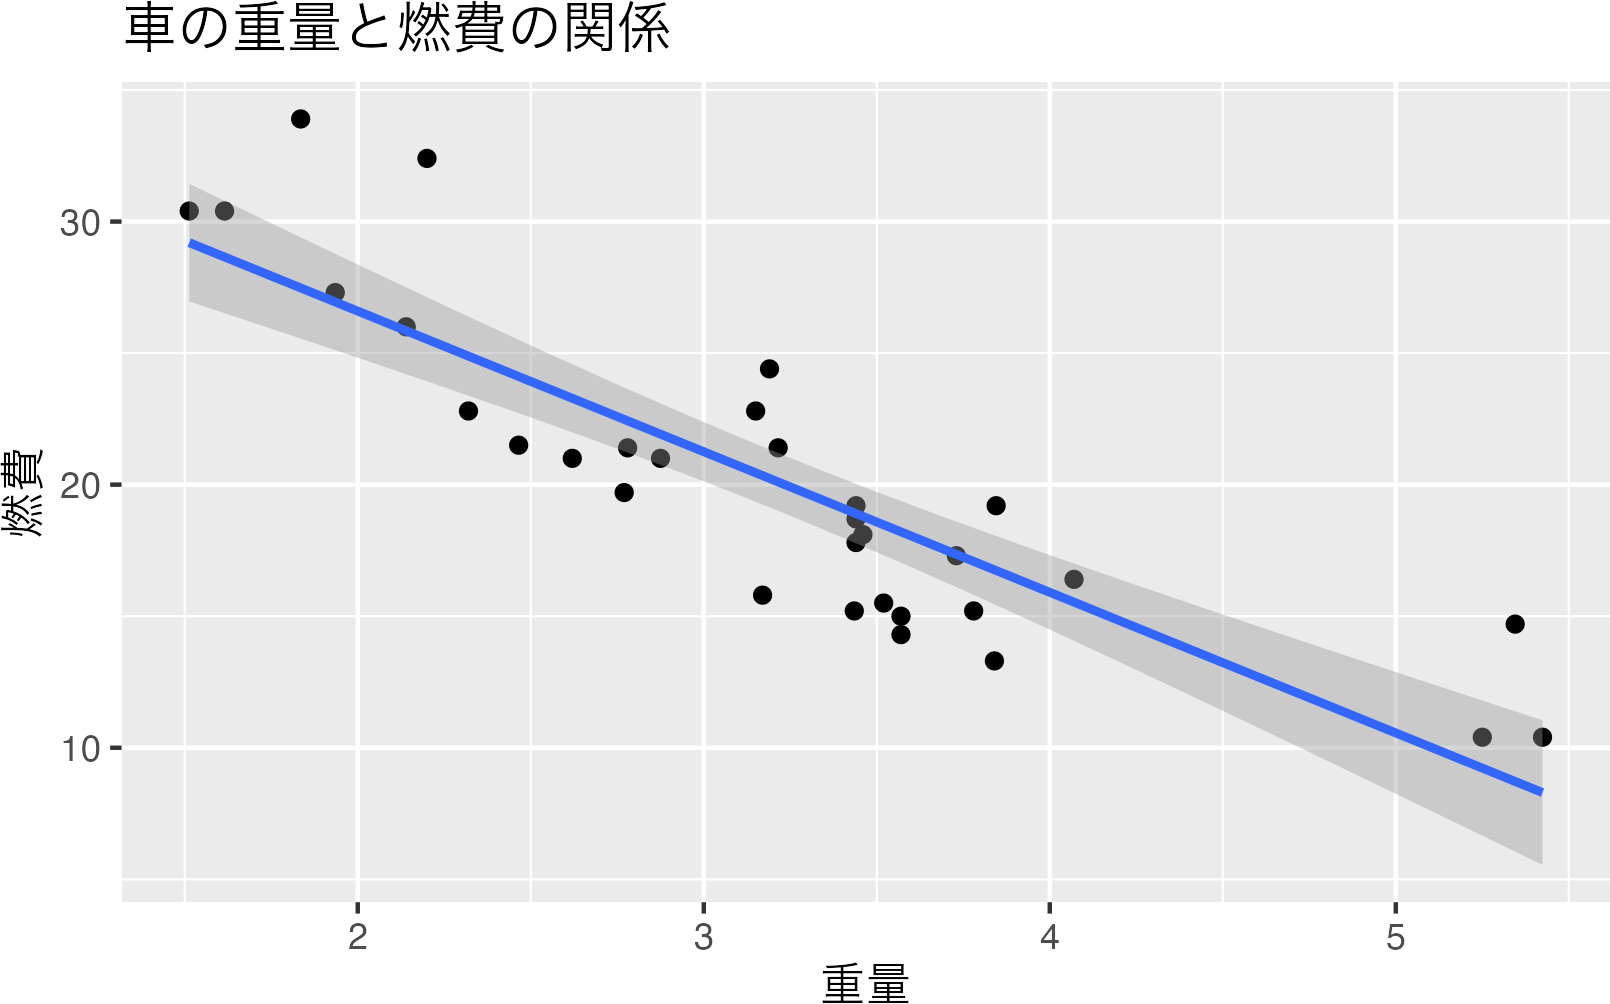
\includegraphics{chapter04_files/figure-pdf/ggplotSample1-1.png}

まずは出来上がる図版の美しさと,コードのイメージを把握してもらいたい。
最初の\texttt{library(ggplot2)}はパッケージを読み込んでいるところである。今回は明示的に\texttt{ggplot2}を読み込んでいるが,\texttt{tidyverse}パッケージを読み込むと同時に読み込まれているので,Rのスクリプトの冒頭に\texttt{library(tidyverse)}と書く癖をつけておけば必要ない。

続いて\texttt{ggplot}の関数が4行にわたって書いてあるが,それぞれが\texttt{+}の記号で繋がれていることがわかるだろう。これがレイアを重ねるという作業に相当する。まずは,図を書くためのキャンバスを用意し,その上にいろいろ重ねていくのである。

次のコードは,キャンバスだけを描画した例である。

\begin{Shaded}
\begin{Highlighting}[]
\NormalTok{g }\OtherTok{\textless{}{-}} \FunctionTok{ggplot}\NormalTok{()}
\FunctionTok{print}\NormalTok{(g)}
\end{Highlighting}
\end{Shaded}


\includegraphics{chapter04_files/figure-pdf/canvasOnly-1.pdf}

ここでは\texttt{g}
というオブジェクトを\texttt{ggplot}関数でつくり,それを表示させた。最初はこのようにプレーンなキャンバスだが,ここに次々と上書きしていくことになる。

\section{幾何学的オブジェクトgeom}\label{ux5e7eux4f55ux5b66ux7684ux30aaux30d6ux30b8ux30a7ux30afux30c8geom}

幾何学的オブジェクト(geometric object)
とは,データの表現方法の指定であり,\texttt{ggplot}には様々なパターンが用意されている。以下に一例を挙げる。

\begin{itemize}
\tightlist
\item
  \textbf{\texttt{geom\_point()}}:
  散布図で使用され、データ点を個々の点としてプロットする。
\item
  \textbf{\texttt{geom\_line()}}:
  折れ線グラフで使用され、データ点を線で結んでプロットする。時系列データなどによく使われる。
\item
  \textbf{\texttt{geom\_bar()}}:
  棒グラフで使用され、カテゴリごとの量を棒で表示する。データの集計(カウントや合計など)に適している。
\item
  \textbf{\texttt{geom\_histogram()}}:
  ヒストグラムで使用され、連続データの分布を棒で表示する。データの分布を理解するのに役立つ。
\item
  \textbf{\texttt{geom\_boxplot()}}:
  箱ひげ図で使用され、データの分布(中央値、四分位数、外れ値など)を要約して表示する。
\item
  \textbf{\texttt{geom\_smooth()}}:
  平滑化曲線を追加し、データのトレンドやパターンを可視化する。線形回帰やローパスフィルタなどの方法が使われる。
\end{itemize}

これらの幾何学的オブジェクトに,データおよび軸との対応を指定するなどして描画する。次に挙げるのは\texttt{geom\_point}
による点描画,つまり散布図である。

\begin{Shaded}
\begin{Highlighting}[]
\FunctionTok{ggplot}\NormalTok{() }\SpecialCharTok{+}
  \FunctionTok{geom\_point}\NormalTok{(}\AttributeTok{data =}\NormalTok{ mtcars, }\AttributeTok{mapping =} \FunctionTok{aes}\NormalTok{(}\AttributeTok{x =}\NormalTok{ disp, }\AttributeTok{y =}\NormalTok{ wt))}
\end{Highlighting}
\end{Shaded}

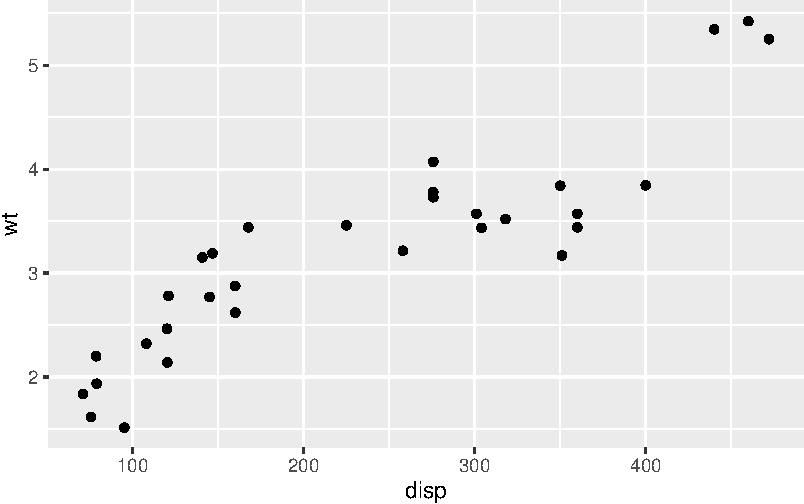
\includegraphics{chapter04_files/figure-pdf/geom_exam-1.pdf}

一行目でキャンバスを用意し,そこに\texttt{geom\_point}で点を打つようにしている。
このとき,データは\texttt{mtcars}であり,x軸に変数\texttt{disp}を,y軸に変数\texttt{wt}をマッピングしている。マッピング関数の\texttt{aes}はaesthetic
mappingsの意味で,データによって変わる値(x座標,y座標,色,サイズ,透明度など)を指定することができる。

レイアは次々と重ねることができる。以下の例を見てみよう。

\begin{Shaded}
\begin{Highlighting}[]
\NormalTok{g }\OtherTok{\textless{}{-}} \FunctionTok{ggplot}\NormalTok{()}
\NormalTok{g1 }\OtherTok{\textless{}{-}}\NormalTok{ g }\SpecialCharTok{+} \FunctionTok{geom\_point}\NormalTok{(}\AttributeTok{data =}\NormalTok{ mtcars, }\AttributeTok{mapping =} \FunctionTok{aes}\NormalTok{(}\AttributeTok{x =}\NormalTok{ disp, }\AttributeTok{y =}\NormalTok{ wt))}
\NormalTok{g2 }\OtherTok{\textless{}{-}}\NormalTok{ g1 }\SpecialCharTok{+} \FunctionTok{geom\_line}\NormalTok{(}\AttributeTok{data =}\NormalTok{ mtcars, }\AttributeTok{mapping =} \FunctionTok{aes}\NormalTok{(}\AttributeTok{x =}\NormalTok{ disp, }\AttributeTok{y =}\NormalTok{ wt))}
\FunctionTok{print}\NormalTok{(g2)}
\end{Highlighting}
\end{Shaded}

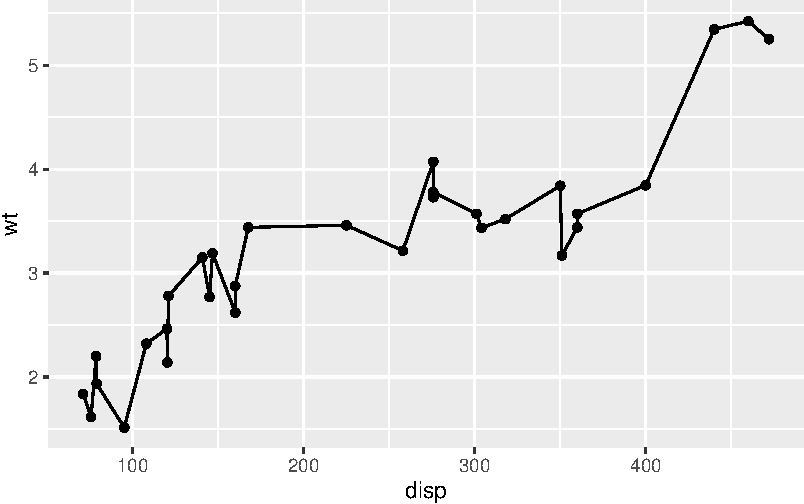
\includegraphics{chapter04_files/figure-pdf/geom_overlay-1.pdf}

重ねることを強調するために,\texttt{g}
オブジェクトを次々作るようにしたが,もちろん1つのオブジェクトでまとめて書いてもいいし,\texttt{g}オブジェクトとして保管せずとも,最初の例のように直接出力することもできる。また,ここでは点描画オブジェクトに線描画オブジェクトを重ねているが,データやマッピングは全く同じである。異なるデータを一枚のキャンバスに書く場合は,このように幾何学オブジェクトごとの指定が可能であるが,図版は得てして一枚のキャンバスに一種類のデータになりがちである。そのような場合は,以下に示すようにキャンバスの段階から基本となるデータセットとマッピングを与えることが可能である。

\begin{Shaded}
\begin{Highlighting}[]
\FunctionTok{ggplot}\NormalTok{(}\AttributeTok{data =}\NormalTok{ mtcars, }\AttributeTok{mapping =} \FunctionTok{aes}\NormalTok{(}\AttributeTok{x =}\NormalTok{ disp, }\AttributeTok{y =}\NormalTok{ wt)) }\SpecialCharTok{+}
  \FunctionTok{geom\_point}\NormalTok{() }\SpecialCharTok{+}
  \FunctionTok{geom\_line}\NormalTok{()}
\end{Highlighting}
\end{Shaded}

また,この用例の場合\texttt{ggplot}関数の第一引数はデータセットなので,パイプ演算子で渡すことができる。

\begin{Shaded}
\begin{Highlighting}[]
\NormalTok{mtcars }\SpecialCharTok{\%\textgreater{}\%}
  \FunctionTok{ggplot}\NormalTok{(}\AttributeTok{mapping =} \FunctionTok{aes}\NormalTok{(}\AttributeTok{x =}\NormalTok{ disp, }\AttributeTok{y =}\NormalTok{ wt)) }\SpecialCharTok{+}
  \FunctionTok{geom\_point}\NormalTok{() }\SpecialCharTok{+}
  \FunctionTok{geom\_line}\NormalTok{()}
\end{Highlighting}
\end{Shaded}

パイプ演算子を使うことで,素データをハンドリングし,必要な形に整えて可視化する,という流れがスクリプト上で読むように表現できるようになる。慣れてくると,データセットから可視化したい要素を特定し,最終的にどのように成形すれば\texttt{ggplot}に渡しやすくなるかを想像して加工していくようになる。そのためには到達目標となる図版のイメージを頭に描き,その図のx軸,y軸は何で,どのような幾何学オブジェクトが上に乗っているのか,といったように図版のリバースエンジニアリング,あるいは図版の作成手順の書き下しができる必要がある。たとえるなら,食べたい料理に必要な材料を集め,大まかな手順(下ごしらえからの調理)を組み立てられるかどうか,である。実際にレシピに書き起こす際は生成AIの力を借りると良いが,その際も最終的な目標と,全体的な設計方針から指示し,微調整を追加していくように指示すると効率的である。

以下に,データハンドリングと描画の一例を示す。各ステップにコメントをつけたので,文章を読むように加工と描画の流れを確認し,出力結果と照らし合わせてみよう。

\begin{Shaded}
\begin{Highlighting}[]
\CommentTok{\# mtcarsデータセットを使用}
\NormalTok{mtcars }\SpecialCharTok{\%\textgreater{}\%}
  \CommentTok{\# 変数選択}
  \FunctionTok{select}\NormalTok{(mpg, cyl, wt, am) }\SpecialCharTok{\%\textgreater{}\%}
  \FunctionTok{mutate}\NormalTok{(}
    \CommentTok{\# 変数am,cylをFactor型に変換}
    \AttributeTok{am =} \FunctionTok{factor}\NormalTok{(am, }\AttributeTok{labels =} \FunctionTok{c}\NormalTok{(}\StringTok{"automatic"}\NormalTok{, }\StringTok{"manual"}\NormalTok{)),}
    \AttributeTok{cyl =} \FunctionTok{factor}\NormalTok{(cyl)}
\NormalTok{  ) }\SpecialCharTok{\%\textgreater{}\%}
  \CommentTok{\# 水準ごとにグループ化}
  \FunctionTok{group\_by}\NormalTok{(am, cyl) }\SpecialCharTok{\%\textgreater{}\%}
  \FunctionTok{summarise}\NormalTok{(}
    \AttributeTok{M =} \FunctionTok{mean}\NormalTok{(mpg), }\CommentTok{\# 各グループの平均燃費(M)を計算}
    \AttributeTok{SD =} \FunctionTok{sd}\NormalTok{(mpg), }\CommentTok{\# 各グループの燃費の標準偏差(SD)を計算}
    \AttributeTok{.groups =} \StringTok{"drop"} \CommentTok{\# summarise後の自動的なグルーピングを解除}
\NormalTok{  ) }\SpecialCharTok{\%\textgreater{}\%}
  \CommentTok{\# x軸にトランスミッションの種類、y軸に平均燃費,塗りつぶしの色はcyl}
  \FunctionTok{ggplot}\NormalTok{(}\FunctionTok{aes}\NormalTok{(}\AttributeTok{x =}\NormalTok{ am, }\AttributeTok{y =}\NormalTok{ M, }\AttributeTok{fill =}\NormalTok{ cyl)) }\SpecialCharTok{+}
  \CommentTok{\# 横並びの棒グラフ}
  \FunctionTok{geom\_bar}\NormalTok{(}\AttributeTok{stat =} \StringTok{"identity"}\NormalTok{, }\AttributeTok{position =} \StringTok{"dodge"}\NormalTok{) }\SpecialCharTok{+}
  \CommentTok{\# ±1SDのエラーバーを追加}
  \FunctionTok{geom\_errorbar}\NormalTok{(}
    \CommentTok{\# エラーバーのマッピング}
    \FunctionTok{aes}\NormalTok{(}\AttributeTok{ymin =}\NormalTok{ M }\SpecialCharTok{{-}}\NormalTok{ SD, }\AttributeTok{ymax =}\NormalTok{ M }\SpecialCharTok{+}\NormalTok{ SD),}
    \CommentTok{\# エラーバーの位置を棒グラフに合わせる}
    \AttributeTok{position =} \FunctionTok{position\_dodge}\NormalTok{(}\AttributeTok{width =} \FloatTok{0.9}\NormalTok{),}
    \AttributeTok{width =} \FloatTok{0.25} \CommentTok{\# エラーバーの幅を設定}
\NormalTok{  )}
\end{Highlighting}
\end{Shaded}

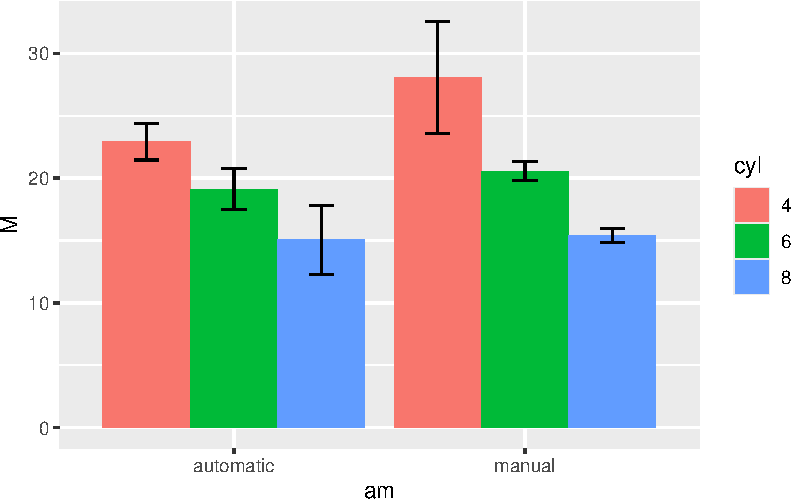
\includegraphics{chapter04_files/figure-pdf/withHandlingGGplot-1.pdf}

繰り返しになるが,このコードは慣れてくるまでいきなり書けるものではない。重要なのは「出力結果をイメージ」することと,それを「要素に分解」,「手順に沿って並べる」ことができるかどうかである。\footnote{実際コードはchatGPTver4に指示して生成した。いきなり全体像を描くのではなく,徐々に追記していくと効果的である。}

\section{描画tips}\label{ux63cfux753btips}

最後に,いくつかの描画テクニックを述べておく。これらについては,必要な時に随時ウェブ上で検索したり,生成AIに尋ねることでも良いが,このような方法がある,という基礎知識を持っておくことも重要だろう。なお描画について詳しくは
\textcite{Kinosady2021} の4章を参照すると良い。

\subsection{ggplotオブジェクトを並べる}\label{ggplotux30aaux30d6ux30b8ux30a7ux30afux30c8ux3092ux4e26ux3079ux308b}

複数のプロットを一枚のパネルに配置したい,ということがあるかもしれない。先ほどの\texttt{mtcars}データの例でいえば,\texttt{am}変数にオートマチック車かマニュアル車かの2水準があるが,このようなサブグループごとに図を分割したいという場合である。

このような時には,\texttt{facet\_wrap}や\texttt{facet\_grid}という関数が便利である。前者はある変数について,後者は2つの変数について図を分割する。

\begin{Shaded}
\begin{Highlighting}[]
\NormalTok{mtcars }\SpecialCharTok{\%\textgreater{}\%}
  \CommentTok{\# 重さwtと燃費mpgの散布図}
  \FunctionTok{ggplot}\NormalTok{(}\FunctionTok{aes}\NormalTok{(}\AttributeTok{x =}\NormalTok{ wt, }\AttributeTok{y =}\NormalTok{ mpg)) }\SpecialCharTok{+}
  \FunctionTok{geom\_point}\NormalTok{() }\SpecialCharTok{+}
  \CommentTok{\# シリンダ数cylで分割}
  \FunctionTok{facet\_wrap}\NormalTok{(}\SpecialCharTok{\textasciitilde{}}\NormalTok{cyl, }\AttributeTok{nrow =} \DecValTok{2}\NormalTok{) }\SpecialCharTok{+}
  \CommentTok{\# タイトルをつける}
  \FunctionTok{labs}\NormalTok{(}\AttributeTok{caption =} \StringTok{"facet\_wrapの例"}\NormalTok{)}
\end{Highlighting}
\end{Shaded}

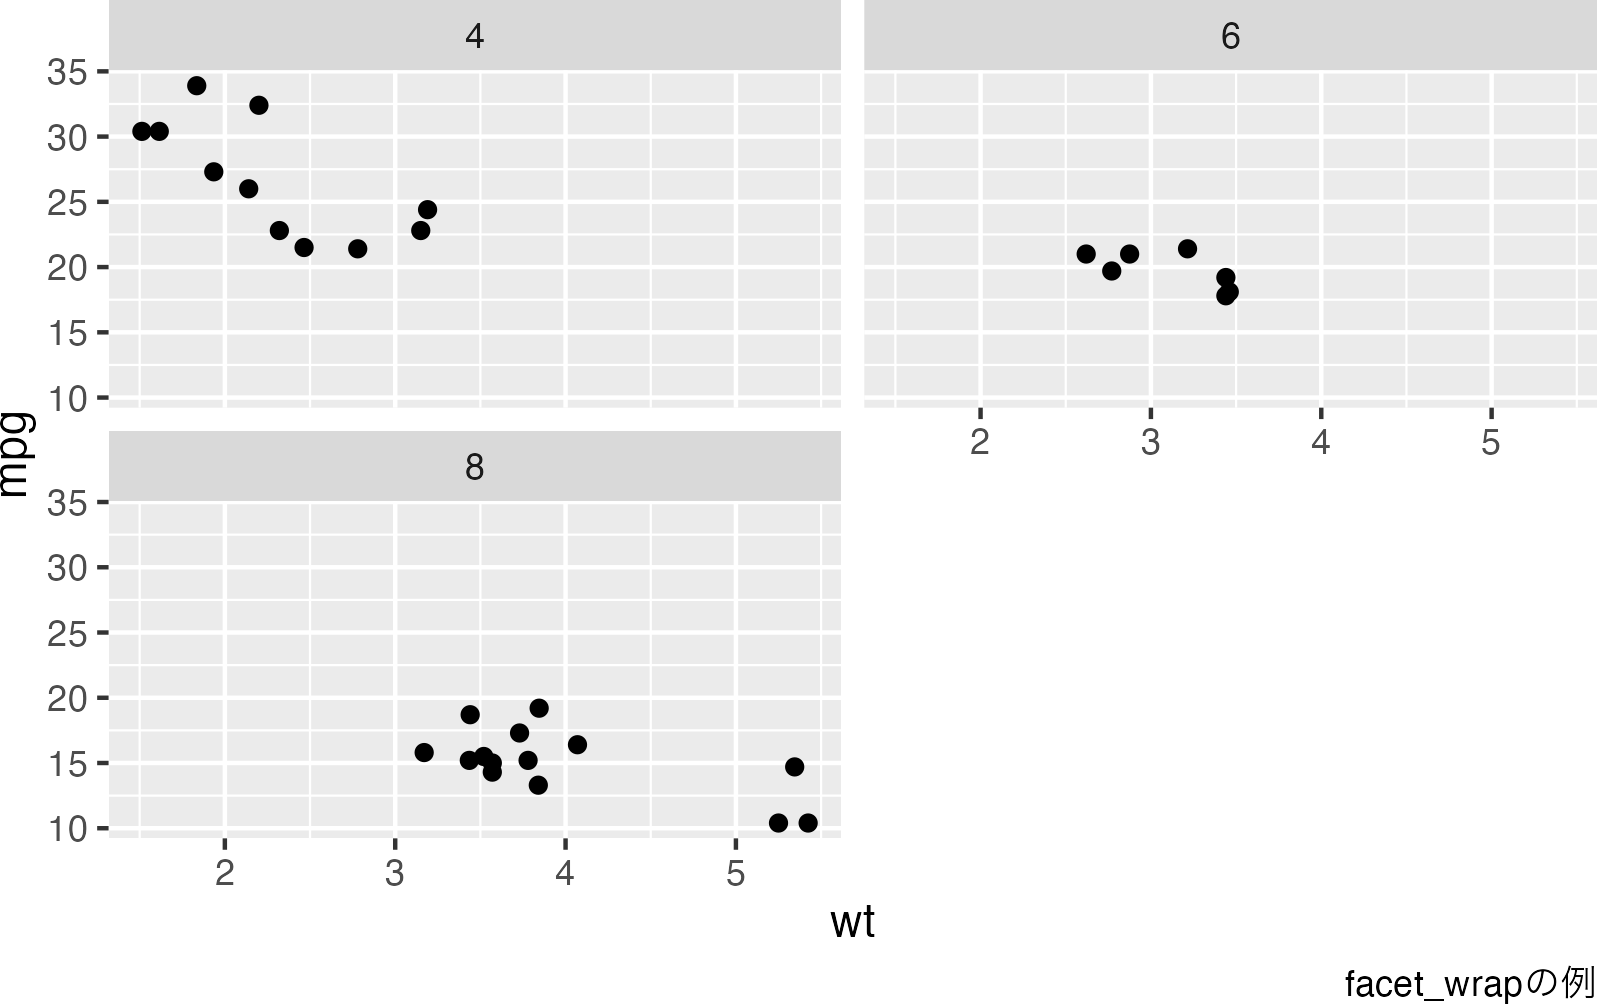
\includegraphics{chapter04_files/figure-pdf/exampleFacetWrap-1.png}

\begin{Shaded}
\begin{Highlighting}[]
\NormalTok{mtcars }\SpecialCharTok{\%\textgreater{}\%}
  \FunctionTok{ggplot}\NormalTok{(}\FunctionTok{aes}\NormalTok{(}\AttributeTok{x =}\NormalTok{ wt, }\AttributeTok{y =}\NormalTok{ mpg)) }\SpecialCharTok{+}
  \FunctionTok{geom\_point}\NormalTok{() }\SpecialCharTok{+}
  \CommentTok{\# シリンダ数cylとギア数gearで分割}
  \FunctionTok{facet\_grid}\NormalTok{(cyl }\SpecialCharTok{\textasciitilde{}}\NormalTok{ gear) }\SpecialCharTok{+}
  \CommentTok{\# キャプションをつける}
  \FunctionTok{labs}\NormalTok{(}\AttributeTok{caption =} \StringTok{"facet\_gridの例"}\NormalTok{)}
\end{Highlighting}
\end{Shaded}

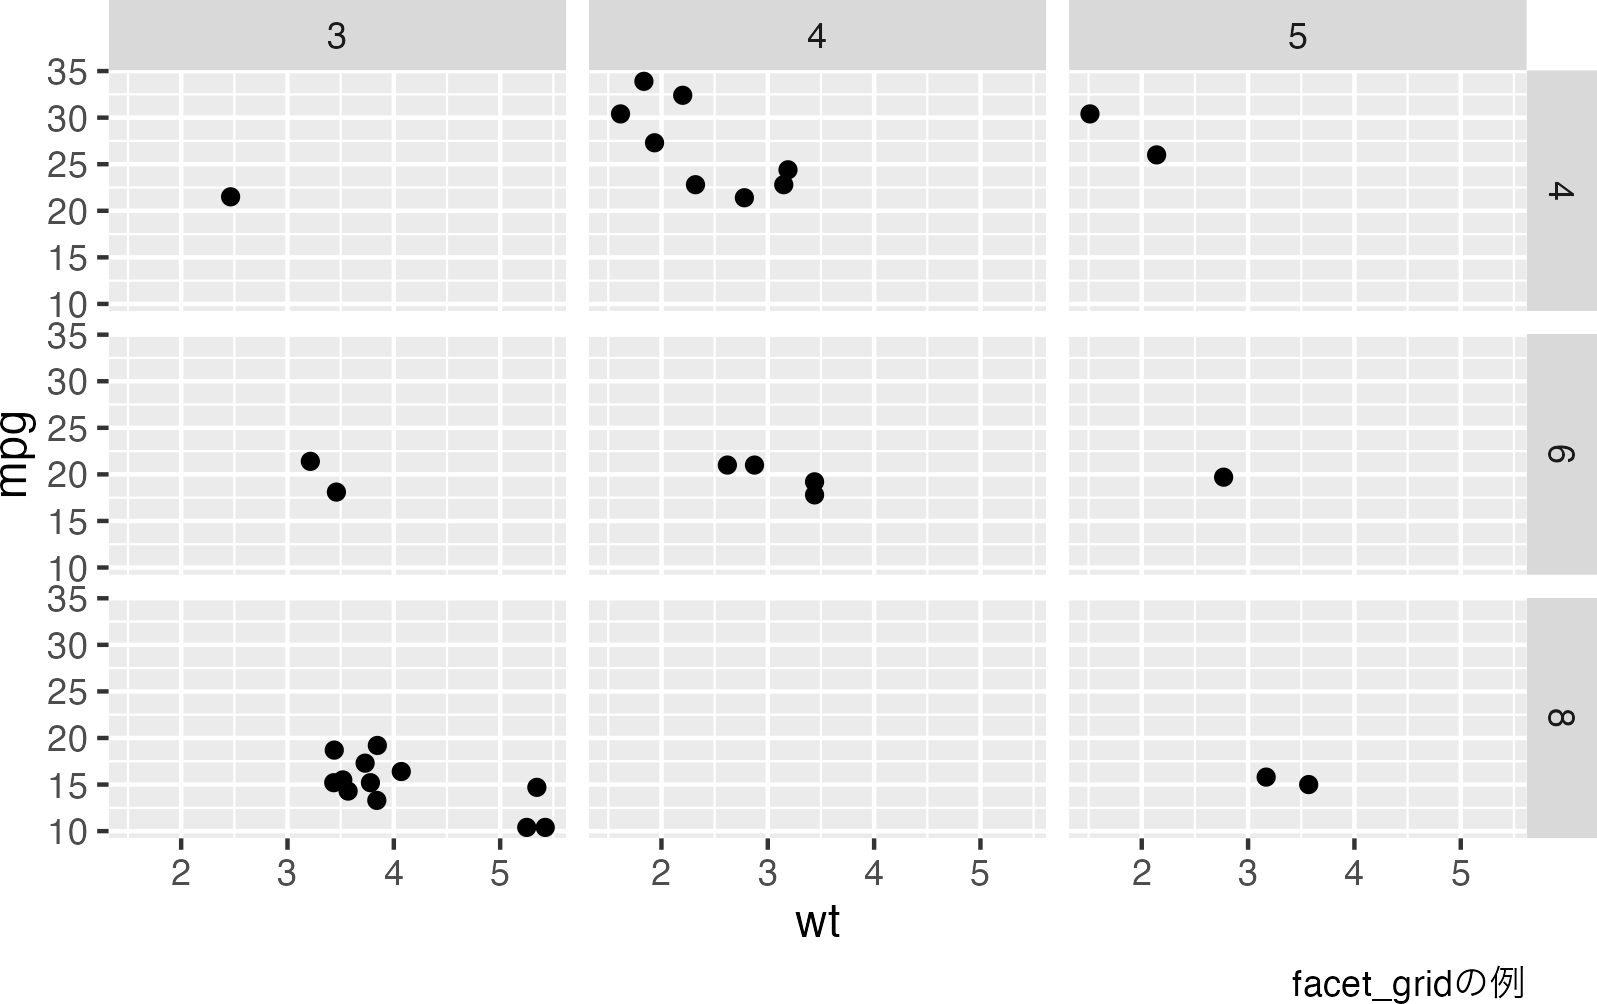
\includegraphics{chapter04_files/figure-pdf/exampleFacetGrid-1.png}

一枚の図をサブグループに分けるのではなく,異なる図を一枚の図として赤痛いこともあるかもしれない。そのような場合は,\texttt{patchwork}パッケージを使うと便利である。

\begin{Shaded}
\begin{Highlighting}[]
\FunctionTok{library}\NormalTok{(patchwork)}

\CommentTok{\# 散布図の作成}
\NormalTok{g1 }\OtherTok{\textless{}{-}} \FunctionTok{ggplot}\NormalTok{(mtcars, }\FunctionTok{aes}\NormalTok{(}\AttributeTok{x =}\NormalTok{ wt, }\AttributeTok{y =}\NormalTok{ mpg)) }\SpecialCharTok{+}
  \FunctionTok{geom\_point}\NormalTok{() }\SpecialCharTok{+}
  \CommentTok{\# 散布図のタイトルとサブタイトル}
  \FunctionTok{ggtitle}\NormalTok{(}\StringTok{"Scatter Plot"}\NormalTok{, }\StringTok{"MPG vs Weight"}\NormalTok{)}

\CommentTok{\# 棒グラフの作成}
\NormalTok{g2 }\OtherTok{\textless{}{-}} \FunctionTok{ggplot}\NormalTok{(mtcars, }\FunctionTok{aes}\NormalTok{(}\AttributeTok{x =} \FunctionTok{factor}\NormalTok{(cyl), }\AttributeTok{y =}\NormalTok{ mpg)) }\SpecialCharTok{+}
  \FunctionTok{geom\_bar}\NormalTok{(}\AttributeTok{stat =} \StringTok{"identity"}\NormalTok{) }\SpecialCharTok{+}
  \CommentTok{\# 棒グラフのタイトルとサブタイトル}
  \FunctionTok{ggtitle}\NormalTok{(}\StringTok{"Bar Chart"}\NormalTok{, }\StringTok{"Average MPG by Cylinder"}\NormalTok{)}

\CommentTok{\# patchworkを使用して2つのグラフを組み合わせる}
\NormalTok{combined\_plot }\OtherTok{\textless{}{-}}\NormalTok{ g1 }\SpecialCharTok{+}\NormalTok{ g2 }\SpecialCharTok{+}
  \FunctionTok{plot\_annotation}\NormalTok{(}
    \AttributeTok{title =} \StringTok{"Combined Plots"}\NormalTok{,}
    \AttributeTok{subtitle =} \StringTok{"Scatter and Bar Charts"}
\NormalTok{  )}

\CommentTok{\# プロットを表示}
\FunctionTok{print}\NormalTok{(combined\_plot)}
\end{Highlighting}
\end{Shaded}

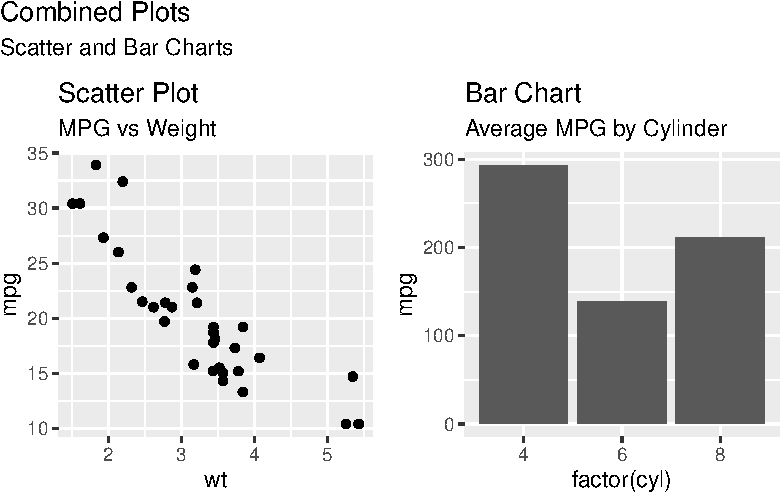
\includegraphics{chapter04_files/figure-pdf/patchwork example-1.pdf}

\subsection{ggplotオブジェクトの保存}\label{ggplotux30aaux30d6ux30b8ux30a7ux30afux30c8ux306eux4fddux5b58}

RmdやQuartoで文書を作るときは,図が自動的に生成されるので問題ないが,図だけ別のファイルとして利用したい,保存したいということがあるかもしれない。その時は\texttt{ggsave}関数で\texttt{ggplot}オブジェクトを保存するとよい。

\begin{Shaded}
\begin{Highlighting}[]
\CommentTok{\# 散布図を作成}
\NormalTok{p }\OtherTok{\textless{}{-}} \FunctionTok{ggplot}\NormalTok{(mtcars, }\FunctionTok{aes}\NormalTok{(}\AttributeTok{x =}\NormalTok{ wt, }\AttributeTok{y =}\NormalTok{ mpg)) }\SpecialCharTok{+}
  \FunctionTok{geom\_point}\NormalTok{()}
\FunctionTok{ggsave}\NormalTok{(}
  \AttributeTok{filename =} \StringTok{"my\_plot.png"}\NormalTok{, }\CommentTok{\# 保存するファイル名。}
  \AttributeTok{plot =}\NormalTok{ p, }\CommentTok{\# 保存するプロットオブジェクト。}
  \AttributeTok{device =} \StringTok{"png"}\NormalTok{, }\CommentTok{\# 保存するファイル形式。}
  \AttributeTok{path =} \StringTok{"path/to/directory"}\NormalTok{, }\CommentTok{\# ファイルを保存するディレクトリのパス}
  \AttributeTok{scale =} \DecValTok{1}\NormalTok{, }\CommentTok{\# グラフィックスの拡大縮小比率}
  \AttributeTok{width =} \DecValTok{5}\NormalTok{, }\CommentTok{\# 保存するプロットの幅(インチ)}
  \AttributeTok{height =} \DecValTok{5}\NormalTok{, }\CommentTok{\# 保存するプロットの高さ(インチ)}
  \AttributeTok{dpi =} \DecValTok{300}\NormalTok{, }\CommentTok{\# 解像度(DPI: dots per inch)}
\NormalTok{)}
\end{Highlighting}
\end{Shaded}

\subsection{テーマの変更(レポートに合わせる)}\label{ux30c6ux30fcux30deux306eux5909ux66f4ux30ecux30ddux30fcux30c8ux306bux5408ux308fux305bux308b}

レポートや論文などの提出次の条件として,図版をモノクロで表現しなければならないことがあるかもしれない。\texttt{ggplot}では自動的に配色されるが,その背後ではデフォルトの絵の具セット(\textbf{パレット}という)
が選択されているからである。このセットを変更すると,同じプロットでも異なる配色で出力される。モノクロ(グレイスケール)で出力したい時のパレットは\texttt{Grays}である。

\begin{Shaded}
\begin{Highlighting}[]
\CommentTok{\# グレースケールのプロット}
\NormalTok{p1 }\OtherTok{\textless{}{-}} \FunctionTok{ggplot}\NormalTok{(mtcars, }\FunctionTok{aes}\NormalTok{(}\AttributeTok{x =}\NormalTok{ wt, }\AttributeTok{y =}\NormalTok{ mpg, }\AttributeTok{color =} \FunctionTok{factor}\NormalTok{(cyl))) }\SpecialCharTok{+}
  \FunctionTok{geom\_point}\NormalTok{(}\AttributeTok{size =} \DecValTok{3}\NormalTok{) }\SpecialCharTok{+}
  \FunctionTok{scale\_fill\_brewer}\NormalTok{(}\AttributeTok{palette =} \StringTok{"Greys"}\NormalTok{) }\SpecialCharTok{+}
  \FunctionTok{ggtitle}\NormalTok{(}\StringTok{"Gray Palette"}\NormalTok{)}

\CommentTok{\# カラーパレットが多く含まれているパッケージの利用}
\FunctionTok{library}\NormalTok{(RColorBrewer)}
\CommentTok{\# 色覚特性を考慮したカラーパレット}
\NormalTok{p2 }\OtherTok{\textless{}{-}} \FunctionTok{ggplot}\NormalTok{(mtcars, }\FunctionTok{aes}\NormalTok{(}\AttributeTok{x =}\NormalTok{ wt, }\AttributeTok{y =}\NormalTok{ mpg, }\AttributeTok{color =} \FunctionTok{factor}\NormalTok{(cyl))) }\SpecialCharTok{+}
  \FunctionTok{geom\_point}\NormalTok{(}\AttributeTok{size =} \DecValTok{3}\NormalTok{) }\SpecialCharTok{+}
  \FunctionTok{scale\_color\_brewer}\NormalTok{(}\AttributeTok{palette =} \StringTok{"Set2"}\NormalTok{) }\SpecialCharTok{+} \CommentTok{\# 色覚特性を考慮したカラーパレット}
  \FunctionTok{ggtitle}\NormalTok{(}\StringTok{"Palette for Color Blind"}\NormalTok{)}

\CommentTok{\# 両方のプロットを並べて表示}
\NormalTok{combined\_plot }\OtherTok{\textless{}{-}}\NormalTok{ p1 }\SpecialCharTok{+}\NormalTok{ p2 }\SpecialCharTok{+} \FunctionTok{plot\_layout}\NormalTok{(}\AttributeTok{ncol =} \DecValTok{2}\NormalTok{)}
\FunctionTok{print}\NormalTok{(combined\_plot)}
\end{Highlighting}
\end{Shaded}

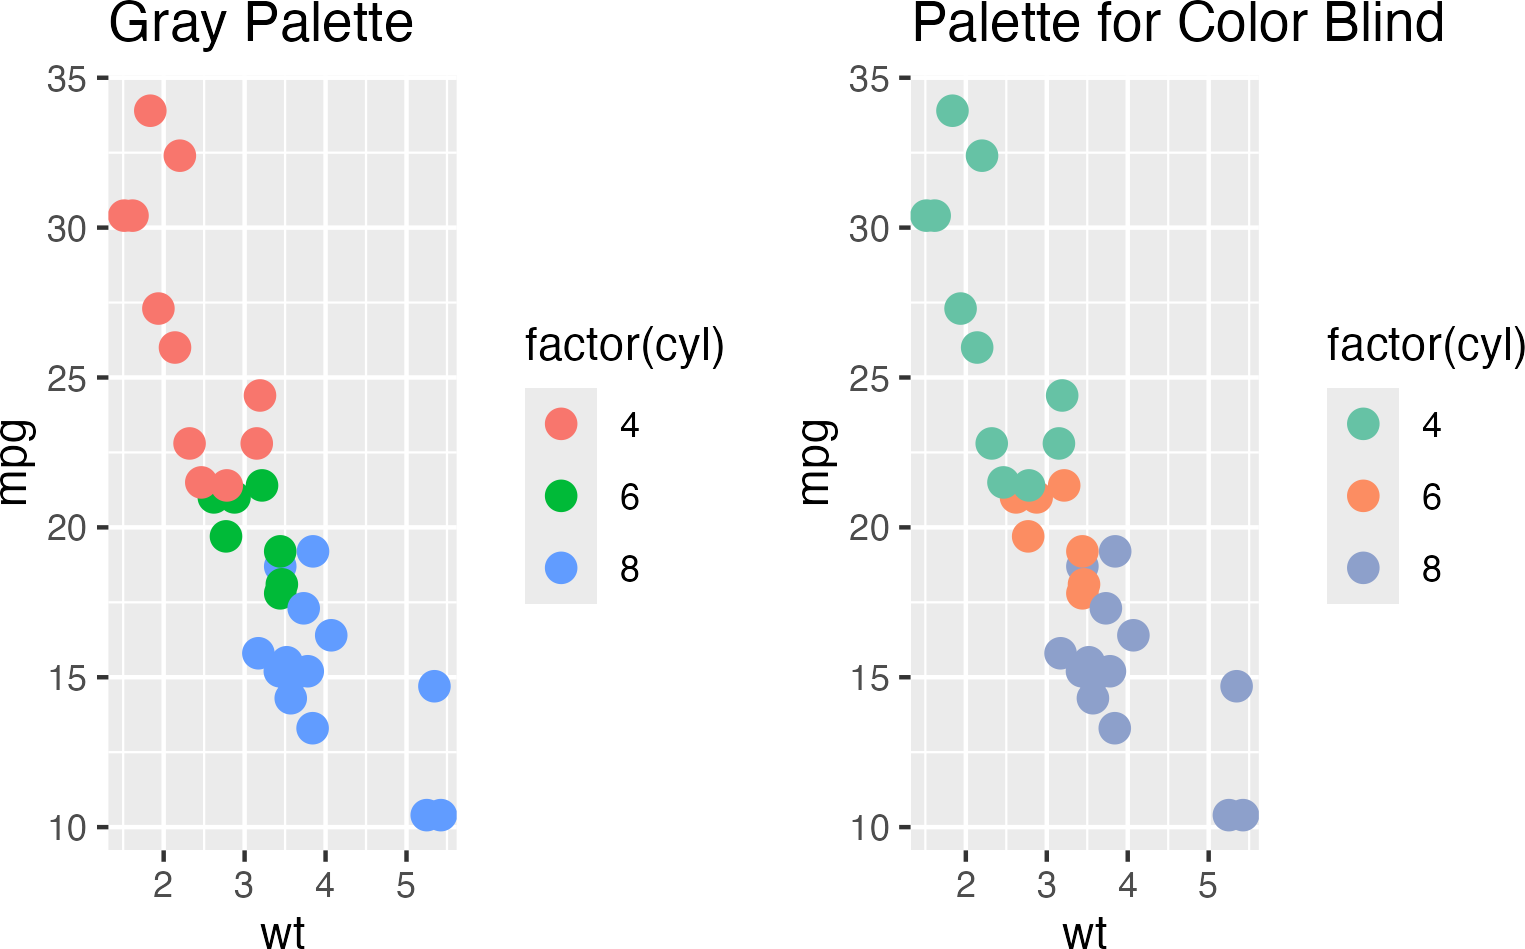
\includegraphics{chapter04_files/figure-pdf/unnamed-chunk-2-1.png}

また,\texttt{ggplot2}のデフォルト設定では,背景色が灰色になっている。これは全体のテーマとして\texttt{theme\_gray()}が設定されているからである。しかし日本心理学会の\href{https://psych.or.jp/manual/}{執筆・投稿の手引き}に記載されているグラフの例を見ると,背景は白色とされている。このような設定に変更するためには,theme\_classic()やtheme\_bw()を用いる。

\begin{Shaded}
\begin{Highlighting}[]
\NormalTok{p2 }\SpecialCharTok{+} \FunctionTok{theme\_classic}\NormalTok{()}
\end{Highlighting}
\end{Shaded}

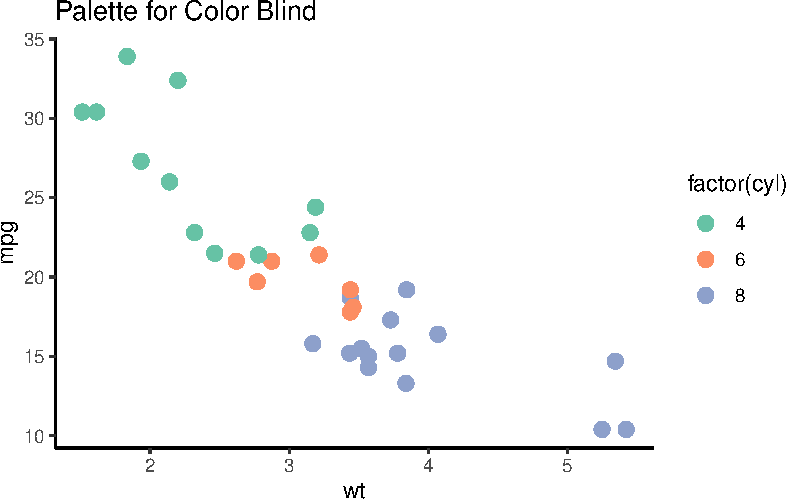
\includegraphics{chapter04_files/figure-pdf/unnamed-chunk-3-1.pdf}

このほかにも,様々な描画上の工夫は考えられる。目標となる図版のレシピを書き起こせるように,要素に分解ができれば,殆どのケースにおいて問題を解決することができるだろう。

\section{マークダウンと描画の課題}\label{ux30deux30fcux30afux30c0ux30a6ux30f3ux3068ux63cfux753bux306eux8ab2ux984c}

\begin{itemize}
\tightlist
\item
  今日の課題はRmarkdownで記述してください。著者名に学籍番号と名前を含め,適宜見出しをつくり,かつ,平文で以下に挙げる課題を記載することでどの課題に対する回答のコード(チャンク)であるかわかるようにしてください。
\end{itemize}

\begin{enumerate}
\def\labelenumi{\arabic{enumi}.}
\tightlist
\item
  \texttt{Baseball.csv}
  を読み込み,2020年度のデータセットに限定し,以下の操作に必要であれば変数の変換をすませたデータセット,\texttt{dat.tb}を用意してください。
\item
  \texttt{dat.tb}の身長変数を使って、ヒストグラムを描いてください。この時,テーマを\texttt{theme\_classic}にしてください。。
\item
  \texttt{dat.tb}の身長変数と体重変数を使って、散布図を描いてください。この時,テーマを\texttt{theme\_bw}にしてください。
\item
  (承前)
  散布図の各点を血液型で塗り分けてください。この時,カラーパレットを\texttt{Set3}に変えてください。
\item
  (承前) 散布図の点の形を血液型で変えてください。
\item
  \texttt{dat.tb}の身長と体重についての散布図を、チームごとに分割してください。
\item
  (承前)
  \texttt{geom\_smooth()}でスムーズな線を引いてください。特に\texttt{method}を指定する必要はありません。
\item
  (承前)
  \texttt{geom\_smooth()}で直線関数を引いてください。\texttt{method="lm"}
  と指定するといいでしょう。
\item
  x軸は身長、y軸は体重の平均値をプロットしてください。方法はいろいろありますが,要約統計量を計算した別のデータセット\texttt{dat.tb2}を作るか,幾何学オブジェクトの中で,次のように関数を適用することもできます。ヒント:\texttt{geom\_point(stat="summary",\ fun=mean)}。
\item
  課題2,4および体重のヒストグラムをつかって下の図を描き,\texttt{ggsave}関数を使って保存するコードを書いてください。ファイル名やその他オプションは任意です。
\end{enumerate}

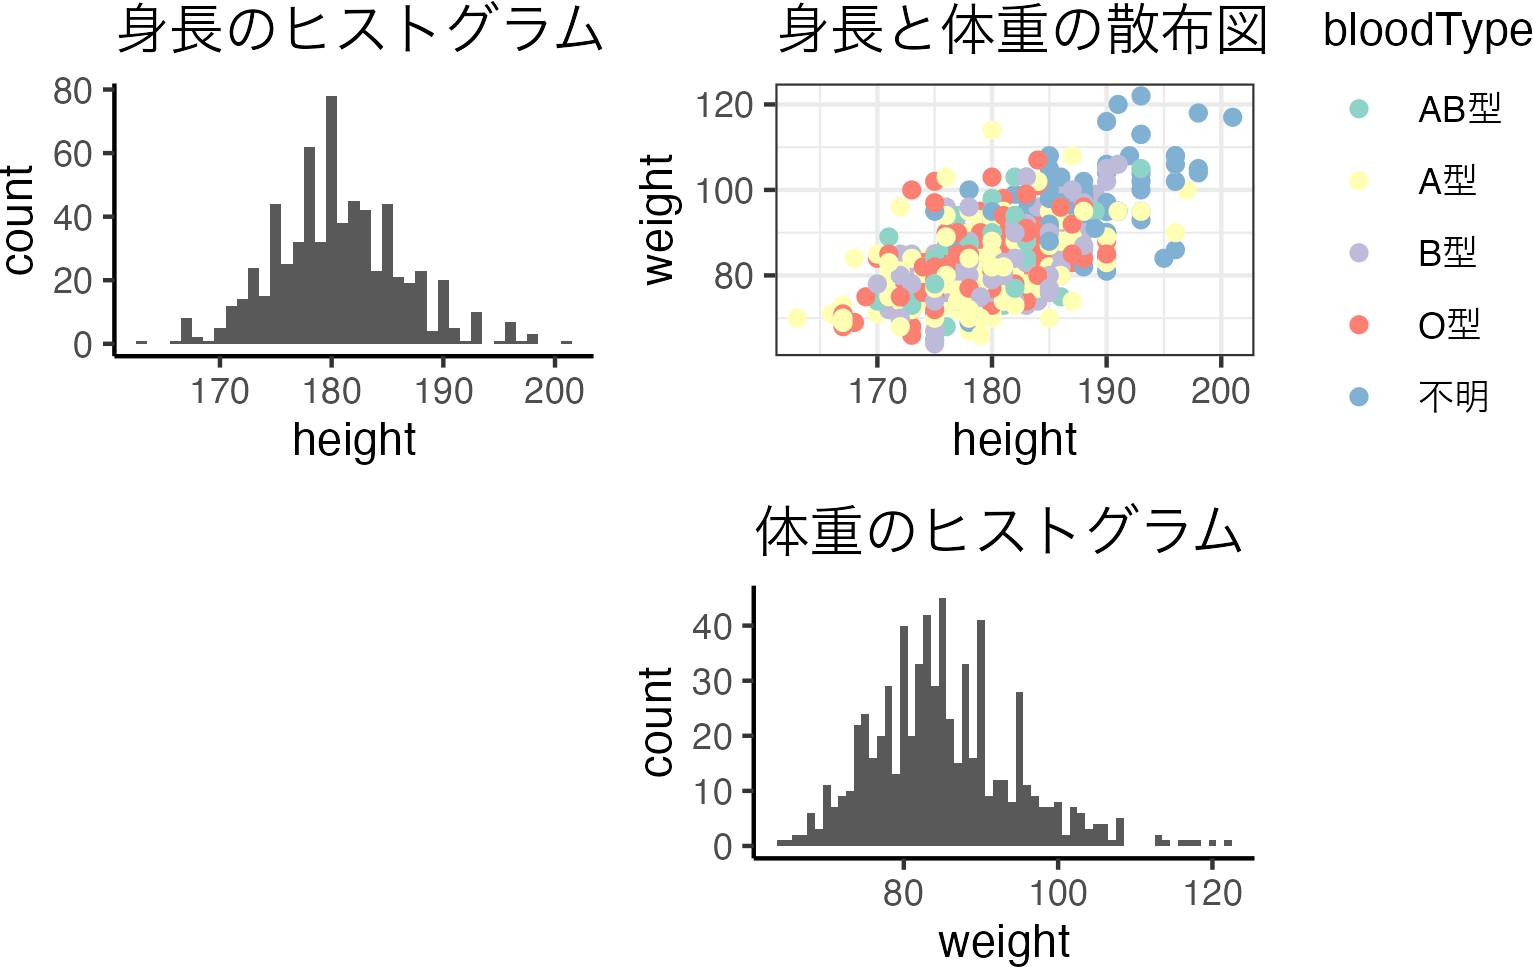
\includegraphics{chapter04_files/figure-pdf/unnamed-chunk-4-1.png}

\bookmarksetup{startatroot}

\chapter{Rでプログラミング}\label{rux3067ux30d7ux30edux30b0ux30e9ux30dfux30f3ux30b0}

ここではプログラミング言語としてのRについて解説する。 なお副読本として
\textcite{kosugi2023}
を挙げておく。また,プログラミングのより専門的な理解のために,\textcite{Jared_P_Lander2018-12-28},
\textcite{Ren_Kun2017-11-23}, \textcite{Hadley_Wickham2016-02-10}
なども参考にすると良い。

プログラミング言語は,古くはCやJava,最近ではPythonやJuliaなどがよく用いられている。Rも統計パッケージというよりプログラミング言語として考えるのが適切かもしれない。Rは他のプログラミング言語に比べて,変数の型宣言を事前にしなくても良いことや,インデントなど書式についておおらかなところは,初心者にとって使いやすいところだろう。一方で,ベクトルの再利用のところで注意したように(Section~\ref{sec-vector}),不足分を補うために先回りして補填されたり,この後解説する関数の作成時に明示的な指定がなければ環境変数を参照する点など,親切心が空回りするところがある。より厳格な他言語になれていると,こうした点はかえって不便に思えるところもあるかもしれない。総じて,R言語は初心者向けであるといえるだろう。

さて,世にプログラミング言語は多くあれど\footnote{\textcite{Language2016}
  には117種もの計算機言語が紹介されている。},その全てに精通する必要はないし,不可能である。それよりも,プログラミング言語一般に通底する基本的概念を知り,あとは各言語による「方言」がある,と考えた方が生産的である。その基本的概念を3つ挙げるとすれば,「代入」「反復」「条件分岐」になるだろう。

\section{代入}\label{ux4ee3ux5165}

代入は,言い換えればオブジェクト(メモリ)に保管することを指す。これについては既に
Chapter~\ref{sec-Rbase}
で触れた通りであり,ここでは言及しない。オブジェクトや変数の型,常に上書きされる性質に注意しておけば十分だろう。

一点だけ追加で説明しておくと,次のような表現がなされることがある。

\begin{Shaded}
\begin{Highlighting}[]
\NormalTok{a }\OtherTok{\textless{}{-}} \DecValTok{0}
\NormalTok{a }\OtherTok{\textless{}{-}}\NormalTok{ a }\SpecialCharTok{+} \DecValTok{1}
\FunctionTok{print}\NormalTok{(a)}
\end{Highlighting}
\end{Shaded}

\begin{verbatim}
[1] 1
\end{verbatim}

ここではあえて,代入記号として\texttt{=}を使った。2行目に\texttt{a\ =\ a\ +\ 1}
とあるが,これを見て数式のように解釈しようとすると混乱する。数学的には明らかにおかしな表現だが,これは上書きと代入というプログラミング言語の特徴を使ったもので,「(いま保持している)\texttt{a}の値に1を加えたものを,(新しく同じ名前のオブジェクト)\texttt{a}に代入する(=上書きする)」という意味である。この方法で,\texttt{a}
をカウンタ変数として用いることがある。誤読の可能性を下げるため,この授業においては代入記号を\texttt{\textless{}-}としている。

このオブジェクトを上書きするという特徴は多くの言語に共通したものであり,間違いを避けるためには,オブジェクトを作る時に初期値を設定することが望ましい。先の例では,代入の直上で\texttt{a\ \textless{}-\ 0}としており,オブジェクト\texttt{a}
に\texttt{0}
を初期値として与えている。この変数の初期化作業がないと,以前に使っていた値を引き継いでしまう可能性があるので,今から新しく使う変数を作りたいというときは,このように明示しておくといいだろう。

なお,変数をメモリから明示的に削除する場合は,\texttt{remove}関数を使う。

\begin{Shaded}
\begin{Highlighting}[]
\FunctionTok{remove}\NormalTok{(a)}
\end{Highlighting}
\end{Shaded}

これを実行すると,RStudioのEnvironmentタブからオブジェクト\texttt{a}が消えたことがわかるだろう。
メモリの一斉除去は,同じくRStudioのEnvironmentタブにある箒マークをクリックするか,\texttt{remove(list=ls())}とすると良い\footnote{\texttt{ls()}関数はlist
  objectsの意味で,メモリにあるオブジェクトのリストを作る関数}。

\section{反復}\label{ux53cdux5fa9}

\subsection{for文}\label{forux6587}

電子計算機の特徴は,電源等のハードウェア的問題がなければ疲労することなく計算を続けられるところにある。人間は反復によって疲労が溜まったり,集中力が欠如するなどして単純ミスを生成するが,電子計算機にそういったところはない。

このように反復計算は電子計算機の中心的特徴であり,細々した計算作業を指示した期間反復させ続けることができる。反復の代表的なコマンドは\texttt{for}であり,forループなどと呼ばれる。forループはプログラミングの基本的な制御構造であり,R言語の\texttt{for}ループの基本的な構文は次のようになる:

\begin{Shaded}
\begin{Highlighting}[]
\ControlFlowTok{for}\NormalTok{ (value }\ControlFlowTok{in}\NormalTok{ sequence) \{}
    \CommentTok{\# 実行するコード}
\NormalTok{\}}
\end{Highlighting}
\end{Shaded}

ここの\texttt{value}は各反復で\texttt{sequence}の次の要素を取る反復インデックス変数である。。\texttt{sequence}は一般にベクトルやリストなどの配列型のデータであり,「\#実行するコード」はループ体内で実行される一連の命令になる。

以下は\texttt{for}文の例である。

\begin{Shaded}
\begin{Highlighting}[]
\ControlFlowTok{for}\NormalTok{ (i }\ControlFlowTok{in} \DecValTok{1}\SpecialCharTok{:}\DecValTok{5}\NormalTok{) \{}
  \FunctionTok{cat}\NormalTok{(}\StringTok{"現在の値は"}\NormalTok{, i, }\StringTok{"です。}\SpecialCharTok{\textbackslash{}n}\StringTok{"}\NormalTok{)}
\NormalTok{\}}
\end{Highlighting}
\end{Shaded}

\begin{verbatim}
現在の値は 1 です。
現在の値は 2 です。
現在の値は 3 です。
現在の値は 4 です。
現在の値は 5 です。
\end{verbatim}

\texttt{for}
文は続く小括弧のなかである変数を宣言し(ここでは\texttt{i}),それがどのように変化するか(ここでは\texttt{1:5},すなわち1,2,3,4,5)を指定する。続く中括弧の中で,反復したい操作を記入する。今回は\texttt{cat}
文によるコンソールへの文字力の出力を行っている。ここでのコマンドは複数あってもよく,中括弧が閉じられるまで各行のコマンドが実行される。

次に示すは,\texttt{sequence}にあるベクトルが指定されているので,反復インデックス変数が連続的に変化しない例である。

\begin{Shaded}
\begin{Highlighting}[]
\ControlFlowTok{for}\NormalTok{ (i }\ControlFlowTok{in} \FunctionTok{c}\NormalTok{(}\DecValTok{2}\NormalTok{, }\DecValTok{4}\NormalTok{, }\DecValTok{12}\NormalTok{, }\DecValTok{3}\NormalTok{, }\SpecialCharTok{{-}}\DecValTok{6}\NormalTok{)) \{}
  \FunctionTok{cat}\NormalTok{(}\StringTok{"現在の値は"}\NormalTok{, i, }\StringTok{"です。}\SpecialCharTok{\textbackslash{}n}\StringTok{"}\NormalTok{)}
\NormalTok{\}}
\end{Highlighting}
\end{Shaded}

\begin{verbatim}
現在の値は 2 です。
現在の値は 4 です。
現在の値は 12 です。
現在の値は 3 です。
現在の値は -6 です。
\end{verbatim}

また,反復はネスト(入れ子)になることもできる。次の例を見てみよう。

\begin{Shaded}
\begin{Highlighting}[]
\CommentTok{\# 2次元の行列を定義}
\NormalTok{A }\OtherTok{\textless{}{-}} \FunctionTok{matrix}\NormalTok{(}\DecValTok{1}\SpecialCharTok{:}\DecValTok{9}\NormalTok{, }\AttributeTok{nrow =} \DecValTok{3}\NormalTok{)}

\CommentTok{\# 行ごとにループ}
\ControlFlowTok{for}\NormalTok{ (i }\ControlFlowTok{in} \DecValTok{1}\SpecialCharTok{:}\FunctionTok{nrow}\NormalTok{(A)) \{}
  \CommentTok{\# 列ごとにループ}
  \ControlFlowTok{for}\NormalTok{ (j }\ControlFlowTok{in} \DecValTok{1}\SpecialCharTok{:}\FunctionTok{ncol}\NormalTok{(A)) \{}
    \FunctionTok{cat}\NormalTok{(}\StringTok{"要素 ["}\NormalTok{, i, }\StringTok{", "}\NormalTok{, j, }\StringTok{"]は "}\NormalTok{, A[i, j], }\StringTok{"}\SpecialCharTok{\textbackslash{}n}\StringTok{"}\NormalTok{)}
\NormalTok{  \}}
\NormalTok{\}}
\end{Highlighting}
\end{Shaded}

\begin{verbatim}
要素 [ 1 ,  1 ]は  1 
要素 [ 1 ,  2 ]は  4 
要素 [ 1 ,  3 ]は  7 
要素 [ 2 ,  1 ]は  2 
要素 [ 2 ,  2 ]は  5 
要素 [ 2 ,  3 ]は  8 
要素 [ 3 ,  1 ]は  3 
要素 [ 3 ,  2 ]は  6 
要素 [ 3 ,  3 ]は  9 
\end{verbatim}

ここで,反復インデックス変数が\texttt{i}と\texttt{j}というように異なる名称になっていることに注意しよう。例えば今回,ここで両者を\texttt{i}にしてしまうと,行変数なのか列変数なのかわからなくなってしまう。また少し専門的になるが,R言語は\texttt{for}文で宣言されるたびに,内部で反復インデックス変数を新しく生成している(異なるメモリを割り当てる)ためにエラーにならないが,他言語の場合は同じ名前のオブジェクトと判断されることが一般的であり,その際は値が終了値に到達せず計算が終わらないといったバグを引き起こす。反復に使う汎用的な変数名として\texttt{i,j,k}がよく用いられるため,自身のスクリプトの中でオブジェクト名として単純な一文字にすることは避けた方がいいだろう。

\subsection{while文}\label{whileux6587}

whileループはプログラミングの基本構造であり,特定の条件が真(True)である間,繰り返し一連の命令を実行する。「``while''(~する間)」という名前から直感的に理解できるだろう。

R言語のwhileループの基本的な構文は次のようになる:

\begin{Shaded}
\begin{Highlighting}[]
\ControlFlowTok{while}\NormalTok{ (condition) \{}
    \CommentTok{\# 実行するコード}
\NormalTok{\}}
\end{Highlighting}
\end{Shaded}

ここで,「condition」はループが終了するための条件である。「\#
実行するコード」はループ体内で実行される一連の指示である。たとえば,1から10までの値を出力する\texttt{while}ループは以下のように書くことができる:

\begin{Shaded}
\begin{Highlighting}[]
\NormalTok{i }\OtherTok{\textless{}{-}} \DecValTok{1}
\ControlFlowTok{while}\NormalTok{ (i }\SpecialCharTok{\textless{}=} \DecValTok{5}\NormalTok{) \{}
  \FunctionTok{print}\NormalTok{(i)}
\NormalTok{  i }\OtherTok{\textless{}{-}}\NormalTok{ i }\SpecialCharTok{+} \DecValTok{1}
\NormalTok{\}}
\end{Highlighting}
\end{Shaded}

\begin{verbatim}
[1] 1
[1] 2
[1] 3
[1] 4
[1] 5
\end{verbatim}

このコードでは,「i」が5以下である限りループが続く。「print(i)」で「i」の値が表示され,「i
\textless- i +
1」で「i」の値が1ずつ増加する。これにより,「i」の値が10を超えると条件が偽(False)となり,ループが終了する。

whileループを使用する際の一般的な注意点は,無限ループ(終わらないループ)を避けることである。これは,conditionが常に真(True)である場合に発生する。そのような状況を避けるためには,ループ内部で何らかの形でconditionが最終的に偽(False)となるようにコードを記述することが必要である。

また,R言語は他の多くのプログラミング言語と異なり,ベクトル化された計算を効率的に行う設計がされている。したがって,可能な限り\texttt{for}ループや\texttt{while}ループを使わずに,ベクトル化した表現を利用すれば計算速度を上げることができる。

\section{条件分岐}\label{ux6761ux4ef6ux5206ux5c90}

条件分岐はプログラム内で特定の条件を指定し,その条件が満たされるかどうかによって異なる処理を行うための制御構造である。R言語では
\texttt{if-else} を用いて条件分岐を表現する。

\subsection{\texorpdfstring{\texttt{if}
文の基本的な構文}{if 文の基本的な構文}}\label{if-ux6587ux306eux57faux672cux7684ux306aux69cbux6587}

以下が \texttt{if} 文の基本的な構文になる:

\begin{Shaded}
\begin{Highlighting}[]
\ControlFlowTok{if}\NormalTok{ (条件) \{}
    \CommentTok{\# 条件が真である場合に実行するコード}
\NormalTok{\}}
\end{Highlighting}
\end{Shaded}

\texttt{if}
の後の小括弧内に条件を指定する。この条件が真(TRU)であれば,その後の
中括弧\texttt{\{\}} 内のコードが実行される。さらに,\texttt{else}
を使用して,条件が偽(FALSE)の場合の処理を追加することもできる:

\begin{Shaded}
\begin{Highlighting}[]
\ControlFlowTok{if}\NormalTok{ (条件) \{}
    \CommentTok{\# 条件が真である場合に実行するコード}
\NormalTok{\} }\ControlFlowTok{else}\NormalTok{ \{}
    \CommentTok{\# 条件が偽である場合に実行するコード}
\NormalTok{\}}
\end{Highlighting}
\end{Shaded}

以下に具体的な使用例を示そう:

\begin{Shaded}
\begin{Highlighting}[]
\NormalTok{x }\OtherTok{\textless{}{-}} \DecValTok{10}

\ControlFlowTok{if}\NormalTok{ (x }\SpecialCharTok{\textgreater{}} \DecValTok{0}\NormalTok{) \{}
  \FunctionTok{print}\NormalTok{(}\StringTok{"x is positive"}\NormalTok{)}
\NormalTok{\} }\ControlFlowTok{else}\NormalTok{ \{}
  \FunctionTok{print}\NormalTok{(}\StringTok{"x is not positive"}\NormalTok{)}
\NormalTok{\}}
\end{Highlighting}
\end{Shaded}

\begin{verbatim}
[1] "x is positive"
\end{verbatim}

このコードでは,変数 \texttt{x}
が正の場合とそうでない場合で異なるメッセージを出力する。

条件は論理式(例:\texttt{x\ \textgreater{}\ 0},
\texttt{y\ ==\ 1})や論理値(TRUE/FALSE)を返す関数・操作(例:\texttt{is.numeric(x)})などで指定する。また,複数の条件を組み合わせる際には論理演算子(\texttt{\&\&},
\texttt{\textbar{}\textbar{}})を使用する。

この例では,\texttt{x}が正と\texttt{y}が負の場合に特定のメッセージを出力する。それ以外の場合は,「Other
case」と出力される。\texttt{x}や\texttt{y}の値を色々変えて,試してみて欲しい。

\begin{Shaded}
\begin{Highlighting}[]
\NormalTok{x }\OtherTok{\textless{}{-}} \DecValTok{10}
\NormalTok{y }\OtherTok{\textless{}{-}} \SpecialCharTok{{-}}\DecValTok{3}

\ControlFlowTok{if}\NormalTok{ (x }\SpecialCharTok{\textgreater{}} \DecValTok{0} \SpecialCharTok{\&\&}\NormalTok{ y }\SpecialCharTok{\textless{}} \DecValTok{0}\NormalTok{) \{}
  \FunctionTok{print}\NormalTok{(}\StringTok{"x is positive and y is negative"}\NormalTok{)}
\NormalTok{\} }\ControlFlowTok{else}\NormalTok{ \{}
  \FunctionTok{print}\NormalTok{(}\StringTok{"Other case"}\NormalTok{)}
\NormalTok{\}}
\end{Highlighting}
\end{Shaded}

\begin{verbatim}
[1] "x is positive and y is negative"
\end{verbatim}

\section{反復と条件分岐に関する練習問題}\label{ux53cdux5fa9ux3068ux6761ux4ef6ux5206ux5c90ux306bux95a2ux3059ux308bux7df4ux7fd2ux554fux984c}

\begin{enumerate}
\def\labelenumi{\arabic{enumi}.}
\tightlist
\item
  1から20までの数字で,偶数だけをプリントするプログラムを書いてください。
\item
  1から40までの数値をプリントするプログラムを書いてください。ただしその数値に3がつく(1か10の位の値が3である)か,3の倍数の時だけ,数字の後ろに「サァン!」という文字列をつけて出力してください。
\item
  ベクトル \texttt{c(1,\ -2,\ 3,\ -4,\ 5)} の各要素について,正なら
  ``positive'',負なら ``negative''
  をプリントするプログラムを書いてください。
\item
  次の行列\(A\)と\(B\)の掛け算を計算するプログラムを書いてください。なお,Rで行列の積は\texttt{\%*\%}という演算子を使いますが,ここでは\texttt{for}文を使ったプログラムにしてください。出来上がる行列の\(i\)行\(j\)列目の要素\(c_{ij}\)は,行列\(A\)の第\(i\)行の各要素と,行列\(B\)の第\(j\)列目の各要素の積和,すなわち\[c_{ij}=\sum_{k} a_{ik}b_{kj}\]になります。検算用のコードを下に示します。
\end{enumerate}

\begin{Shaded}
\begin{Highlighting}[]
\NormalTok{A }\OtherTok{\textless{}{-}} \FunctionTok{matrix}\NormalTok{(}\DecValTok{1}\SpecialCharTok{:}\DecValTok{6}\NormalTok{, }\AttributeTok{nrow =} \DecValTok{3}\NormalTok{)}
\NormalTok{B }\OtherTok{\textless{}{-}} \FunctionTok{matrix}\NormalTok{(}\DecValTok{3}\SpecialCharTok{:}\DecValTok{10}\NormalTok{, }\AttributeTok{nrow =} \DecValTok{2}\NormalTok{)}
\DocumentationTok{\#\# 課題になる行列}
\FunctionTok{print}\NormalTok{(A)}
\end{Highlighting}
\end{Shaded}

\begin{verbatim}
     [,1] [,2]
[1,]    1    4
[2,]    2    5
[3,]    3    6
\end{verbatim}

\begin{Shaded}
\begin{Highlighting}[]
\FunctionTok{print}\NormalTok{(B)}
\end{Highlighting}
\end{Shaded}

\begin{verbatim}
     [,1] [,2] [,3] [,4]
[1,]    3    5    7    9
[2,]    4    6    8   10
\end{verbatim}

\begin{Shaded}
\begin{Highlighting}[]
\DocumentationTok{\#\# 求めるべき答え}
\NormalTok{C }\OtherTok{\textless{}{-}}\NormalTok{ A }\SpecialCharTok{\%*\%}\NormalTok{ B}
\FunctionTok{print}\NormalTok{(C)}
\end{Highlighting}
\end{Shaded}

\begin{verbatim}
     [,1] [,2] [,3] [,4]
[1,]   19   29   39   49
[2,]   26   40   54   68
[3,]   33   51   69   87
\end{verbatim}

\section{関数を作る}\label{ux95a2ux6570ux3092ux4f5cux308b}

複雑なプログラムも,ここまでの代入、反復,条件分岐の組み合わせからなる。回帰分析や因子分析のような統計モデルを実行するときに,統計パッケージのユーザとしては,統計モデルを実現してくれる関数にデータを与えて答えを受け取るだけであるが,そのアルゴリズムはこれらプログラミングのピースを紡いでつくられているのである。

ここでは関数を自分で作ることを考える。といっても身構える必要はない。表計算ソフトウェアで同じような操作を繰り返すときにマクロに記録するように,R上で同じようなコードを何度も書く機会があるならば,それを関数という名のパッケージにしておこう,ということである。関数化しておくことで手続きをまとめることができ,小単位に分割できるため並列して開発したり,バグを見つけやすくなるという利点がある。

\subsection{基本的な関数の作り方}\label{ux57faux672cux7684ux306aux95a2ux6570ux306eux4f5cux308aux65b9}

関数が受け取る値のことを\textbf{引数}(ひきすう,argment)といい,また関数が返す値のことを\textbf{戻り値}(もどりち,value)という。\(y=f(x)\)という式は,引数が\texttt{x}で戻り値が\texttt{y}な関数\(f\),と言い換えることができるだろう。

Rの関数を書く基本的な構文は以下のようになる。

\begin{Shaded}
\begin{Highlighting}[]
\NormalTok{function\_name }\OtherTok{\textless{}{-}} \ControlFlowTok{function}\NormalTok{(argument) \{}
   \CommentTok{\# function body}
   \FunctionTok{return}\NormalTok{(value)}
\NormalTok{\}}
\end{Highlighting}
\end{Shaded}

ここで\texttt{function\ body}とあるのは計算本体である。例えば与えられた数字に\texttt{3}を足して返す関数,\texttt{add3}を作ってみよう。プログラムは以下のようになる。

\begin{Shaded}
\begin{Highlighting}[]
\NormalTok{add3 }\OtherTok{\textless{}{-}} \ControlFlowTok{function}\NormalTok{(x) \{}
\NormalTok{  x }\OtherTok{\textless{}{-}}\NormalTok{ x }\SpecialCharTok{+} \DecValTok{3}
  \FunctionTok{return}\NormalTok{(x)}
\NormalTok{\}}
\CommentTok{\# 実行例}
\FunctionTok{add3}\NormalTok{(}\DecValTok{5}\NormalTok{)}
\end{Highlighting}
\end{Shaded}

\begin{verbatim}
[1] 8
\end{verbatim}

また,2つの値を足し合わせる関数は次のようになる。

\begin{Shaded}
\begin{Highlighting}[]
\NormalTok{add\_numbers }\OtherTok{\textless{}{-}} \ControlFlowTok{function}\NormalTok{(a, b) \{}
\NormalTok{  sum }\OtherTok{\textless{}{-}}\NormalTok{ a }\SpecialCharTok{+}\NormalTok{ b}
  \FunctionTok{return}\NormalTok{(sum)}
\NormalTok{\}}
\CommentTok{\# 実行例}
\FunctionTok{add\_numbers}\NormalTok{(}\DecValTok{2}\NormalTok{, }\DecValTok{5}\NormalTok{)}
\end{Highlighting}
\end{Shaded}

\begin{verbatim}
[1] 7
\end{verbatim}

ここで示したように,引数は複数取ることも可能である。また,既定値default
valueを設定することも可能である。次の例を見てみよう。

\begin{Shaded}
\begin{Highlighting}[]
\NormalTok{add\_numbers2 }\OtherTok{\textless{}{-}} \ControlFlowTok{function}\NormalTok{(a, }\AttributeTok{b =} \DecValTok{1}\NormalTok{) \{}
\NormalTok{  sum }\OtherTok{\textless{}{-}}\NormalTok{ a }\SpecialCharTok{+}\NormalTok{ b}
  \FunctionTok{return}\NormalTok{(sum)}
\NormalTok{\}}
\CommentTok{\# 実行例}
\FunctionTok{add\_numbers2}\NormalTok{(}\DecValTok{2}\NormalTok{, }\DecValTok{5}\NormalTok{)}
\end{Highlighting}
\end{Shaded}

\begin{verbatim}
[1] 7
\end{verbatim}

\begin{Shaded}
\begin{Highlighting}[]
\FunctionTok{add\_numbers2}\NormalTok{(}\DecValTok{4}\NormalTok{)}
\end{Highlighting}
\end{Shaded}

\begin{verbatim}
[1] 5
\end{verbatim}

関数を作るときに,\texttt{(a,b=1)}としているのは,\texttt{b}に既定値として\texttt{1}を与えていて,特に指定がなければこの値を使うよう指示しているということである。実行例において,引数が2つ与えられている場合はそれらを使った計算をし(\texttt{2+5}),1つしか与えられていない場合は第一引数\texttt{a}に与えられた値を,第二引数\texttt{b}は既定値を使った計算をする(\texttt{4+1}),という挙動になる。

ここから推察できるように,われわれユーザが使う統計パッケージの関数にも実は多くの引数があり,既定値が与えられているということだ。これらは選択的に,あるいは能動的に与えることができるものであるが,これらの引数は選択的に指定することができるのだが,通常は一般的に使われる値や計算の細かな設定に関するものであり,開発者がユーザの手間を省くために提供しているものである。関数のヘルプを見ると指定可能な引数の一覧が表示されるので,ぜひ興味を持って見てもらいたい。

\subsection{複数の戻り値}\label{ux8907ux6570ux306eux623bux308aux5024}

Rでの戻り値は1つのオブジェクトでなければならない。しかし,複数の値を返したいということがあるだろう。そのような場合は,返すオブジェクトを\texttt{list}などでひとまとめにして作成すると良い。以下に簡単な例を示す。

\begin{Shaded}
\begin{Highlighting}[]
\NormalTok{calculate\_values }\OtherTok{\textless{}{-}} \ControlFlowTok{function}\NormalTok{(a, b) \{}
\NormalTok{  sum }\OtherTok{\textless{}{-}}\NormalTok{ a }\SpecialCharTok{+}\NormalTok{ b}
\NormalTok{  diff }\OtherTok{\textless{}{-}}\NormalTok{ a }\SpecialCharTok{{-}}\NormalTok{ b}
  \CommentTok{\# 戻り値として名前付きリストを作成}
\NormalTok{  result }\OtherTok{\textless{}{-}} \FunctionTok{list}\NormalTok{(}\StringTok{"sum"} \OtherTok{=}\NormalTok{ sum, }\StringTok{"diff"} \OtherTok{=}\NormalTok{ diff)}
  \FunctionTok{return}\NormalTok{(result)}
\NormalTok{\}}
\CommentTok{\# 実行例}
\NormalTok{result }\OtherTok{\textless{}{-}} \FunctionTok{calculate\_values}\NormalTok{(}\DecValTok{10}\NormalTok{, }\DecValTok{5}\NormalTok{)}
\CommentTok{\# 結果を表示}
\FunctionTok{print}\NormalTok{(result)}
\end{Highlighting}
\end{Shaded}

\begin{verbatim}
$sum
[1] 15

$diff
[1] 5
\end{verbatim}

\section{関数化の練習問題}\label{ux95a2ux6570ux5316ux306eux7df4ux7fd2ux554fux984c}

\begin{enumerate}
\def\labelenumi{\arabic{enumi}.}
\tightlist
\item
  ある値を与えたとき,正の値なら''positive'',負の値なら''negative'',0のときは''Zero''と表示する関数を書いてください。
\item
  ある2組の数字を与えた時,和,差,積,商を返す関数を書いてください。
\item
  あるベクトルを与えた時,算術平均,中央値,最大値,最小値,範囲を返す関数を書いてください。
\item
  あるベクトルを与えた時,標本分散を返す関数を書いてください。なおRの分散を返す関数\texttt{var}は不偏分散\(\hat{\sigma}\)を返しており,標本分散\texttt{v}とは計算式が異なります。念のため,計算式を以下に示します。
  \[\hat{\sigma} = \frac{1}{n-1}\sum_{i=1}^n (x_i - \bar{x})^2 \]
  \[v= \frac{1}{n}\sum_{i=1}^n (x_i - \bar{x})^2 \]
\end{enumerate}

\bookmarksetup{startatroot}

\chapter{確率とシミュレーション}\label{ux78baux7387ux3068ux30b7ux30dfux30e5ux30ecux30fcux30b7ux30e7ux30f3}

\section{確率の考え方と使い所}\label{ux78baux7387ux306eux8003ux3048ux65b9ux3068ux4f7fux3044ux6240}

統計と確率は密接な関係がある。
まずデータをたくさん集めると,個々のケースでは見られない全体的な傾向が見られるようになり,それを表現するのに確率の考え方を使う,というのがひとつ。
次にデータがそれほどたくさんなくとも,大きな全体の中から一部を取り出した標本Sampleと考えられるとき,標本は全体の性質をどのように反映しているかを考えることになる。ここで全体の傾向から一部を取り出した偶然性を表現するときに確率の考え方を使うことになる。
最後に,理論的・原理的に挙動がわかっている機械のようなものでも,現実的・実践的には系統だったズレが生じたり,偶然としか考えられない誤差が紛れ込むことがある。前者は機械の調整で対応できるが,後者は偶然が従う確率を考える必要がある。

心理学は人間を対象に研究を行うが,あらゆる人間を一度に調べるわけにはいかないので,サンプルを取り出して調査したり実験したりする(第2のケース)。データサイエンスでは何万レコードというおおきなデータセットになるが,心理学の場合は数件から数十件しかないことも多い。また,心理学的傾向を理論立ててモデル化できたとしても,実際の行動には誤差が含まれている可能性が高い(第3のケース)。このことから,心理学で得られるデータは確率変数として考えられ,小標本から母集団の性質を推測する\textbf{推測統計}と共に利用される。

厳密に数学的な意味での\textbf{確率}は,集合,積分,測度といった緻密な概念の積み重ねから定義される\footnote{詳しくは
  \textcite{Yoshida2021-02-25} , \textcite{Kono1999-05-01},
  \textcite{Sato1994-02-25} などを参照のこと。}。ここではその詳細に分け入らず,単に「特定の結果が生じる可能性について,0から1の間の実数でその大小を表現したもの」とだけ理解しておいて欲しい。この定義からは,「全ての可能な組み合わせのうち当該事象の成立する割合」という解釈も成り立つし,「主観的に重みづけた真実味の強さに関する信念の度合い」という解釈も成り立つ。\footnote{前者の解釈は高校までの数学で学ぶ確率であり,頻度主義的確率と呼ばれることがある。一方後者の解釈は,降水確率X\%のように日常でも使うものであり,主観確率と呼ばれることがある。こうした解釈の違いを,主義主張の対立であって数学的ではない,と批判する向きもあるが,実際コルモゴロフの公理はどちらの立場でも成立するように整えられており,筆者個人的にはユーザが理解しやすく計算できればどちらでも良いと考えている。}
これまで学んできた確率は順列・組み合わせを全て書き出す退屈なもの,と思っていたかもしれないが,「十中八九まちがいないね(80-90\%ほど確からしいと考えている)」という数字も確率の一種として扱えるので,非常に身近で適用範囲の広い概念である。理解を進めるポイントの1つとして,確率を面積として考えると良いかもしれない。ありうる状況の全体の空間に対して,事象の成立する程度がどの程度の面積がどの程度の割合であるかを表現したのが確率という量である,と考えるのである(
\textcite{Hiraoka200910}
は書籍の中で一貫して面積で説明している。この説明だと,条件付き確率などの理解がしやすい。)。

ただし注意して区別しておいて欲しいのが,確率変数とその実現値の違いである。データセットやスプレッドシートに含まれる値は,あくまでも\textbf{確率変数の実現値}というのであって,\textbf{確率変数}はその不確実な状態を有した変数そのものを指す言葉である。サイコロは確率変数だが,サイコロの出目は確率変数の実現値である。心理変数は確率変数だが,手に入れたデータはその実現値である。実現値を通じて変数の特徴を知り,全体を推測するという流れである。

目の前のデータを超えて,抽象的な実体で議論を進めることが難しく感じられるかもしれない。実は誰しもそうなのであって,確率の正確な理解は非常に難易度が高い。しかしRなど計算機言語に実装されている関数を通じて,より具体的に,操作しながら理解することで徐々に理解していこう。

\section{確率分布の関数}\label{ux78baux7387ux5206ux5e03ux306eux95a2ux6570}

確率変数の実現値は,\textbf{確率分布}に従う。確率分布とは,その実現値がどの程度生じやすいかを全て表した総覧であり,一般的に関数で表現される。実現値が連続的か離散的かによって名称が異なるが,連続的な確率分布関数は\textbf{確率密度関数(Probability
Density
Function)},離散的な確率分布関数は\textbf{確率質量関数(Probability Mass
Function)}という。

Rには最初から確率に関する関数がいくつか準備されている。最も有名な確率分布である\textbf{正規分布}について,次のような関数がある。

\begin{Shaded}
\begin{Highlighting}[]
\CommentTok{\# 標準のプロット関数,curve}
\FunctionTok{curve}\NormalTok{(}\FunctionTok{dnorm}\NormalTok{(x), }\AttributeTok{from =} \SpecialCharTok{{-}}\DecValTok{4}\NormalTok{, }\AttributeTok{to =} \DecValTok{4}\NormalTok{)}
\end{Highlighting}
\end{Shaded}

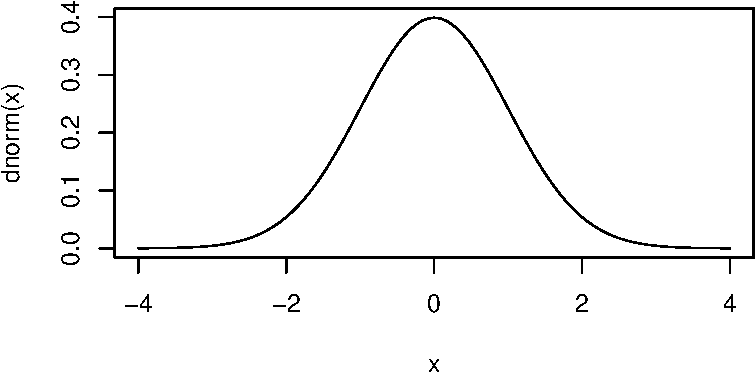
\includegraphics{chapter06_files/figure-pdf/normal-1.pdf}

\begin{Shaded}
\begin{Highlighting}[]
\CommentTok{\# ggplot2を使ってカッコよく}
\FunctionTok{library}\NormalTok{(tidyverse)}
\end{Highlighting}
\end{Shaded}

\begin{verbatim}
-- Attaching core tidyverse packages ------------------------ tidyverse 2.0.0 --
v dplyr     1.1.4     v readr     2.1.4
v forcats   1.0.0     v stringr   1.5.1
v ggplot2   3.4.4     v tibble    3.2.1
v lubridate 1.9.3     v tidyr     1.3.0
v purrr     1.0.2     
-- Conflicts ------------------------------------------ tidyverse_conflicts() --
x dplyr::filter() masks stats::filter()
x dplyr::lag()    masks stats::lag()
i Use the conflicted package (<http://conflicted.r-lib.org/>) to force all conflicts to become errors
\end{verbatim}

\begin{Shaded}
\begin{Highlighting}[]
\FunctionTok{data.frame}\NormalTok{(}\AttributeTok{x =} \FunctionTok{seq}\NormalTok{(}\SpecialCharTok{{-}}\DecValTok{4}\NormalTok{, }\DecValTok{4}\NormalTok{, }\AttributeTok{by =} \FloatTok{0.01}\NormalTok{)) }\SpecialCharTok{\%\textgreater{}\%}
  \FunctionTok{mutate}\NormalTok{(}\AttributeTok{y =} \FunctionTok{dnorm}\NormalTok{(x)) }\SpecialCharTok{\%\textgreater{}\%}
  \FunctionTok{ggplot}\NormalTok{(}\FunctionTok{aes}\NormalTok{(}\AttributeTok{x =}\NormalTok{ x, }\AttributeTok{y =}\NormalTok{ y)) }\SpecialCharTok{+}
  \FunctionTok{geom\_line}\NormalTok{() }\SpecialCharTok{+}
  \FunctionTok{theme\_classic}\NormalTok{()}
\end{Highlighting}
\end{Shaded}

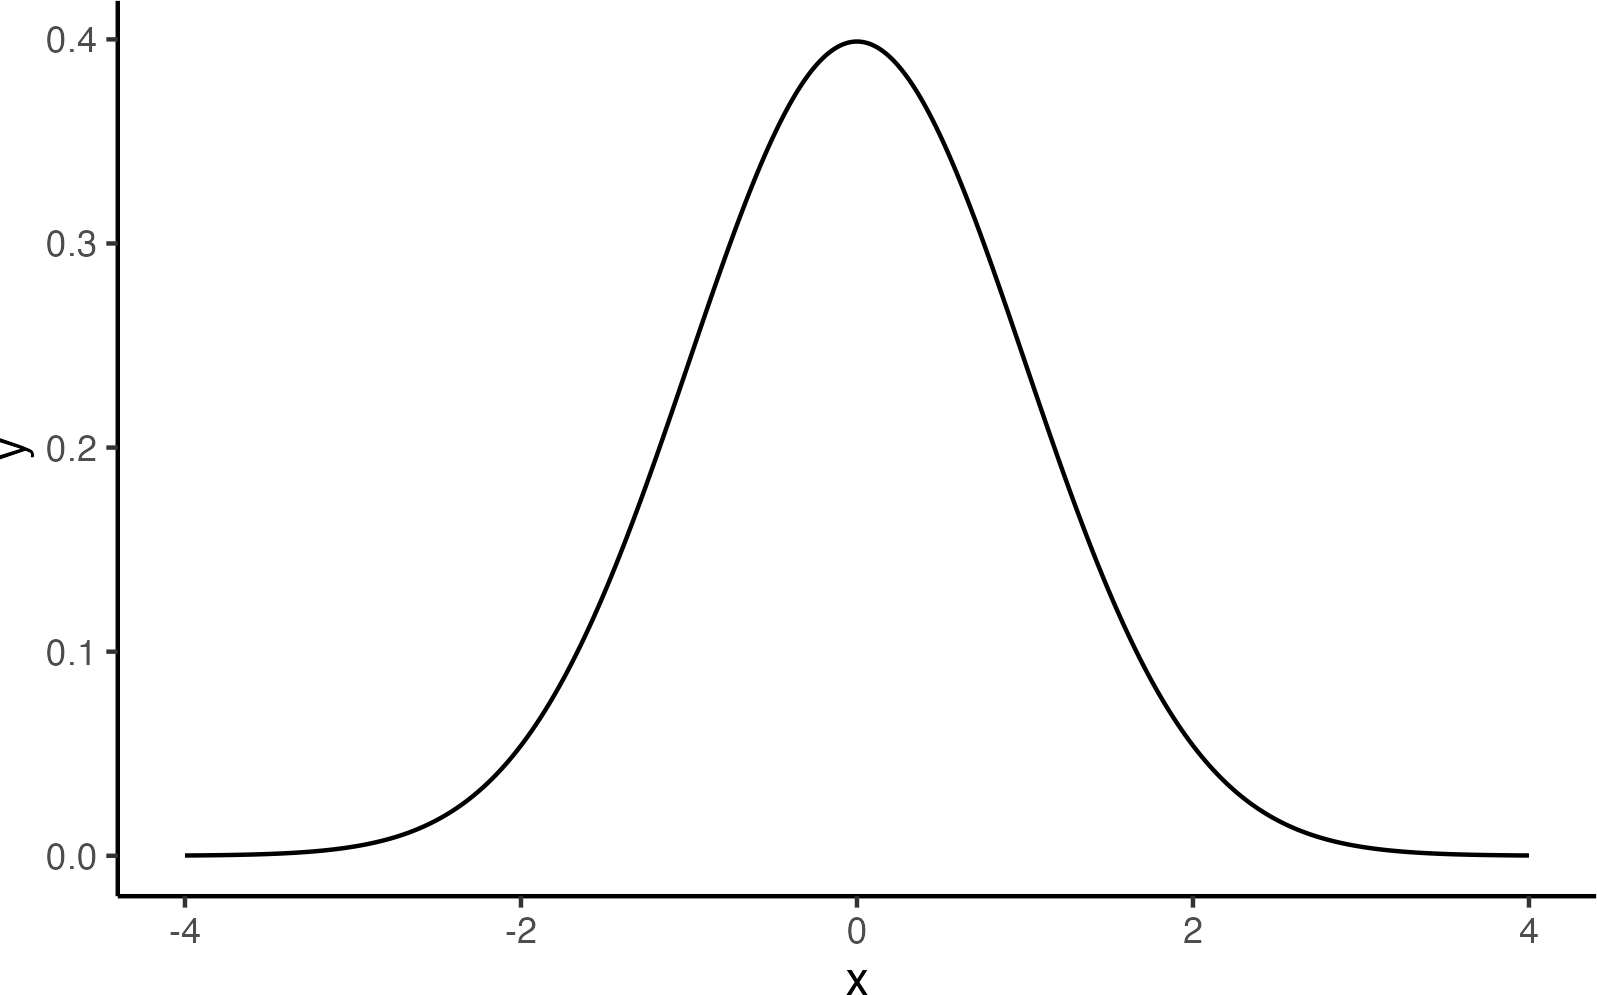
\includegraphics{chapter06_files/figure-pdf/normlByggplot-1.png}

ここで\texttt{dnorm}という関数を使っているが,\texttt{d}はDensity(確率密度)の頭文字であり,\texttt{norm}はNormal
Distribution(正規分布)の一部である。このように,Rでは確率分布の名前を表す名称(ここでは\texttt{norm})と,それに接頭文字ひとつ(\texttt{d})で関数を構成する。この接頭文字は他に\texttt{p},\texttt{q},\texttt{r}があり,\texttt{dpois}(ポアソン分布poisson
distributionの確率密度関数),\texttt{pnorm}(正規分布normal
distributionの累積分布関数),\texttt{rbinom}(二項分布binomial
distributionからの乱数生成)のように使う。

ここでは正規分布を例に説明を続けよう。正規分布は平均\(\mu\)と標準偏差\(\sigma\)でその形状が特徴づけられる。これらの確率分布の特徴を表す数字のことを\textbf{母数
parameter}という。たとえば,次の3つの曲線はパラメータが異なる正規分布である。

\begin{Shaded}
\begin{Highlighting}[]
\FunctionTok{data.frame}\NormalTok{(}\AttributeTok{x =} \FunctionTok{seq}\NormalTok{(}\SpecialCharTok{{-}}\DecValTok{4}\NormalTok{, }\DecValTok{4}\NormalTok{, }\AttributeTok{by =} \FloatTok{0.01}\NormalTok{)) }\SpecialCharTok{\%\textgreater{}\%}
  \FunctionTok{mutate}\NormalTok{(}
    \AttributeTok{y1 =} \FunctionTok{dnorm}\NormalTok{(x, }\AttributeTok{mean =} \DecValTok{0}\NormalTok{, }\AttributeTok{sd =} \DecValTok{1}\NormalTok{),}
    \AttributeTok{y2 =} \FunctionTok{dnorm}\NormalTok{(x, }\AttributeTok{mean =} \DecValTok{1}\NormalTok{, }\AttributeTok{sd =} \FloatTok{0.5}\NormalTok{),}
    \AttributeTok{y3 =} \FunctionTok{dnorm}\NormalTok{(x, }\AttributeTok{mean =} \SpecialCharTok{{-}}\DecValTok{1}\NormalTok{, }\AttributeTok{sd =} \DecValTok{2}\NormalTok{)}
\NormalTok{  ) }\SpecialCharTok{\%\textgreater{}\%}
  \FunctionTok{pivot\_longer}\NormalTok{(}\SpecialCharTok{{-}}\NormalTok{x) }\SpecialCharTok{\%\textgreater{}\%}
  \FunctionTok{ggplot}\NormalTok{(}\FunctionTok{aes}\NormalTok{(}\AttributeTok{x =}\NormalTok{ x, }\AttributeTok{y =}\NormalTok{ value, }\AttributeTok{color =}\NormalTok{ name)) }\SpecialCharTok{+}
  \FunctionTok{geom\_line}\NormalTok{()}
\end{Highlighting}
\end{Shaded}

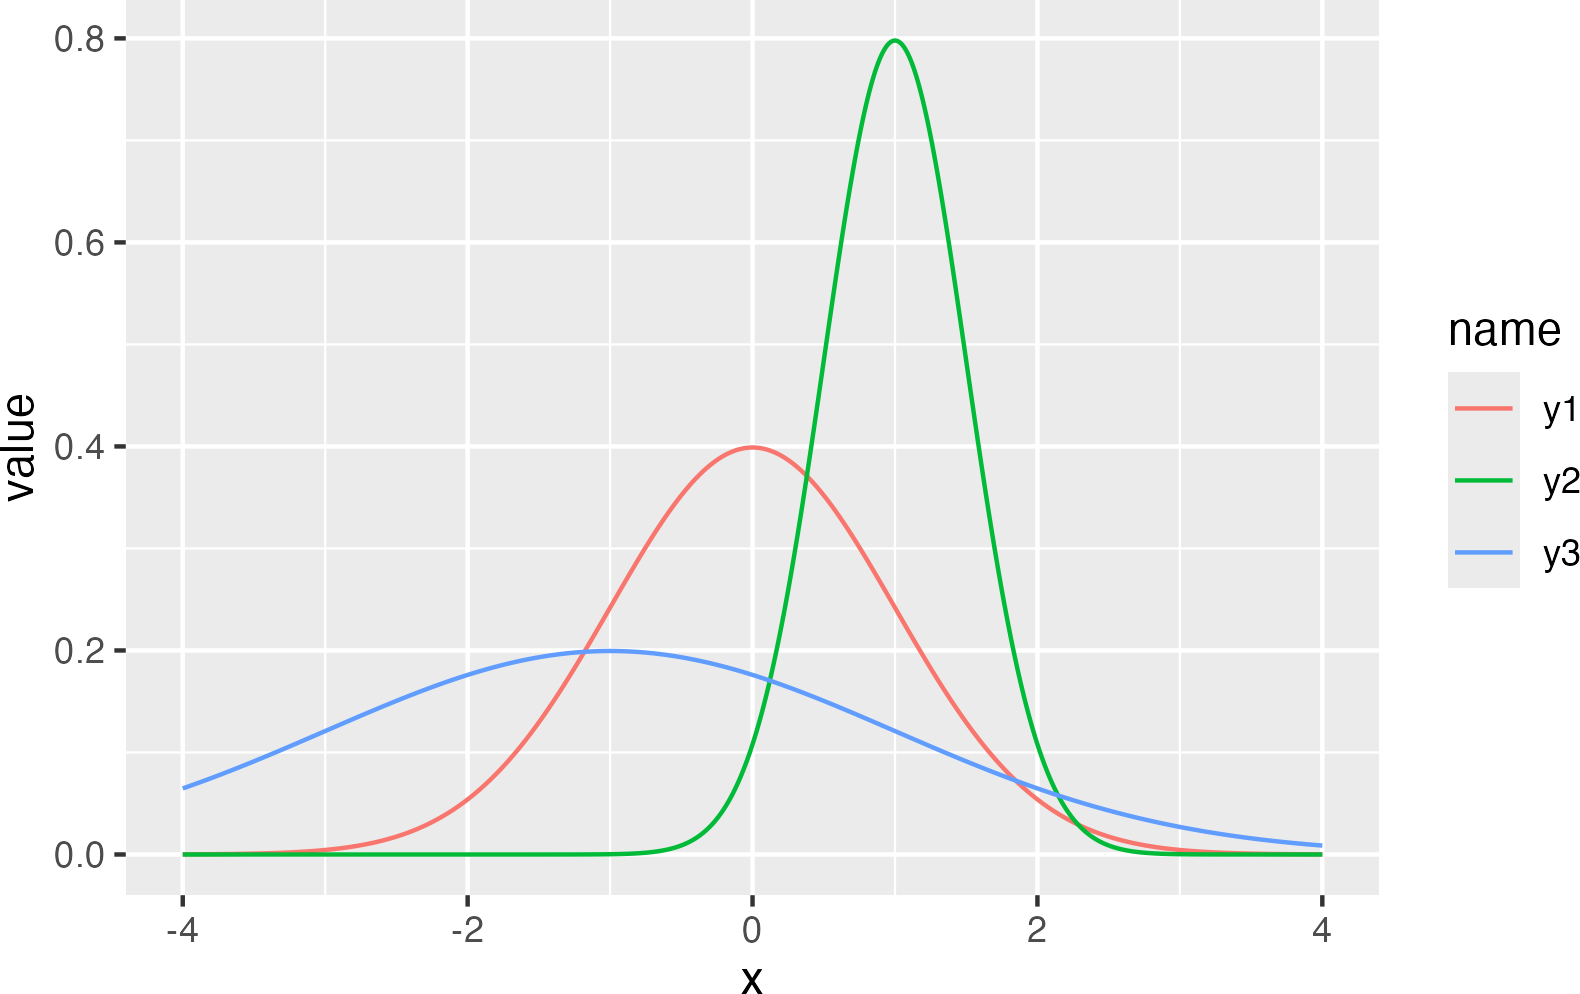
\includegraphics{chapter06_files/figure-pdf/normals-1.png}

平均は位置母数,標準偏差はスケール母数とも呼ばれ,分布の位置と幅を変えていることがわかる。言い換えると,データになるべく当てはまるように正規分布の母数を定めることもできるわけで,左右対称で単峰の分布という特徴があれば,正規分布でかなり様々なパターンを表せる。

さて,上の例で用いた関数はいずれも\texttt{d}を頭に持つ\texttt{dnorm}であり,確率分布の密度の高さを表現していた。では\texttt{p}や\texttt{q}が表すのは何であろうか。数値と図の例を示すので,その対応関係を確認してもらいたい。

\begin{Shaded}
\begin{Highlighting}[]
\CommentTok{\# 累積分布関数}
\FunctionTok{pnorm}\NormalTok{(}\FloatTok{1.96}\NormalTok{, }\AttributeTok{mean =} \DecValTok{0}\NormalTok{, }\AttributeTok{sd =} \DecValTok{1}\NormalTok{)}
\end{Highlighting}
\end{Shaded}

\begin{verbatim}
[1] 0.9750021
\end{verbatim}

\begin{Shaded}
\begin{Highlighting}[]
\CommentTok{\# 累積分布の逆関数}
\FunctionTok{qnorm}\NormalTok{(}\FloatTok{0.975}\NormalTok{, }\AttributeTok{mean =} \DecValTok{0}\NormalTok{, }\AttributeTok{sd =} \DecValTok{1}\NormalTok{)}
\end{Highlighting}
\end{Shaded}

\begin{verbatim}
[1] 1.959964
\end{verbatim}

数値で直感的にわかりにくい場合,次の図を見て確認しよう。\texttt{pnorm}関数はx座標の値を与えると,そこまでの面積(以下のコードで描かれる色付きの領域)すなわち確率を返す。\texttt{qnorm}関数は確率(=面積)を与えると,確率密度関数のカーブの下領域を積分してその値になるときのx座標の値を返す。

\begin{Shaded}
\begin{Highlighting}[]
\CommentTok{\# 描画}
\NormalTok{prob }\OtherTok{\textless{}{-}} \FloatTok{0.9}
\DocumentationTok{\#\# 全体の正規分布カーブ}
\NormalTok{df1 }\OtherTok{\textless{}{-}} \FunctionTok{data.frame}\NormalTok{(}\AttributeTok{x =} \FunctionTok{seq}\NormalTok{(}\AttributeTok{from =} \SpecialCharTok{{-}}\DecValTok{4}\NormalTok{, }\DecValTok{4}\NormalTok{, }\AttributeTok{by =} \FloatTok{0.01}\NormalTok{)) }\SpecialCharTok{\%\textgreater{}\%}
  \FunctionTok{mutate}\NormalTok{(}\AttributeTok{y =} \FunctionTok{dnorm}\NormalTok{(x, }\AttributeTok{mean =} \DecValTok{0}\NormalTok{, }\AttributeTok{sd =} \DecValTok{1}\NormalTok{))}
\DocumentationTok{\#\# qnorm(0.975)までのデータ}
\NormalTok{df2 }\OtherTok{\textless{}{-}} \FunctionTok{data.frame}\NormalTok{(}\AttributeTok{x =} \FunctionTok{seq}\NormalTok{(}\AttributeTok{from =} \SpecialCharTok{{-}}\DecValTok{4}\NormalTok{, }\FunctionTok{qnorm}\NormalTok{(prob), }\AttributeTok{by =} \FloatTok{0.01}\NormalTok{)) }\SpecialCharTok{\%\textgreater{}\%}
  \FunctionTok{mutate}\NormalTok{(}\AttributeTok{y =} \FunctionTok{dnorm}\NormalTok{(x, }\AttributeTok{mean =} \DecValTok{0}\NormalTok{, }\AttributeTok{sd =} \DecValTok{1}\NormalTok{))}
\DocumentationTok{\#\# データセットの違いに注意}
\FunctionTok{ggplot}\NormalTok{() }\SpecialCharTok{+}
  \FunctionTok{geom\_line}\NormalTok{(}\AttributeTok{data =}\NormalTok{ df1, }\FunctionTok{aes}\NormalTok{(}\AttributeTok{x =}\NormalTok{ x, }\AttributeTok{y =}\NormalTok{ y)) }\SpecialCharTok{+}
  \FunctionTok{geom\_ribbon}\NormalTok{(}\AttributeTok{data =}\NormalTok{ df2, }\FunctionTok{aes}\NormalTok{(}\AttributeTok{x =}\NormalTok{ x, }\AttributeTok{y =}\NormalTok{ y, }\AttributeTok{ymin =} \DecValTok{0}\NormalTok{, }\AttributeTok{ymax =}\NormalTok{ y), }\AttributeTok{fill =} \StringTok{"blue"}\NormalTok{, }\AttributeTok{alpha =} \FloatTok{0.3}\NormalTok{) }\SpecialCharTok{+}
  \DocumentationTok{\#\# 以下装飾}
  \FunctionTok{geom\_segment}\NormalTok{(}
    \FunctionTok{aes}\NormalTok{(}\AttributeTok{x =} \FunctionTok{qnorm}\NormalTok{(prob), }\AttributeTok{y =} \FunctionTok{dnorm}\NormalTok{(}\FunctionTok{qnorm}\NormalTok{(prob)), }\AttributeTok{xend =} \FunctionTok{qnorm}\NormalTok{(prob), }\AttributeTok{yend =} \DecValTok{0}\NormalTok{),}
    \AttributeTok{arrow =} \FunctionTok{arrow}\NormalTok{(}\AttributeTok{length =} \FunctionTok{unit}\NormalTok{(}\FloatTok{0.2}\NormalTok{, }\StringTok{"cm"}\NormalTok{)), }\AttributeTok{color =} \StringTok{"red"}
\NormalTok{  )}
\end{Highlighting}
\end{Shaded}

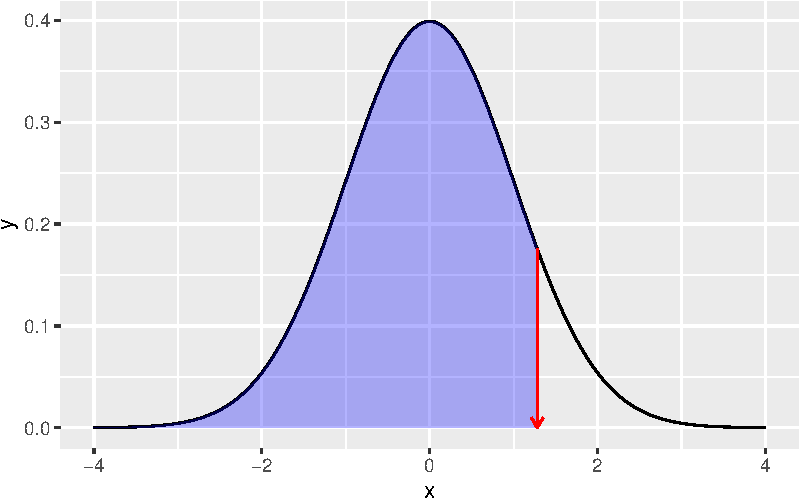
\includegraphics{chapter06_files/figure-pdf/p_qNorm2-1.pdf}

\texttt{d},\texttt{p},\texttt{q},\texttt{r}といった頭の文字は,他の確率分布関数にも付く。では次に\texttt{r}について説明しよう。

\section{乱数}\label{ux4e71ux6570}

乱数とは何であるかを説明するのは,「ランダムである(確率変数である)とは如何なることか」を説明するのと同じように難しい。
カンタンに説明するなら,規則性のない数列という意味である。
しかし計算機はアルゴリズムに沿って正しく数値を計算するものだから,ランダムに,規則性がない数字を示すということは厳密にはあり得ない。
計算機が出す乱数は,乱数生成アルゴリズムに沿って出される数字であり,ランダムに見えて実は規則性があるので,疑似乱数というのが正しい。

とはいえ,人間が適当な数字を思いつきで誦じていく\footnote{厳密なエビデンスは示せないが,俗に「嘘のゴサンパチ」というように人間が適当に数字を述べると5,3,8が使われる率がチャンスレベルより高いと言われている。}よりは,よほど規則性がない数列を出すので,疑似的とはいえ十分に役に立つ。
たとえばアプリなどで「ガチャ」を引くというのは,内部で乱数によって数値を出し,それに基づいてあたり・ハズレ等の判定をしている。他にも,RPGなどで攻撃する時に一定の確率で失敗するとか,一定の確率で「会心の一撃」を出すというのも同様である。ここで大事なのは,そうしたゲームへの実装において規則性のない数字に基づくプログラムにしたとしても,その統計的な性質,すなわち実現値の出現確率はある程度制御したいのである。

そこで,ある確率分布に基づく乱数を生成したい,ということになる。幸いにして,一様乱数(全ての実現値が等しい確率で生じる)を関数で変換することで,正規分布ほか様々な確率分布に従う乱数を作ることができる。Rにはその基本関数として幾つかの確率分布に従う乱数が実装されている。たとえば次のコードは,平均50,SD10の正規分布に従う乱数を10個出現させるものである。

\begin{Shaded}
\begin{Highlighting}[]
\FunctionTok{rnorm}\NormalTok{(}\AttributeTok{n =} \DecValTok{10}\NormalTok{, }\AttributeTok{mean =} \DecValTok{50}\NormalTok{, }\AttributeTok{sd =} \DecValTok{10}\NormalTok{)}
\end{Highlighting}
\end{Shaded}

\begin{verbatim}
 [1] 43.17577 47.41263 54.22270 66.96133 64.52274 54.68405 52.35370 41.71688
 [9] 62.32527 61.63775
\end{verbatim}

たとえば諸君が心理統計の練習問題を作ろうとして,適当な数列が欲しければこのようにすれば良いかもしれない。しかし,同じ問題をもう一度作ろうとすると,乱数なのでまた違う数字が出てしまう。

\begin{Shaded}
\begin{Highlighting}[]
\FunctionTok{rnorm}\NormalTok{(}\AttributeTok{n =} \DecValTok{10}\NormalTok{, }\AttributeTok{mean =} \DecValTok{50}\NormalTok{, }\AttributeTok{sd =} \DecValTok{10}\NormalTok{)}
\end{Highlighting}
\end{Shaded}

\begin{verbatim}
 [1] 55.13995 33.92545 38.51067 42.08051 54.22726 40.26258 47.29947 38.26302
 [9] 40.60522 49.55872
\end{verbatim}

疑似乱数に過ぎないのだから,再現性のある乱数を生じさせたいと思うかもしれない。そのような場合は,\texttt{set.seed}関数を使う。疑似乱数は内部の乱数生成の種(seed)から計算して作られているため,その数字を固定してやると同じ乱数が再現できる。

\begin{Shaded}
\begin{Highlighting}[]
\CommentTok{\# seedを指定}
\FunctionTok{set.seed}\NormalTok{(}\DecValTok{12345}\NormalTok{)}
\FunctionTok{rnorm}\NormalTok{(}\AttributeTok{n =} \DecValTok{3}\NormalTok{)}
\end{Highlighting}
\end{Shaded}

\begin{verbatim}
[1]  0.5855288  0.7094660 -0.1093033
\end{verbatim}

\begin{Shaded}
\begin{Highlighting}[]
\CommentTok{\# 同じseedを再設定}
\FunctionTok{set.seed}\NormalTok{(}\DecValTok{12345}\NormalTok{)}
\FunctionTok{rnorm}\NormalTok{(}\AttributeTok{n =} \DecValTok{3}\NormalTok{)}
\end{Highlighting}
\end{Shaded}

\begin{verbatim}
[1]  0.5855288  0.7094660 -0.1093033
\end{verbatim}

\subsection{乱数のつかいかた}\label{ux4e71ux6570ux306eux3064ux304bux3044ux304bux305f}

乱数の使い方のひとつは,先に述べたように,プログラムが偶然による振る舞いをしているように仕掛けたいとき,ということだろう。

実は他にも使い道がある。それは確率分布を具体的に知りたいときである。次に示すのは,標準正規分布から\(n = 10,100,1000,10000\)とした時のヒストグラムである。

\begin{Shaded}
\begin{Highlighting}[]
\NormalTok{rN10 }\OtherTok{\textless{}{-}} \FunctionTok{rnorm}\NormalTok{(}\DecValTok{10}\NormalTok{)}
\NormalTok{rN100 }\OtherTok{\textless{}{-}} \FunctionTok{rnorm}\NormalTok{(}\DecValTok{100}\NormalTok{)}
\NormalTok{rN1000 }\OtherTok{\textless{}{-}} \FunctionTok{rnorm}\NormalTok{(}\DecValTok{1000}\NormalTok{)}
\NormalTok{rN10000 }\OtherTok{\textless{}{-}} \FunctionTok{rnorm}\NormalTok{(}\DecValTok{10000}\NormalTok{)}

\FunctionTok{data.frame}\NormalTok{(}
  \AttributeTok{N =} \FunctionTok{c}\NormalTok{(}
    \FunctionTok{rep}\NormalTok{(}\DecValTok{1}\NormalTok{, }\DecValTok{10}\NormalTok{), }\FunctionTok{rep}\NormalTok{(}\DecValTok{2}\NormalTok{, }\DecValTok{100}\NormalTok{),}
    \FunctionTok{rep}\NormalTok{(}\DecValTok{3}\NormalTok{, }\DecValTok{1000}\NormalTok{), }\FunctionTok{rep}\NormalTok{(}\DecValTok{4}\NormalTok{, }\DecValTok{10000}\NormalTok{)}
\NormalTok{  ),}
  \AttributeTok{X =} \FunctionTok{c}\NormalTok{(rN10, rN100, rN1000, rN10000)}
\NormalTok{) }\SpecialCharTok{\%\textgreater{}\%}
  \FunctionTok{mutate}\NormalTok{(}\AttributeTok{N =} \FunctionTok{as.factor}\NormalTok{(N)) }\SpecialCharTok{\%\textgreater{}\%}
  \FunctionTok{ggplot}\NormalTok{(}\FunctionTok{aes}\NormalTok{(}\AttributeTok{x =}\NormalTok{ X, }\AttributeTok{fill =}\NormalTok{ N)) }\SpecialCharTok{+}
  \CommentTok{\# 縦軸を相対頻度に}
  \FunctionTok{geom\_histogram}\NormalTok{(}\FunctionTok{aes}\NormalTok{(}\AttributeTok{y =}\NormalTok{ ..density..)) }\SpecialCharTok{+}
  \FunctionTok{facet\_wrap}\NormalTok{(}\SpecialCharTok{\textasciitilde{}}\NormalTok{N)}
\end{Highlighting}
\end{Shaded}

\begin{verbatim}
Warning: The dot-dot notation (`..density..`) was deprecated in ggplot2 3.4.0.
i Please use `after_stat(density)` instead.
\end{verbatim}

\begin{verbatim}
`stat_bin()` using `bins = 30`. Pick better value with `binwidth`.
\end{verbatim}

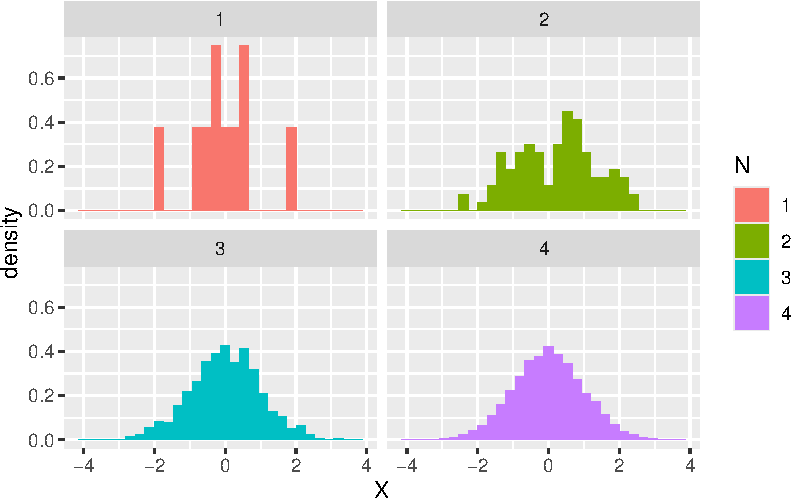
\includegraphics{chapter06_files/figure-pdf/rnorm-1.pdf}

これを見ると,最初の10個程度のヒストグラムは不規則な分布に見えるが,100,1000と増えるに従って徐々に正規分布の理論的形状に近似していくところがみて取れる。

Rにはポアソン分布や二項分布などに加え,統計に馴染みの深いt分布やF分布,\(\chi^2\)分布などの確率分布関数も実装されている。これらの分布はパラメタの値を聞いてもイメージしにくいところがあるかもしれないが,そのような時はパラメタを指定した上で乱数を大量に生成し,そのヒストグラムを描けば確率分布関数の形が眼に見えてくるため,より具体的に理解できるだろう。

実際,ベイズ統計学が昨今隆盛している一つの理由は,計算機科学の貢献によるところが大きい。\textbf{マルコフ連鎖モンテカルロ法}(MCMC法)と呼ばれる乱数発生技術は,明確な名前を持たないモデルによって作られる事後分布からでも,乱数を生成できる技術である。この分布は解析的に示すことは困難であるが,そこから乱数を生成し,そのヒストグラムを見ることで,形状を可視化できるのである。

また,この乱数利用法の利点は可視化だけではない。標準正規分布において,ある範囲の面積(=確率)が知りたいとする。たとえば,確率点-1.5から+1.5までの範囲の面積を求めたいとしよう。正規分布の数式はわかっているので,次のようにすればその面積は求められる。
\[ p = \int_{-1.5}^{+1.5} \frac{1}{\sqrt{2\pi}}e^{-\frac{x^2}{2}} dx \]

もちろん我々は\texttt{pnorm}関数を知っているので,次のようにして数値解を得ることができる。

\begin{Shaded}
\begin{Highlighting}[]
\FunctionTok{pnorm}\NormalTok{(}\SpecialCharTok{+}\FloatTok{1.5}\NormalTok{, }\AttributeTok{mean =} \DecValTok{0}\NormalTok{, }\AttributeTok{sd =} \DecValTok{1}\NormalTok{) }\SpecialCharTok{{-}} \FunctionTok{pnorm}\NormalTok{(}\SpecialCharTok{{-}}\FloatTok{1.5}\NormalTok{, }\AttributeTok{mean =} \DecValTok{0}\NormalTok{, }\AttributeTok{sd =} \DecValTok{1}\NormalTok{)}
\end{Highlighting}
\end{Shaded}

\begin{verbatim}
[1] 0.8663856
\end{verbatim}

同様のことは乱数を使って,次のように近似解を得ることができる。

\begin{Shaded}
\begin{Highlighting}[]
\NormalTok{x }\OtherTok{\textless{}{-}} \FunctionTok{rnorm}\NormalTok{(}\DecValTok{100000}\NormalTok{, }\AttributeTok{mean =} \DecValTok{0}\NormalTok{, }\AttributeTok{sd =} \DecValTok{1}\NormalTok{)}
\NormalTok{df }\OtherTok{\textless{}{-}} \FunctionTok{data.frame}\NormalTok{(}\AttributeTok{X =}\NormalTok{ x) }\SpecialCharTok{\%\textgreater{}\%}
  \CommentTok{\# 該当する範囲かどうかを判定する変数を作る}
  \FunctionTok{mutate}\NormalTok{(}\AttributeTok{FLG =} \FunctionTok{ifelse}\NormalTok{(X }\SpecialCharTok{\textgreater{}} \SpecialCharTok{{-}}\FloatTok{1.5} \SpecialCharTok{\&}\NormalTok{ X }\SpecialCharTok{\textless{}} \FloatTok{1.5}\NormalTok{, }\DecValTok{1}\NormalTok{, }\DecValTok{2}\NormalTok{)) }\SpecialCharTok{\%\textgreater{}\%}
  \FunctionTok{mutate}\NormalTok{(}\AttributeTok{FLG =} \FunctionTok{factor}\NormalTok{(FLG, }\AttributeTok{labels =} \FunctionTok{c}\NormalTok{(}\StringTok{"in"}\NormalTok{, }\StringTok{"out"}\NormalTok{)))}
\DocumentationTok{\#\# 計算}
\NormalTok{df }\SpecialCharTok{\%\textgreater{}\%}
  \FunctionTok{group\_by}\NormalTok{(FLG) }\SpecialCharTok{\%\textgreater{}\%}
  \FunctionTok{summarise}\NormalTok{(}\AttributeTok{n =} \FunctionTok{n}\NormalTok{()) }\SpecialCharTok{\%\textgreater{}\%}
  \FunctionTok{mutate}\NormalTok{(}\AttributeTok{prob =}\NormalTok{ n }\SpecialCharTok{/} \DecValTok{100000}\NormalTok{)}
\end{Highlighting}
\end{Shaded}

\begin{verbatim}
# A tibble: 2 x 3
  FLG       n  prob
  <fct> <int> <dbl>
1 in    86642 0.866
2 out   13358 0.134
\end{verbatim}

ここでは乱数を10,000個生成し,指定の範囲内に入るかどうか(入れば1,入らなければ2)を示すfactor型変数\texttt{FLG}を作った。この変数ごとに群分けして数を数え,総数で割ることで相対度数にする。確率は全体の中に占める相対的な面積の割合であり,今回当該領域の値が\texttt{0.866}と\texttt{pnorm}関数で算出した解とほぼ同等の値変えられている。

なお,次のようにすれば範囲の可視化も容易い。

\begin{Shaded}
\begin{Highlighting}[]
\DocumentationTok{\#\# 可視化}
\NormalTok{df }\SpecialCharTok{\%\textgreater{}\%}
  \FunctionTok{ggplot}\NormalTok{(}\FunctionTok{aes}\NormalTok{(}\AttributeTok{x =}\NormalTok{ X, }\AttributeTok{fill =}\NormalTok{ FLG)) }\SpecialCharTok{+}
  \FunctionTok{geom\_histogram}\NormalTok{(}\AttributeTok{binwidth =} \FloatTok{0.01}\NormalTok{)}
\end{Highlighting}
\end{Shaded}

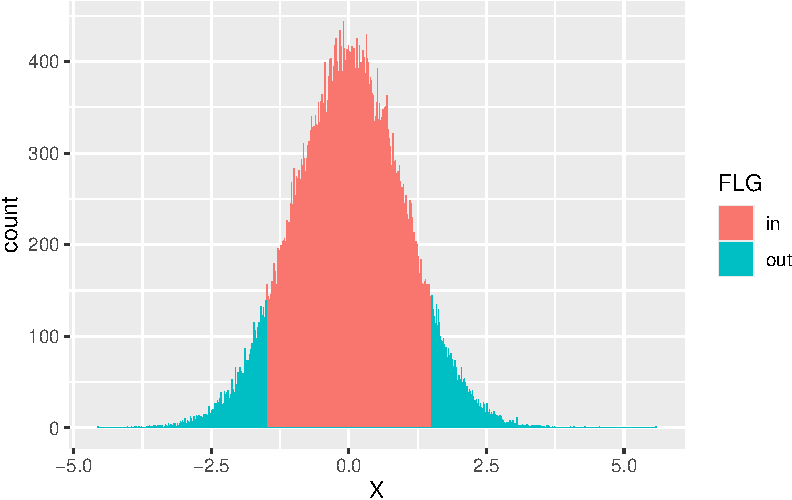
\includegraphics{chapter06_files/figure-pdf/norm_vis-1.pdf}

繰り返すが,確率分布の形がイメージできなかったり,解析的にその式を書き表すことが困難であった場合でも,具体的な数値にすることでヒストグラムで可視化でき,また近似的に確率計算ができている。

あくまでも近似に過ぎないのでその精度が信用できない,というひとは生成する乱数の数を10倍,100倍にすれば良い。昨今の計算機の計算能力において,その程度の増加はさほど計算料の負担にならない。複雑な積分計算が記述統計量(数え上げ)の問題になる点で,具体的に理解できるという利点は大きい。

さらに思いを馳せてほしいのだが,心理学者は心理学実験や調査によって,データを得る。しかしそれらは個人差や誤差を考え,確率変数だとされている。目の前の数件から数十件のデータであっても,正規分布に従うと仮定して統計的処理をおこなう。これは「乱数によって生成したデータ」に対して行うとしても本質的には同じである。すなわち,調査実験を行う前に,乱数によってシミュレーションしておくことができるのである。調査実験の本番一発勝負をする前に,自分の取ろうとしているデータがどのような性質を持ちうるかを具体的に確かめておくことは重要な試みであろう。

\section{練習問題;乱数を用いて}\label{ux7df4ux7fd2ux554fux984cux4e71ux6570ux3092ux7528ux3044ux3066}

正規乱数を用いて,次の値を近似計算してみよう。なお設定や解析的に算出した「真の値」と少数以下2位までの精度が得られるように工夫しよう。

\begin{enumerate}
\def\labelenumi{\arabic{enumi}.}
\tightlist
\item
  平均100,標準偏差8の正規分布の期待値。なお連続確率変数の期待値は次の式で表されます。\[E[X] = \int_{-\infty}^{\infty} x f(x) \, dx\]
  ここで\(x\)は確率変数を表し,\(f(x)\)は確率密度関数であり,確率密度関数の全定義域を積分することで得られます。正規分布の期待値は,平均パラメータに一致しますので,今回の真値は設定した\(100\)になります。
\item
  平均100,標準偏差3の正規分布の分散を計算してみよう。なお連続確率変数の分散は次の式で表されます。\[\sigma^2 = \int_{-\infty}^{\infty} (x - \mu)^2 f(x) \, dx\]
  ここで\(\mu\)は確率変数の期待値であり,正規分布の分散は,標準偏差パラメータの二乗に一致しますので,今回の真値は\(3^2 = 9\)です。
\item
  平均65,標準偏差10の正規分布に従う確率変数\(X\)の,\(90 < X < 110\)の面積。解析的に計算した結果は次の通りです。
\end{enumerate}

\begin{Shaded}
\begin{Highlighting}[]
\FunctionTok{pnorm}\NormalTok{(}\DecValTok{108}\NormalTok{, }\AttributeTok{mean =} \DecValTok{65}\NormalTok{, }\AttributeTok{sd =} \DecValTok{10}\NormalTok{) }\SpecialCharTok{{-}} \FunctionTok{pnorm}\NormalTok{(}\DecValTok{92}\NormalTok{, }\AttributeTok{mean =} \DecValTok{65}\NormalTok{, }\AttributeTok{sd =} \DecValTok{10}\NormalTok{)}
\end{Highlighting}
\end{Shaded}

\begin{verbatim}
[1] 0.003458434
\end{verbatim}

\begin{enumerate}
\def\labelenumi{\arabic{enumi}.}
\setcounter{enumi}{3}
\tightlist
\item
  平均10,標準偏差10の正規分布において,実現値が7以上になる確率。解析的に計算した結果は次の通りです。
\end{enumerate}

\begin{Shaded}
\begin{Highlighting}[]
\DecValTok{1} \SpecialCharTok{{-}} \FunctionTok{pnorm}\NormalTok{(}\DecValTok{7}\NormalTok{, }\AttributeTok{mean =} \DecValTok{10}\NormalTok{, }\AttributeTok{sd =} \DecValTok{10}\NormalTok{)}
\end{Highlighting}
\end{Shaded}

\begin{verbatim}
[1] 0.6179114
\end{verbatim}

\begin{enumerate}
\def\labelenumi{\arabic{enumi}.}
\setcounter{enumi}{4}
\tightlist
\item
  確率変数\(X,Y\)があります。\(X\)は平均10,SD10の正規分布,\(Y\)は平均5,SD8の正規分布に従うものとします。ここで,\(X\)と\(Y\)が独立であるとしたとき,和\(Z=X+Y\)の平均と分散が,もとの\(X,Y\)の平均の和,分散の和になっていることを,乱数を使って確認してください。
\end{enumerate}

\section{母集団と標本}\label{ux6bcdux96c6ux56e3ux3068ux6a19ux672c}

ここまで確率分布の性質を見るために乱数を利用する方法を見てきた。ここからは,推測統計学における確率分布の利用を考える。推測統計では,知りたい集団全体のことを\textbf{母集団population},そこから得られた一部のデータを\textbf{標本sample}と呼ぶのであった。標本の統計量を使って,母集団の性質を推論するのが推測統計/統計的推測である。母集団の特徴を表す統計量は\textbf{母数parameter}と呼ばれ,母平均,母分散など「母」の字をつけて母集団の情報であることを示す。同様に,標本の平均や分散も計算できるが,この時は標本平均,標本分散など「標本」をつけて明示的に違いを強調することもある。

乱数を使って具体的な例で見てみよう。ここに100人から構成される村があったとする。この村の人々の身長を測ってデータにしたとしよう。100個の適当な数字を考えるのは面倒なので,乱数で生成してこれに代える。

\begin{Shaded}
\begin{Highlighting}[]
\FunctionTok{set.seed}\NormalTok{(}\DecValTok{12345}\NormalTok{)}
\CommentTok{\# 100人分の身長データをつくる。小数点以下2桁を丸めた}
\NormalTok{Po }\OtherTok{\textless{}{-}} \FunctionTok{rnorm}\NormalTok{(}\DecValTok{100}\NormalTok{, }\AttributeTok{mean =} \DecValTok{150}\NormalTok{, }\AttributeTok{sd =} \DecValTok{10}\NormalTok{) }\SpecialCharTok{\%\textgreater{}\%} \FunctionTok{round}\NormalTok{(}\DecValTok{2}\NormalTok{)}
\FunctionTok{print}\NormalTok{(Po)}
\end{Highlighting}
\end{Shaded}

\begin{verbatim}
  [1] 155.86 157.09 148.91 145.47 156.06 131.82 156.30 147.24 147.16 140.81
 [11] 148.84 168.17 153.71 155.20 142.49 158.17 141.14 146.68 161.21 152.99
 [21] 157.80 164.56 143.56 134.47 134.02 168.05 145.18 156.20 156.12 148.38
 [31] 158.12 171.97 170.49 166.32 152.54 154.91 146.76 133.38 167.68 150.26
 [41] 161.29 126.20 139.40 159.37 158.54 164.61 135.87 155.67 155.83 136.93
 [51] 144.60 169.48 150.54 153.52 143.29 152.78 156.91 158.24 171.45 126.53
 [61] 151.50 136.57 155.53 165.90 144.13 131.68 158.88 165.93 155.17 137.04
 [71] 150.55 142.15 139.51 173.31 164.03 159.43 158.26 141.88 154.76 160.21
 [81] 156.45 160.43 146.96 174.77 159.71 168.67 156.72 146.92 155.37 158.25
 [91] 140.36 141.45 168.87 146.08 140.19 156.87 144.95 171.58 144.00 143.05
\end{verbatim}

この100人の村が母集団なので,母平均や母分散は次のようにして計算できる。

\begin{Shaded}
\begin{Highlighting}[]
\NormalTok{M }\OtherTok{\textless{}{-}} \FunctionTok{mean}\NormalTok{(Po)}
\NormalTok{V }\OtherTok{\textless{}{-}} \FunctionTok{mean}\NormalTok{((Po }\SpecialCharTok{{-}}\NormalTok{ M)}\SpecialCharTok{\^{}}\DecValTok{2}\NormalTok{)}
\CommentTok{\# 母平均}
\FunctionTok{print}\NormalTok{(M)}
\end{Highlighting}
\end{Shaded}

\begin{verbatim}
[1] 152.4521
\end{verbatim}

\begin{Shaded}
\begin{Highlighting}[]
\CommentTok{\# 母分散}
\FunctionTok{print}\NormalTok{(V)}
\end{Highlighting}
\end{Shaded}

\begin{verbatim}
[1] 123.0206
\end{verbatim}

さて,この村からランダムに10人の標本を得たとしよう。ベクトルの前から10人でも良いが,Rにはサンプリングをする関数\texttt{sample}があるのでこれを活用したい。

\begin{Shaded}
\begin{Highlighting}[]
\NormalTok{s1 }\OtherTok{\textless{}{-}} \FunctionTok{sample}\NormalTok{(Po, }\AttributeTok{size =} \DecValTok{10}\NormalTok{)}
\NormalTok{s1}
\end{Highlighting}
\end{Shaded}

\begin{verbatim}
 [1] 164.61 155.86 136.93 143.29 160.43 168.87 151.50 155.17 153.71 135.87
\end{verbatim}

この\texttt{s1}が手元のデータである。心理学の実験でデータを得る,というのはこのように全体に対してごく一部だけ取り出したものになる。このサンプルの平均や分散は標本平均,標本分散である。

\begin{Shaded}
\begin{Highlighting}[]
\NormalTok{m1 }\OtherTok{\textless{}{-}} \FunctionTok{mean}\NormalTok{(s1)}
\NormalTok{v1 }\OtherTok{\textless{}{-}} \FunctionTok{mean}\NormalTok{((s1 }\SpecialCharTok{{-}} \FunctionTok{mean}\NormalTok{(s1))}\SpecialCharTok{\^{}}\DecValTok{2}\NormalTok{)}
\CommentTok{\# 標本平均}
\FunctionTok{print}\NormalTok{(m1)}
\end{Highlighting}
\end{Shaded}

\begin{verbatim}
[1] 152.624
\end{verbatim}

\begin{Shaded}
\begin{Highlighting}[]
\CommentTok{\# 標本分散}
\FunctionTok{print}\NormalTok{(v1)}
\end{Highlighting}
\end{Shaded}

\begin{verbatim}
[1] 110.2049
\end{verbatim}

今回,母平均は152.4521で標本平均は152.624である。実際に知りうる値は標本の値だけなので,標本平均152.624を得たら,母平均も152.624に近い値だろうな,と推測するのはおかしなことではないだろう。しかし標本平均は,標本の取り方によって毎回変わるものである。試しにもう一つ,標本をとったとしよう。

\begin{Shaded}
\begin{Highlighting}[]
\NormalTok{s2 }\OtherTok{\textless{}{-}} \FunctionTok{sample}\NormalTok{(Po, }\AttributeTok{size =} \DecValTok{10}\NormalTok{)}
\NormalTok{s2}
\end{Highlighting}
\end{Shaded}

\begin{verbatim}
 [1] 154.76 135.87 143.05 171.45 136.57 170.49 156.87 158.25 155.17 155.20
\end{verbatim}

\begin{Shaded}
\begin{Highlighting}[]
\NormalTok{m2 }\OtherTok{\textless{}{-}} \FunctionTok{mean}\NormalTok{(s2)}
\NormalTok{v2 }\OtherTok{\textless{}{-}} \FunctionTok{mean}\NormalTok{((s2 }\SpecialCharTok{{-}} \FunctionTok{mean}\NormalTok{(s2))}\SpecialCharTok{\^{}}\DecValTok{2}\NormalTok{)}
\CommentTok{\# 標本平均その2}
\FunctionTok{print}\NormalTok{(m2)}
\end{Highlighting}
\end{Shaded}

\begin{verbatim}
[1] 153.768
\end{verbatim}

今回の標本平均は153.768になった。このデータが得られたら,諸君は母平均が「153.768に近い値だろうな」と推測するに違いない。標本1の152.624と標本2の153.768を比べると,前者の方が正解152.4521に近い(その差はそれぞれ-0.1719と-1.3159である)。つまり,標本の取り方によっては当たり外れがあるということである。データをとって研究していても,仮説を支持する結果なのかそうでないのかは,こうした確率的揺らぎの下にある。

つまり,\textbf{標本は確率変数であり,標本統計量も確率的に変わりうる}ものである。標本統計量でもって母数を推定するときは,標本統計量の性質や標本統計量が従う確率分布を知っておく必要がある。以下では母数の推定に望ましい性質を持つ推定量の望ましい性質をみていこう。

\section{一致性}\label{ux4e00ux81f4ux6027}

最も単純には,標本統計量が母数に近ければ近いほど,できれば一致してくれれば喜ばしい。先ほどの例では100人の村から10人しか取り出さなかったが,もし20人,30人とサンプルサイズが大きくなると母数に近づいていくことが予想できる。この性質のことを\textbf{一致性}consistencyといい,推定量が持っていてほしい性質のひとつである。幸い,標本平均は母平均に対して一致性を持っている。

このことを確認してみよう。サンプルサイズを様々に変えて計算してみれば良い。例として,平均50,SD10の正規分布からサンプルサイズを2から1000まで増やしていくことにしよう。サンプルを取り出すことを,乱数生成に置き換えてその平均を計算していくこととする。

\begin{Shaded}
\begin{Highlighting}[]
\FunctionTok{set.seed}\NormalTok{(}\DecValTok{12345}\NormalTok{)}
\NormalTok{sample\_size }\OtherTok{\textless{}{-}} \FunctionTok{seq}\NormalTok{(}\AttributeTok{from =} \DecValTok{2}\NormalTok{, }\AttributeTok{to =} \DecValTok{1000}\NormalTok{, }\AttributeTok{by =} \DecValTok{10}\NormalTok{)}
\CommentTok{\# 平均値を格納するオブジェクトを初期化}
\NormalTok{sample\_mean }\OtherTok{\textless{}{-}} \FunctionTok{rep}\NormalTok{(}\DecValTok{0}\NormalTok{, }\FunctionTok{length}\NormalTok{(sample\_size))}
\CommentTok{\# 反復}
\ControlFlowTok{for}\NormalTok{ (i }\ControlFlowTok{in} \DecValTok{1}\SpecialCharTok{:}\FunctionTok{length}\NormalTok{(sample\_size)) \{}
\NormalTok{  sample\_mean[i] }\OtherTok{\textless{}{-}} \FunctionTok{rnorm}\NormalTok{(sample\_size[i], }\AttributeTok{mean =} \DecValTok{50}\NormalTok{, }\AttributeTok{sd =} \DecValTok{10}\NormalTok{) }\SpecialCharTok{\%\textgreater{}\%}
    \FunctionTok{mean}\NormalTok{()}
\NormalTok{\}}

\CommentTok{\# 可視化}
\FunctionTok{data.frame}\NormalTok{(}\AttributeTok{size =}\NormalTok{ sample\_size, }\AttributeTok{M =}\NormalTok{ sample\_mean) }\SpecialCharTok{\%\textgreater{}\%}
  \FunctionTok{ggplot}\NormalTok{(}\FunctionTok{aes}\NormalTok{(}\AttributeTok{x =}\NormalTok{ size, }\AttributeTok{y =}\NormalTok{ M)) }\SpecialCharTok{+}
  \FunctionTok{geom\_point}\NormalTok{() }\SpecialCharTok{+}
  \FunctionTok{geom\_line}\NormalTok{() }\SpecialCharTok{+}
  \FunctionTok{geom\_hline}\NormalTok{(}\AttributeTok{yintercept =} \DecValTok{50}\NormalTok{, }\AttributeTok{color =} \StringTok{"red"}\NormalTok{)}
\end{Highlighting}
\end{Shaded}

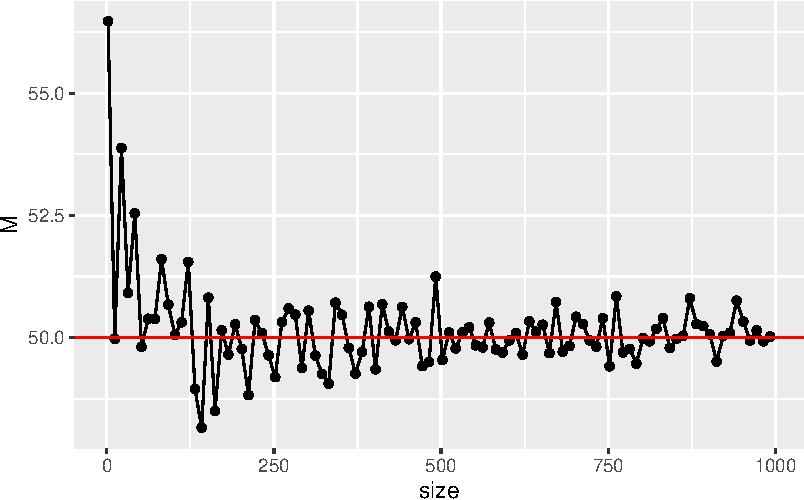
\includegraphics{chapter06_files/figure-pdf/consistency-1.pdf}

このようにサンプルサイズが増えていくにつれて,真値の50に近づいていくことが見て取れる。母集団分布の形状やパラメータ,サンプルサイズなどを変えて確認してみよう。

\section{不偏性}\label{ux4e0dux504fux6027}

推定量は確率変数であり,確率分布でその性質を記述することができる。標本統計量の従う確率分布のことを\textbf{標本分布}と呼ぶが,標本分布の確率密度関数がわかっているなら,その期待値や分散も計算できるだろう。推定量の期待値(平均)が母数に一致することも,推定量の望ましい性質の一つであり,この性質のことを\textbf{不偏性}unbiasednessという。

心理統計を学ぶ時に初学者を苛立たせるステップの一つとして,分散の計算の時にサンプルサイズ\(n\)ではなく\(n-1\)で割る,という操作がある。これは不偏分散といって標本分散とは違うのだが,前者が不偏性を持っているのに対し,後者がそうでないからである。これを乱数を使って確認してみよう。

平均50,SD10(母分散\(10^2=100\))の母集団から,サンプルサイズ\(n=20\)の標本を繰り返し得る。これはサイズ20の乱数生成で行う。各標本に対して標本分散と不偏分散を計算し,その平均(標本統計量の期待値)を計算してみよう。

\begin{Shaded}
\begin{Highlighting}[]
\NormalTok{iter }\OtherTok{\textless{}{-}} \DecValTok{5000}
\NormalTok{vars }\OtherTok{\textless{}{-}} \FunctionTok{rep}\NormalTok{(}\DecValTok{0}\NormalTok{, iter)}
\NormalTok{unbiased\_vars }\OtherTok{\textless{}{-}} \FunctionTok{rep}\NormalTok{(}\DecValTok{0}\NormalTok{, iter)}

\DocumentationTok{\#\# 乱数の生成と計算}
\FunctionTok{set.seed}\NormalTok{(}\DecValTok{12345}\NormalTok{)}
\ControlFlowTok{for}\NormalTok{ (i }\ControlFlowTok{in} \DecValTok{1}\SpecialCharTok{:}\NormalTok{iter) \{}
\NormalTok{  sample }\OtherTok{\textless{}{-}} \FunctionTok{rnorm}\NormalTok{(}\AttributeTok{n =} \DecValTok{20}\NormalTok{, }\AttributeTok{mean =} \DecValTok{50}\NormalTok{, }\AttributeTok{sd =} \DecValTok{10}\NormalTok{)}
\NormalTok{  vars[i] }\OtherTok{\textless{}{-}} \FunctionTok{mean}\NormalTok{((sample }\SpecialCharTok{{-}} \FunctionTok{mean}\NormalTok{(sample))}\SpecialCharTok{\^{}}\DecValTok{2}\NormalTok{)}
\NormalTok{  unbiased\_vars[i] }\OtherTok{\textless{}{-}} \FunctionTok{var}\NormalTok{(sample)}
\NormalTok{\}}

\DocumentationTok{\#\# 期待値}
\FunctionTok{mean}\NormalTok{(vars)}
\end{Highlighting}
\end{Shaded}

\begin{verbatim}
[1] 95.08531
\end{verbatim}

\begin{Shaded}
\begin{Highlighting}[]
\FunctionTok{mean}\NormalTok{(unbiased\_vars)}
\end{Highlighting}
\end{Shaded}

\begin{verbatim}
[1] 100.0898
\end{verbatim}

標本分散を計算したオブジェクト\texttt{vars}の平均すなわち期待値は95.0853144であり,設定した値(真値)の100からは幾分はなれている。これに対して,Rの埋め込み関数である\texttt{var}をつかった不偏分散の平均すなわち期待値は100.0898047であり,母分散の推定量としてはこちらの方が好ましいことがわかる。このように標本分散にはバイアスが生じることがわかっているので,あらかじめバイアスを補正するために元の計算式を修正していたのである。この説明で,苛立ちを感じていた人の溜飲が下がればよいのだが。

他にも推定量の望ましい性質として有効性efficacyがあるが,詳細は
\textcite{kosugi2023}
を参照してほしい。この本には正規分布以外の例や,相関係数など他の標本統計量の例なども載っているが,いずれも乱数生成による近似で理解を進めるものである。諸君も数理統計的な説明に疲れたなら,ぜひ参考にしてもらいたい。

\section{信頼区間}\label{ux4fe1ux983cux533aux9593}

標本統計量は確率変数であり,標本を取るたびに変わる。標本を取るときに入る確率的ゆらぎによるからで,標本平均は一致性,不偏性という望ましい性質を持ってはいるが,標本平均\(=\)母平均とはならない。

標本平均という確率変数の実現値一点でもって,母平均を推測することは,母平均を推測する上ではほぼ確実に外れるギャンブルである。そこで母数に対してある幅でもって推定することを考えよう。

たとえば平均50,標準偏差10の標準正規分布を母集団分布とし,サンプルサイズ10の標本をとり,その標本平均を母平均の推定値としよう(点推定)。同時に,その推定値に少し幅を持たせ,たとえば標本平均\(\pm 5\)の\textbf{区間推定}をしたとする。この時,真値\(0\)を正しく推測できる確率を,反復乱数生成のシミュレーションで確かめてみよう。

\begin{Shaded}
\begin{Highlighting}[]
\NormalTok{iter }\OtherTok{\textless{}{-}} \DecValTok{10000}
\NormalTok{n }\OtherTok{\textless{}{-}} \DecValTok{10}
\NormalTok{mu }\OtherTok{\textless{}{-}} \DecValTok{50}
\NormalTok{SD }\OtherTok{\textless{}{-}} \DecValTok{10}

\CommentTok{\# 平均値を格納しておくオブジェクト}
\NormalTok{m }\OtherTok{\textless{}{-}} \FunctionTok{rep}\NormalTok{(}\DecValTok{0}\NormalTok{,iter)}

\FunctionTok{set.seed}\NormalTok{(}\DecValTok{12345}\NormalTok{)}
\ControlFlowTok{for}\NormalTok{ (i }\ControlFlowTok{in} \DecValTok{1}\SpecialCharTok{:}\NormalTok{iter) \{}
  \CommentTok{\# サンプリングし,標本統計量を保存}
\NormalTok{  sample }\OtherTok{\textless{}{-}} \FunctionTok{rnorm}\NormalTok{(n, }\AttributeTok{mean =}\NormalTok{ mu, }\AttributeTok{sd =}\NormalTok{ SD)}
\NormalTok{  m[i] }\OtherTok{\textless{}{-}} \FunctionTok{mean}\NormalTok{(sample)}
\NormalTok{\}}

\NormalTok{result.df }\OtherTok{\textless{}{-}} \FunctionTok{data.frame}\NormalTok{(}\AttributeTok{m =}\NormalTok{ m) }\SpecialCharTok{\%\textgreater{}\%}
  \CommentTok{\# 推定が一致するとTRUE,外れるとFALSEになる変数を作る}
  \FunctionTok{mutate}\NormalTok{(}
    \AttributeTok{point\_estimation =} \FunctionTok{ifelse}\NormalTok{(m }\SpecialCharTok{==}\NormalTok{ mu, }\ConstantTok{TRUE}\NormalTok{, }\ConstantTok{FALSE}\NormalTok{),}
    \AttributeTok{interval\_estimation =} \FunctionTok{ifelse}\NormalTok{(m }\SpecialCharTok{{-}} \DecValTok{5} \SpecialCharTok{\textless{}=}\NormalTok{ mu }\SpecialCharTok{\&}\NormalTok{ mu }\SpecialCharTok{\textless{}=}\NormalTok{ m }\SpecialCharTok{+} \DecValTok{5}\NormalTok{, }\ConstantTok{TRUE}\NormalTok{, }\ConstantTok{FALSE}\NormalTok{)}
\NormalTok{  ) }\SpecialCharTok{\%\textgreater{}\%} 
  \FunctionTok{summarise}\NormalTok{(}
    \AttributeTok{n1 =} \FunctionTok{sum}\NormalTok{(point\_estimation),}
    \AttributeTok{n2 =} \FunctionTok{sum}\NormalTok{(interval\_estimation),}
    \AttributeTok{prob1 =} \FunctionTok{mean}\NormalTok{(point\_estimation),}
    \AttributeTok{prob2 =} \FunctionTok{mean}\NormalTok{(interval\_estimation)}
\NormalTok{  ) }\SpecialCharTok{\%\textgreater{}\%} \FunctionTok{print}\NormalTok{()}
\end{Highlighting}
\end{Shaded}

\begin{verbatim}
  n1   n2 prob1 prob2
1  0 8880     0 0.888
\end{verbatim}

結果からわかるように,点推定値は一度も正しく母数を当てていない。これは当然で,実数でやる以上小数点以下どこかでズレてしまうことがあるからで,精度を無視すると一致することはあり得ないのである。これに対して幅を持った予測の場合は,\ensuremath{10^{4}}回の試行のうち8880回はその区間内に真値を含んでおり,その正答率は88.8\%である。

区間推定において正答率を100\%にするためには,その区間を無限に広げなければならない(母平均の推定の場合)。これは実質的に何も推定していないことに等しいので,5\%程度の失敗を認めよう,95\%
の正答率で区間推定しようというのが習わしになっている。この区間のことを95\%の\textbf{信頼区間}confidence
intervalという。

\subsection{正規母集団分布の母分散が明らかな場合の信頼区間}\label{ux6b63ux898fux6bcdux96c6ux56e3ux5206ux5e03ux306eux6bcdux5206ux6563ux304cux660eux3089ux304bux306aux5834ux5408ux306eux4fe1ux983cux533aux9593}

上のシミュレーションを応用して,区間推定が正当する確率が95\%になるまで区間を調整して行ってもよいが,さすがにそれは面倒なので,推測統計学によって明らかになっている性質を紹介しよう。

母集団が正規分布に従い,その母平均が\(\mu\),母分散が\(\sigma^2\)であることがわかっている場合,標本平均の従う分布は平均\(\mu\),
分散\(\frac{\sigma^2}{n}\)(標準偏差\(\frac{\sigma}{\sqrt{n}})\)の正規分布であることがわかっている。

標準正規分布の95\%区間は,次の通り約\(\pm 1.96\)である。

\begin{Shaded}
\begin{Highlighting}[]
\CommentTok{\# 両端から2.5\%ずつ取り除くと}
\FunctionTok{qnorm}\NormalTok{(}\FloatTok{0.025}\NormalTok{)}
\end{Highlighting}
\end{Shaded}

\begin{verbatim}
[1] -1.959964
\end{verbatim}

\begin{Shaded}
\begin{Highlighting}[]
\FunctionTok{qnorm}\NormalTok{(}\FloatTok{0.975}\NormalTok{)}
\end{Highlighting}
\end{Shaded}

\begin{verbatim}
[1] 1.959964
\end{verbatim}

これらを合わせると,標本平均が\(\bar{X}\)であったとき,95\%信頼区間は標準偏差を1.96倍して,次のようになる。

\[ \bar{X} - 1.96 \frac{\sigma}{\sqrt{n}} \le \mu \le \bar{X} + 1.96 \frac{\sigma}{\sqrt{n}} \]

先ほどの数値例を応用して,これを確かめてみよう。95%ちかい割合で,区間内に真値が含んでいることがわかる。

\begin{Shaded}
\begin{Highlighting}[]
\NormalTok{interval }\OtherTok{\textless{}{-}} \FloatTok{1.96} \SpecialCharTok{*}\NormalTok{ SD }\SpecialCharTok{/} \FunctionTok{sqrt}\NormalTok{(n)}
\NormalTok{result.df2 }\OtherTok{\textless{}{-}} \FunctionTok{data.frame}\NormalTok{(}\AttributeTok{m =}\NormalTok{ m) }\SpecialCharTok{\%\textgreater{}\%}
  \CommentTok{\# 推定が一致するとTRUE,外れるとFALSEになる変数を作る}
  \FunctionTok{mutate}\NormalTok{(}
    \AttributeTok{interval\_estimation =} \FunctionTok{ifelse}\NormalTok{(m }\SpecialCharTok{{-}}\NormalTok{ interval  }\SpecialCharTok{\textless{}=}\NormalTok{ mu }\SpecialCharTok{\&}\NormalTok{ mu }\SpecialCharTok{\textless{}=}\NormalTok{ m }\SpecialCharTok{+}\NormalTok{ interval, }\ConstantTok{TRUE}\NormalTok{, }\ConstantTok{FALSE}\NormalTok{)}
\NormalTok{  ) }\SpecialCharTok{\%\textgreater{}\%} 
  \FunctionTok{summarise}\NormalTok{(}
    \AttributeTok{prob =} \FunctionTok{mean}\NormalTok{(interval\_estimation)}
\NormalTok{  ) }\SpecialCharTok{\%\textgreater{}\%} \FunctionTok{print}\NormalTok{()}
\end{Highlighting}
\end{Shaded}

\begin{verbatim}
    prob
1 0.9498
\end{verbatim}

\subsection{正規母集団分布の母分散が不明な場合の信頼区間}\label{ux6b63ux898fux6bcdux96c6ux56e3ux5206ux5e03ux306eux6bcdux5206ux6563ux304cux4e0dux660eux306aux5834ux5408ux306eux4fe1ux983cux533aux9593}

先ほどの例では母分散がわかっている場合の例であったが,母平均や母分散がわかっていれば推測する必要はないわけで,実践的には母分散がわからない場合の推定が必要になってくる。幸いにしてそのような場合,すなわち母分散を不偏分散(標本統計量)で置き換えた場合は,標本平均が自由度\(n-1\)のt分布に従うことがわかっている。(詳細は
\textcite{kosugi2023} を参照)
ただその場合,標準正規分布のように95\%区間が\(\pm 1.96\)に限らず,サンプルサイズに応じてt分布の形が変わるから,それを考慮して以下の式で信頼区間を算出する。
\[ \bar{X} + T_{0.025}\frac{U}{\sqrt{n}} \le \mu \le \bar{X} + T_{0.975}\frac{U}{\sqrt{n}} \]

ここで\(T_{0.025}\)はt分布の2.5パーセンタイル,\(T_{0.975}\)は97.5パーセンタイルを指す。t分布は(平均が0であれば)左右対称なので,\(T_{0.025}=-T_{0.975}\)と考えても良い。また\(U^2\)は不偏分散である(\(U\)はその平方根)。

これも乱数による近似計算で確認しておこう。同じく95%ちかい割合で,区間内に真値が含んでいることがわかる。

\begin{Shaded}
\begin{Highlighting}[]
\CommentTok{\# シミュレーションの設定}
\NormalTok{iter }\OtherTok{\textless{}{-}} \DecValTok{10000}
\NormalTok{n }\OtherTok{\textless{}{-}} \DecValTok{10}
\NormalTok{mu }\OtherTok{\textless{}{-}} \DecValTok{50}
\NormalTok{SD }\OtherTok{\textless{}{-}} \DecValTok{10}

\CommentTok{\# 平均値を格納しておくオブジェクト}
\NormalTok{m }\OtherTok{\textless{}{-}} \FunctionTok{rep}\NormalTok{(}\DecValTok{0}\NormalTok{,iter)}
\NormalTok{interval }\OtherTok{\textless{}{-}} \FunctionTok{rep}\NormalTok{(}\DecValTok{0}\NormalTok{,iter)}

\FunctionTok{set.seed}\NormalTok{(}\DecValTok{12345}\NormalTok{)}
\ControlFlowTok{for}\NormalTok{ (i }\ControlFlowTok{in} \DecValTok{1}\SpecialCharTok{:}\NormalTok{iter) \{}
  \CommentTok{\# サンプリングし,標本統計量を保存}
\NormalTok{  sample }\OtherTok{\textless{}{-}} \FunctionTok{rnorm}\NormalTok{(n, }\AttributeTok{mean =}\NormalTok{ mu, }\AttributeTok{sd =}\NormalTok{ SD)}
\NormalTok{  m[i] }\OtherTok{\textless{}{-}} \FunctionTok{mean}\NormalTok{(sample)}
\NormalTok{  U }\OtherTok{\textless{}{-}} \FunctionTok{sqrt}\NormalTok{(}\FunctionTok{var}\NormalTok{(sample)) }\CommentTok{\# sd(sample)でも同じ}
\NormalTok{  interval[i] }\OtherTok{\textless{}{-}} \FunctionTok{qt}\NormalTok{(}\AttributeTok{p=}\FloatTok{0.975}\NormalTok{,}\AttributeTok{df=}\NormalTok{n}\DecValTok{{-}1}\NormalTok{) }\SpecialCharTok{*}\NormalTok{ U }\SpecialCharTok{/} \FunctionTok{sqrt}\NormalTok{(n)}
\NormalTok{\}}

\NormalTok{result.df }\OtherTok{\textless{}{-}} \FunctionTok{data.frame}\NormalTok{(}\AttributeTok{m =}\NormalTok{ m,}\AttributeTok{interval =}\NormalTok{ interval) }\SpecialCharTok{\%\textgreater{}\%}
  \CommentTok{\# 推定が一致するとTRUE,外れるとFALSEになる変数を作る}
  \FunctionTok{mutate}\NormalTok{(}
    \AttributeTok{interval\_estimation =} \FunctionTok{ifelse}\NormalTok{(m }\SpecialCharTok{{-}}\NormalTok{ interval }\SpecialCharTok{\textless{}=}\NormalTok{ mu }\SpecialCharTok{\&}\NormalTok{ mu }\SpecialCharTok{\textless{}=}\NormalTok{ m }\SpecialCharTok{+}\NormalTok{ interval, }\ConstantTok{TRUE}\NormalTok{, }\ConstantTok{FALSE}\NormalTok{)}
\NormalTok{  ) }\SpecialCharTok{\%\textgreater{}\%} 
  \FunctionTok{summarise}\NormalTok{(}
    \AttributeTok{prob =} \FunctionTok{mean}\NormalTok{(interval\_estimation)}
\NormalTok{  ) }\SpecialCharTok{\%\textgreater{}\%} \FunctionTok{print}\NormalTok{()}
\end{Highlighting}
\end{Shaded}

\begin{verbatim}
    prob
1 0.9482
\end{verbatim}

\section{練習問題;推定量と区間推定}\label{ux7df4ux7fd2ux554fux984cux63a8ux5b9aux91cfux3068ux533aux9593ux63a8ux5b9a}

\begin{enumerate}
\def\labelenumi{\arabic{enumi}.}
\tightlist
\item
  算術平均\(M = \frac{1}{n}\sum x_i\)が一致推定量であることが示されましたが,調和平均\(HM = \frac{n}{\sum \frac{1}{x_i}}\)や幾何平均\(GM = (\prod x_i)^{\frac{1}{n}} = \exp(\frac{1}{n}\sum \log(x_i)))\)はどうでしょうか。シミュレーションで確かめてみましょう。
\item
  サンプルサイズ\(n\)が大きくなるほど,標本平均が母平均に近づくという性質は正規分布以外でも成立するでしょうか。自由度\(\nu = 3\)のt分布を使って,シミュレーションで確認してみましょう。なおt分布の乱数は\texttt{rt()}で生成でき,非心度パラメータ\texttt{ncp}を指定しなければその平均は0です。
\item
  t分布の自由度\(\nu\)が極めて大きい時は,標準正規分布に一致することがわかっています。\texttt{rt()}関数を使って自由度が10,50,100のときの乱数を1000個生成し,ヒストグラムを書いてその形状を確認しましょう。また乱数の平均と標本標準偏差を計算し,標準正規分布に近づくことを確認しましょう。
\item
  平均が50,標準偏差が10の正規分布から1000個の乱数を生成し,その標本平均の95\%信頼区間を計算してください。
\item
  平均が100,標準偏差が15の正規分布から抽出された標本について,標本サイズを10,100,1000と変えたときの標本平均の95\%信頼区間の幅を比較してください。
\end{enumerate}

\bookmarksetup{startatroot}

\chapter{統計的仮設検定の論理とエラー}\label{ux7d71ux8a08ux7684ux4eeeux8a2dux691cux5b9aux306eux8ad6ux7406ux3068ux30a8ux30e9ux30fc}

\section{帰無仮説検定の論理}\label{ux5e30ux7121ux4eeeux8aacux691cux5b9aux306eux8ad6ux7406}

\section{相関係数の検定}\label{ux76f8ux95a2ux4fc2ux6570ux306eux691cux5b9a}

\section{標本相関係数の分布}\label{ux6a19ux672cux76f8ux95a2ux4fc2ux6570ux306eux5206ux5e03}

\section{2種類の検定のエラー確率}\label{ux7a2eux985eux306eux691cux5b9aux306eux30a8ux30e9ux30fcux78baux7387}

\bookmarksetup{startatroot}

\chapter{平均値差の検定}\label{ux5e73ux5747ux5024ux5deeux306eux691cux5b9a}

\section{一標本検定}\label{ux4e00ux6a19ux672cux691cux5b9a}

\section{二標本検定}\label{ux4e8cux6a19ux672cux691cux5b9a}

\section{二標本検定(ウェルチの補正)}\label{ux4e8cux6a19ux672cux691cux5b9aux30a6ux30a7ux30ebux30c1ux306eux88dcux6b63}

\section{対応のある二標本検定}\label{ux5bfeux5fdcux306eux3042ux308bux4e8cux6a19ux672cux691cux5b9a}

\section{レポートを書くような課題}\label{ux30ecux30ddux30fcux30c8ux3092ux66f8ux304fux3088ux3046ux306aux8ab2ux984c}

\bookmarksetup{startatroot}

\chapter{多群の平均値差の検定}\label{ux591aux7fa4ux306eux5e73ux5747ux5024ux5deeux306eux691cux5b9a}

\section{分散分析の基礎}\label{ux5206ux6563ux5206ux6790ux306eux57faux790e}

\section{検定の多重性}\label{ux691cux5b9aux306eux591aux91cdux6027}

\section{ANOVA君を使う}\label{anovaux541bux3092ux4f7fux3046}

\section{Betweenデザイン}\label{betweenux30c7ux30b6ux30a4ux30f3}

\section{Withinデザイン}\label{withinux30c7ux30b6ux30a4ux30f3}

\bookmarksetup{startatroot}

\chapter{帰無仮説検定のシミュレーション}\label{ux5e30ux7121ux4eeeux8aacux691cux5b9aux306eux30b7ux30dfux30e5ux30ecux30fcux30b7ux30e7ux30f3}

\section{統計的検定とQRPs}\label{ux7d71ux8a08ux7684ux691cux5b9aux3068qrps}

\section{タイプ2エラー確率のコントールとサンプルサイズ設計}\label{ux30bfux30a4ux30d7uxff12ux30a8ux30e9ux30fcux78baux7387ux306eux30b3ux30f3ux30c8ux30fcux30ebux3068ux30b5ux30f3ux30d7ux30ebux30b5ux30a4ux30baux8a2dux8a08}

\section{サンプルサイズ設計の実践}\label{ux30b5ux30f3ux30d7ux30ebux30b5ux30a4ux30baux8a2dux8a08ux306eux5b9fux8df5}

\subsection{一標本t検定}\label{ux4e00ux6a19ux672ctux691cux5b9a}

\subsection{二標本t検定}\label{ux4e8cux6a19ux672ctux691cux5b9a}

\subsection{相関係数のサンプルサイズ設計}\label{ux76f8ux95a2ux4fc2ux6570ux306eux30b5ux30f3ux30d7ux30ebux30b5ux30a4ux30baux8a2dux8a08}

\bookmarksetup{startatroot}

\chapter{回帰分析}\label{ux56deux5e30ux5206ux6790}

\section{回帰分析の基礎}\label{ux56deux5e30ux5206ux6790ux306eux57faux790e}

\section{重回帰分析の場合}\label{ux91cdux56deux5e30ux5206ux6790ux306eux5834ux5408}

\section{回帰分析のいくつかの特徴}\label{ux56deux5e30ux5206ux6790ux306eux3044ux304fux3064ux304bux306eux7279ux5fb4}

\section{シミュレーションとパラメタリカバリ}\label{ux30b7ux30dfux30e5ux30ecux30fcux30b7ux30e7ux30f3ux3068ux30d1ux30e9ux30e1ux30bfux30eaux30abux30d0ux30ea}

\section{係数の標準誤差}\label{ux4fc2ux6570ux306eux6a19ux6e96ux8aa4ux5dee}

\section{係数の検定}\label{ux4fc2ux6570ux306eux691cux5b9a}

\section{サンプルサイズ設計}\label{ux30b5ux30f3ux30d7ux30ebux30b5ux30a4ux30baux8a2dux8a08}

\bookmarksetup{startatroot}

\chapter{線型モデルの展開}\label{ux7ddaux578bux30e2ux30c7ux30ebux306eux5c55ux958b}

\section{一般線型モデル}\label{ux4e00ux822cux7ddaux578bux30e2ux30c7ux30eb}

\section{一般化線型モデル}\label{ux4e00ux822cux5316ux7ddaux578bux30e2ux30c7ux30eb}

\section{階層線型モデル}\label{ux968eux5c64ux7ddaux578bux30e2ux30c7ux30eb}

\bookmarksetup{startatroot}

\chapter{多変量解析の入り口}\label{ux591aux5909ux91cfux89e3ux6790ux306eux5165ux308aux53e3}

\section{因子分析}\label{ux56e0ux5b50ux5206ux6790}

\section{構造方程式モデリング}\label{ux69cbux9020ux65b9ux7a0bux5f0fux30e2ux30c7ux30eaux30f3ux30b0}

\bookmarksetup{startatroot}

\chapter*{References}\label{references}
\addcontentsline{toc}{chapter}{References}

\markboth{References}{References}

\printbibliography[heading=none]




\end{document}
